% !TeX document-id = {31fdbd90-dc34-40db-87f2-c993b006d6d9}
% !TEX encoding = UTF-8 Unicode
% !TEX TS-program = XeLaTeX
% !Mode:: "TeX:UTF-8"
% 
\documentclass[twoside,CJK,openany,UTF8,fancyhdr]{ctexbook}%,draft


% 
% \setCJKmainfont[AutoFakeBold=true]{Adobe Song Std}
% \setCJKsansfont{Adobe Heiti Std}
% \setCJKmonofont{Adobe Fangsong Std}
% \CTEXsetup[format={\raggedright}]{chapter}
% \CTEXsetup[format={\Large\bfseries}]{section}
% \CTEXsetup[format={\large\bfseries}]{subsection}
% \CTEXsetup[format={\normalsize\bfseries}]{subsubsection}

\usepackage{mathrsfs}
\usepackage{amsfonts}
\usepackage{amssymb,amsmath,amscd,bm}
\usepackage{graphicx}

%======================================packages======================================
\usepackage{helvet}
\usepackage{courier}
\usepackage{type1cm}         
\usepackage{makeidx}
\usepackage{listings} 

\usepackage[nomain,acronym,xindy,toc,nopostdot]{glossaries}
\makeglossaries

% equation -Jonah
%\usepackage{mathtools}
\usepackage{xfrac}

% chunqi
\usepackage{CJKutf8}
%\usepackage{pinyin}
% chunqi

\usepackage{helvet}          % selects Helvetica as sans-serif font
\usepackage{courier}         % selects Courier as typewriter font

\usepackage[bottom]{footmisc}% places footnotes at page bottom

\usepackage{sidecap}
%\usepackage{url}
%\usepackage{hyperref}
%\hypersetup{unicode, colorlinks, linkcolor=blue}
%\usepackage{bookmark}

\usepackage[pdfpagelabels=true,
pdffitwindow=false,
pdfview=FitH,
pdfstartview=FitH,
breaklinks=true,
colorlinks=false,
bookmarks=true,
hidelinks=true,
bookmarksnumbered=true,
bookmarksopen=true,
bookmarksopenlevel=1,
bookmarksdepth=1,
plainpages=true]{hyperref}
\usepackage{bookmark}

\usepackage{longtable, lscape}

\usepackage[most]{tcolorbox}
%\usepackage[caption=false]{subfig}
\usepackage[list=true]{subcaption}
\usepackage[english]{babel}
\usepackage{csquotes}
\usepackage[toc,page]{appendix}

\usepackage[backend=bibtex,
    bibencoding=utf8,
    refsegment=chapter,
    style=authoryear,
    sorting=nyt]{biblatex}
\addbibresource{template.bib} 

\usepackage{booktabs}
\usepackage{tabularx}
\usepackage[shortlabels]{enumitem}




%=============版面设置================================================================================
%\topmargin=1.3truecm \oddsidemargin=1cm \evensidemargin=0cm
%\textwidth=15cm \textheight=21.5cm
%\def\baselinestretch{1.5}
%\arraycolsep=2pt

\setlength{\oddsidemargin}{6mm}%-20mm}
\setlength{\evensidemargin}{6mm}%-20mm}
\setlength{\topmargin}{12mm}%{70mm}正常是12mm
%\setlength{\footskip}{-5mm}

\textwidth 145mm
\textheight 195mm %190mm
\parindent=2\ccwd

\DeclareSymbolFont{lettersA}{U}{txmia}{m}{it}%派正体(4行可能是)可以用,但上面更简单些
\DeclareMathSymbol{\piup}{\mathord}{lettersA}{25}
\DeclareMathSymbol{\muup}{\mathord}{lettersA}{22}
\DeclareMathSymbol{\deltaup}{\mathord}{lettersA}{14}

\usepackage[labelsep=space]{caption}
\DeclareCaptionFont{c5size}{\zihao{-5}}
\DeclareCaptionLabelSeparator{sprasep}{\ \ }
\captionsetup[figure]{labelfont={c5size,bf},textfont={c5size},labelsep=sprasep}
\captionsetup[table]{labelsep=space,labelfont={c5size,bf},textfont={c5size}}

%-----------------------微积分改正体------------------------------------
\let\oldintop\intop
\def\oldint{\oldintop\nolimits}
\let\oldsmallint\smallint             %\smallint表示行中正体小微积分
\DeclareSymbolFont{EUEX}{U}{euex}{m}{n}
\DeclareSymbolFont{euexlargesymbols}{U}{euex}{m}{n}
\DeclareMathSymbol{\intop}{\mathop}{euexlargesymbols}{90}
\def\int{\intop\nolimits}
\DeclareSymbolFont{euexsymbols}     {U}{euex}{m}{n}
\DeclareMathSymbol{\smallint}{\mathop}{euexsymbols}{"52}
%-----------------------------------------------------------

\usepackage{fancyhdr}%书眉宏
\pagestyle{fancy} \fancyhf{}%书眉线


\newtheorem{theorem}{\indent 定理}[section]

%--------------------------------------------
%\theoremstyle{definition}
%\newtheorem{theorem}{{}\hskip\parindent 定理}[section]
%\newtheorem{corollary}[theorem]{{}\hskip\parindent 推论}
%\newtheorem{conjecture}[theorem]{{}\hskip\parindent 猜想}
%\newtheorem{notation}[theorem]{{}\hskip\parindent 注记}
%\newtheorem{lemma}[theorem]{{}\hskip\parindent 引理}
%\newtheorem{proposition}[theorem]{{}\hskip\parindent 命题}
%\newtheorem{Claim}[theorem]{{}\hskip\parindent 论断}
%\newtheorem{problem}[theorem]{{}\hskip\parindent 问题}
%\newtheorem{example}[theorem]{{}\hskip\parindent 例}
%\theoremstyle{remark}

%\theoremstyle{definition}
%\newtheorem{definition}[theorem]{{}\hskip\parindent 定义}
%\theoremstyle{remark}

%\renewcommand{\qed}{\hfill\rule{1ex}{1.6ex}\vskip5pt}

\CTEXsetup[name={第~,~章},number={\arabic{chapter}},nameformat+={\LARGE},titleformat+={\LARGE}]{chapter}

%%%%%%%%%%%%%%%%
% 格式参考
% https://www.zhihu.com/question/27431114
%%%%%%%%%%%%%%%%





\begin{document}



\renewcommand{\contentsname}{目录}     % 将Contents改为目录
\renewcommand{\abstractname}{摘要}     % 将Abstract改为摘要
\renewcommand{\refname}{参考文献}      % 将References改为参考文献
\renewcommand{\indexname}{索引}
\renewcommand{\figurename}{图}
\renewcommand{\tablename}{表}
\renewcommand{\appendixname}{附录}
\renewcommand{\proofname}{证明}
%\renewcommand{\algorithm}{算法}





\author{Cuckoo}
\title{深度学习在多元时间序列上的应用}

\maketitle
%\frontmatter

% From en book -B
\setlength{\parskip}{0.25 \baselineskip}
% Sean said to make figures 26 picas wide
\newlength{\figwidth}
\setlength{\figwidth}{26pc}
% Spacing between notation sections
\newlength{\notationgap}
\setlength{\notationgap}{1pc}
% From en book -E

\graphicspath{
{chapter00/}
{chapter01/}
{chapter02/}
{chapter03/}
{chapter04/}
{chapter05/}
{chapter06/}
{chapter07/}
{chapter08/}
{chapter09/}
}





% !Mode:: "TeX:UTF-8"
% !TEX root = ../Book.tex
\clearpage

\section*{内容简介}




\clearpage


\chapter*{前言}



卜晶祎本书的作者。






% !Mode:: "TeX:UTF-8"
% !TEX root = ../toba.tex
\newcommand{\argmax}{\arg\max}
\newcommand{\argmin}{\arg\min}
\newcommand{\sigmoid}{\text{sigmoid}}
\newcommand{\norm}[1]{\left\lVert#1\right\rVert}
\newcommand{\Tr}{\text{Tr}}

\newcommand{\Var}{\text{Var}}
\newcommand{\Cov}{\text{Cov}}
\newcommand{\plim}{\text{plim}}
\newcommand{\Tsp}{\top}

% Scala
\newcommand{\Sa}{\mathit{a}}
\newcommand{\Sb}{\mathit{b}}
\newcommand{\Sc}{\mathit{c}}
\newcommand{\Sd}{\mathit{d}}
\newcommand{\Se}{\mathit{e}}
\newcommand{\Sf}{\mathit{f}}
\newcommand{\Sg}{\mathit{g}}
\newcommand{\Sh}{\mathit{h}}
\newcommand{\Si}{\mathit{i}}
\newcommand{\Sj}{\mathit{j}}
\newcommand{\Sk}{\mathit{k}}
\newcommand{\Sl}{\mathit{l}}
\newcommand{\Sm}{\mathit{m}}
\newcommand{\Sn}{\mathit{n}}
\newcommand{\So}{\mathit{o}}
\newcommand{\Sp}{\mathit{p}}
\newcommand{\Sq}{\mathit{q}}
\newcommand{\Sr}{\mathit{r}}
\newcommand{\Ss}{\mathit{s}}
\newcommand{\St}{\mathit{t}}
\newcommand{\Su}{\mathit{u}}
\newcommand{\Sv}{\mathit{v}}
\newcommand{\Sw}{\mathit{w}}
\newcommand{\Sx}{\mathit{x}}
\newcommand{\Sy}{\mathit{y}}
\newcommand{\Sz}{\mathit{z}}

\newcommand{\SA}{\mathit{A}}
\newcommand{\SB}{\mathit{B}}
\newcommand{\SC}{\mathit{C}}
\newcommand{\SD}{\mathit{D}}
\newcommand{\SE}{\mathit{E}}
\newcommand{\SF}{\mathit{F}}
\newcommand{\SG}{\mathit{G}}
\newcommand{\SH}{\mathit{H}}
\newcommand{\SJ}{\mathit{J}}
\newcommand{\SK}{\mathit{K}}
\newcommand{\SI}{\mathit{L}}
\newcommand{\SM}{\mathit{M}}
\newcommand{\SN}{\mathit{N}}
\newcommand{\SO}{\mathit{O}}
\newcommand{\SP}{\mathit{P}}
\newcommand{\SQ}{\mathit{Q}}
\newcommand{\SR}{\mathit{R}}
\newcommand{\ST}{\mathit{T}}
\newcommand{\SU}{\mathit{U}}
\newcommand{\SV}{\mathit{V}}
\newcommand{\SW}{\mathit{W}}
\newcommand{\SX}{\mathit{X}}
\newcommand{\SY}{\mathit{Y}}
\newcommand{\SZ}{\mathit{Z}}



% Vector
\newcommand{\Va}{\boldsymbol{\mathit{a}}}
\newcommand{\Vb}{\boldsymbol{\mathit{b}}}
\newcommand{\Vc}{\boldsymbol{\mathit{c}}}
\newcommand{\Vd}{\boldsymbol{\mathit{d}}}
\newcommand{\Ve}{\boldsymbol{\mathit{e}}}
\newcommand{\Vf}{\boldsymbol{\mathit{f}}}
\newcommand{\Vg}{\boldsymbol{\mathit{g}}}
\newcommand{\Vh}{\boldsymbol{\mathit{h}}}
\newcommand{\Vi}{\boldsymbol{\mathit{i}}}
\newcommand{\Vj}{\boldsymbol{\mathit{j}}}
\newcommand{\Vk}{\boldsymbol{\mathit{k}}}
\newcommand{\Vl}{\boldsymbol{\mathit{l}}}
\newcommand{\Vm}{\boldsymbol{\mathit{m}}}
\newcommand{\Vn}{\boldsymbol{\mathit{n}}}
\newcommand{\Vo}{\boldsymbol{\mathit{o}}}
\newcommand{\Vp}{\boldsymbol{\mathit{p}}}
\newcommand{\Vq}{\boldsymbol{\mathit{q}}}
\newcommand{\Vr}{\boldsymbol{\mathit{r}}}
\newcommand{\Vs}{\boldsymbol{\mathit{s}}}
\newcommand{\Vt}{\boldsymbol{\mathit{t}}}
\newcommand{\Vu}{\boldsymbol{\mathit{u}}}
\newcommand{\Vv}{\boldsymbol{\mathit{v}}}
\newcommand{\Vw}{\boldsymbol{\mathit{w}}}
\newcommand{\Vx}{\boldsymbol{\mathit{x}}}
\newcommand{\Vy}{\boldsymbol{\mathit{y}}}
\newcommand{\Vz}{\boldsymbol{\mathit{z}}}

% Matrix
\newcommand{\MA}{\boldsymbol{\mathit{A}}}
\newcommand{\MB}{\boldsymbol{\mathit{B}}}
\newcommand{\MC}{\boldsymbol{\mathit{C}}}
\newcommand{\MD}{\boldsymbol{\mathit{D}}}
\newcommand{\ME}{\boldsymbol{\mathit{E}}}
\newcommand{\MF}{\boldsymbol{\mathit{F}}}
\newcommand{\MG}{\boldsymbol{\mathit{G}}}
\newcommand{\MH}{\boldsymbol{\mathit{H}}}
\newcommand{\MI}{\boldsymbol{\mathit{I}}}
\newcommand{\MJ}{\boldsymbol{\mathit{J}}}
\newcommand{\MK}{\boldsymbol{\mathit{K}}}
\newcommand{\ML}{\boldsymbol{\mathit{L}}}
\newcommand{\MM}{\boldsymbol{\mathit{M}}}
\newcommand{\MN}{\boldsymbol{\mathit{N}}}
\newcommand{\MO}{\boldsymbol{\mathit{O}}}
\newcommand{\MP}{\boldsymbol{\mathit{P}}}
\newcommand{\MQ}{\boldsymbol{\mathit{Q}}}
\newcommand{\MR}{\boldsymbol{\mathit{R}}}
\newcommand{\MS}{\boldsymbol{\mathit{S}}}
\newcommand{\MT}{\boldsymbol{\mathit{T}}}
\newcommand{\MU}{\boldsymbol{\mathit{U}}}
\newcommand{\MV}{\boldsymbol{\mathit{V}}}
\newcommand{\MW}{\boldsymbol{\mathit{W}}}
\newcommand{\MX}{\boldsymbol{\mathit{X}}}
\newcommand{\MY}{\boldsymbol{\mathit{Y}}}
\newcommand{\MZ}{\boldsymbol{\mathit{Z}}}


%Tensor
\newcommand{\TSA}{\textsf{\textbf{A}}}
\newcommand{\TSB}{\textsf{\textbf{B}}}
\newcommand{\TSC}{\textsf{\textbf{C}}}
\newcommand{\TSD}{\textsf{\textbf{D}}}
\newcommand{\TSE}{\textsf{\textbf{E}}}
\newcommand{\TSF}{\textsf{\textbf{F}}}
\newcommand{\TSG}{\textsf{\textbf{G}}}
\newcommand{\TSH}{\textsf{\textbf{H}}}
\newcommand{\TSI}{\textsf{\textbf{I}}}
\newcommand{\TSJ}{\textsf{\textbf{J}}}
\newcommand{\TSK}{\textsf{\textbf{K}}}
\newcommand{\TSL}{\textsf{\textbf{L}}}
\newcommand{\TSM}{\textsf{\textbf{M}}}
\newcommand{\TSN}{\textsf{\textbf{N}}}
\newcommand{\TSO}{\textsf{\textbf{O}}}
\newcommand{\TSP}{\textsf{\textbf{P}}}
\newcommand{\TSQ}{\textsf{\textbf{Q}}}
\newcommand{\TSR}{\textsf{\textbf{R}}}
\newcommand{\TSS}{\textsf{\textbf{S}}}
\newcommand{\TST}{\textsf{\textbf{T}}}
\newcommand{\TSU}{\textsf{\textbf{U}}}
\newcommand{\TSV}{\textsf{\textbf{V}}}
\newcommand{\TSW}{\textsf{\textbf{W}}}
\newcommand{\TSX}{\textsf{\textbf{X}}}
\newcommand{\TSY}{\textsf{\textbf{Y}}}
\newcommand{\TSZ}{\textsf{\textbf{Z}}}

% Tensor Element
\newcommand{\TEA}{\textit{\textsf{A}}}
\newcommand{\TEB}{\textit{\textsf{B}}}
\newcommand{\TEC}{\textit{\textsf{C}}}
\newcommand{\TED}{\textit{\textsf{D}}}
\newcommand{\TEE}{\textit{\textsf{E}}}
\newcommand{\TEF}{\textit{\textsf{F}}}
\newcommand{\TEG}{\textit{\textsf{G}}}
\newcommand{\TEH}{\textit{\textsf{H}}}
\newcommand{\TEI}{\textit{\textsf{I}}}
\newcommand{\TEJ}{\textit{\textsf{J}}}
\newcommand{\TEK}{\textit{\textsf{K}}}
\newcommand{\TEL}{\textit{\textsf{L}}}
\newcommand{\TEM}{\textit{\textsf{M}}}
\newcommand{\TEN}{\textit{\textsf{N}}}
\newcommand{\TEO}{\textit{\textsf{O}}}
\newcommand{\TEP}{\textit{\textsf{P}}}
\newcommand{\TEQ}{\textit{\textsf{Q}}}
\newcommand{\TER}{\textit{\textsf{R}}}
\newcommand{\TES}{\textit{\textsf{S}}}
\newcommand{\TET}{\textit{\textsf{T}}}
\newcommand{\TEU}{\textit{\textsf{U}}}
\newcommand{\TEV}{\textit{\textsf{V}}}
\newcommand{\TEW}{\textit{\textsf{W}}}
\newcommand{\TEX}{\textit{\textsf{X}}}
\newcommand{\TEY}{\textit{\textsf{Y}}}
\newcommand{\TEZ}{\textit{\textsf{Z}}}

% Random Scala
\newcommand{\RSa}{\mathrm{a}}
\newcommand{\RSb}{\mathrm{b}}
\newcommand{\RSc}{\mathrm{c}}
\newcommand{\RSd}{\mathrm{d}}
\newcommand{\RSe}{\mathrm{e}}
\newcommand{\RSf}{\mathrm{f}}
\newcommand{\RSg}{\mathrm{g}}
\newcommand{\RSh}{\mathrm{h}}
\newcommand{\RSi}{\mathrm{i}}
\newcommand{\RSj}{\mathrm{j}}
\newcommand{\RSk}{\mathrm{k}}
\newcommand{\RSl}{\mathrm{l}}
\newcommand{\RSm}{\mathrm{m}}
\newcommand{\RSn}{\mathrm{n}}
\newcommand{\RSo}{\mathrm{o}}
\newcommand{\RSp}{\mathrm{p}}
\newcommand{\RSq}{\mathrm{q}}
\newcommand{\RSr}{\mathrm{r}}
\newcommand{\RSs}{\mathrm{s}}
\newcommand{\RSt}{\mathrm{t}}
\newcommand{\RSu}{\mathrm{u}}
\newcommand{\RSv}{\mathrm{v}}
\newcommand{\RSw}{\mathrm{w}}
\newcommand{\RSx}{\mathrm{x}}
\newcommand{\RSy}{\mathrm{y}}
\newcommand{\RSz}{\mathrm{z}}


% Random Vector
\newcommand{\RVa}{\mathbf{a}}
\newcommand{\RVb}{\mathbf{b}}
\newcommand{\RVc}{\mathbf{c}}
\newcommand{\RVd}{\mathbf{d}}
\newcommand{\RVe}{\mathbf{e}}
\newcommand{\RVf}{\mathbf{f}}
\newcommand{\RVg}{\mathbf{g}}
\newcommand{\RVh}{\mathbf{h}}
\newcommand{\RVi}{\mathbf{i}}
\newcommand{\RVj}{\mathbf{j}}
\newcommand{\RVk}{\mathbf{k}}
\newcommand{\RVl}{\mathbf{l}}
\newcommand{\RVm}{\mathbf{m}}
\newcommand{\RVn}{\mathbf{n}}
\newcommand{\RVo}{\mathbf{o}}
\newcommand{\RVp}{\mathbf{p}}
\newcommand{\RVq}{\mathbf{q}}
\newcommand{\RVr}{\mathbf{r}}
\newcommand{\RVs}{\mathbf{s}}
\newcommand{\RVt}{\mathbf{t}}
\newcommand{\RVu}{\mathbf{u}}
\newcommand{\RVv}{\mathbf{v}}
\newcommand{\RVw}{\mathbf{w}}
\newcommand{\RVx}{\mathbf{x}}
\newcommand{\RVy}{\mathbf{y}}
\newcommand{\RVz}{\mathbf{z}}

% Random Matrix
% will be added later
\newcommand{\RMX}{\boldsymbol{\mathrm{X}}}
\newcommand{\RMA}{\boldsymbol{\mathrm{A}}}

\newcommand{\Valpha}{\boldsymbol{\alpha}}
\newcommand{\Vbeta}{\boldsymbol{\beta}}
\newcommand{\Vtheta}{\boldsymbol{\theta}}
\newcommand{\Vlambda}{\boldsymbol{\lambda}}
\newcommand{\VLambda}{\boldsymbol{\Lambda}}
\newcommand{\Vepsilon}{\boldsymbol{\epsilon}}
\newcommand{\Vmu}{\boldsymbol{\mu}}
\newcommand{\VPhi}{\boldsymbol{\Phi}}
\newcommand{\Vsigma}{\boldsymbol{\sigma}}
\newcommand{\VSigma}{\boldsymbol{\Sigma}}
\newcommand{\Vrho}{\boldsymbol{\rho}}
\newcommand{\Vgamma}{\boldsymbol{\gamma}}
\newcommand{\Vomega}{\boldsymbol{\omega}}
\newcommand{\Vpsi}{\boldsymbol{\psi}}
\newcommand{\Vzeta}{\boldsymbol{\zeta}}
\newcommand{\Veta}{\boldsymbol{\eta}}
\newcommand{\Vone}{\boldsymbol{1}}


\newcommand{\CalB}{\mathcal{B}}
\newcommand{\CalC}{\mathcal{C}}
\newcommand{\CalG}{\mathcal{G}}
\newcommand{\CalH}{\mathcal{H}}
\newcommand{\CalL}{\mathcal{L}}
\newcommand{\CalM}{\mathcal{M}}
\newcommand{\CalN}{\mathcal{N}}
\newcommand{\CalO}{\mathcal{O}}
\newcommand{\CalD}{\mathcal{D}}
\newcommand{\CalU}{\mathcal{U}}
\newcommand{\CalF}{\mathcal{F}}
\newcommand{\CalT}{\mathcal{T}}
\newcommand{\CalX}{\mathcal{X}}
\newcommand{\CalY}{\mathcal{Y}}

% Set
\newcommand{\SetA}{\mathbb{A}}
\newcommand{\SetB}{\mathbb{B}}
\newcommand{\SetD}{\mathbb{D}}
\newcommand{\SetE}{\mathbb{E}}
\newcommand{\SetG}{\mathbb{G}}
\newcommand{\SetL}{\mathbb{L}}
\newcommand{\SetN}{\mathbb{N}}
\newcommand{\SetR}{\mathbb{R}}
\newcommand{\SetS}{\mathbb{S}}
\newcommand{\SetT}{\mathbb{T}}
\newcommand{\SetV}{\mathbb{V}}
\newcommand{\SetX}{\mathbb{X}}
\newcommand{\SetY}{\mathbb{Y}}

% !Mode:: "TeX:UTF-8"
\newglossaryentry{DL}
{
  name=深度学习,
  description={deep learning},
  sort={deep learning},
}

\newglossaryentry{knowledge_base}
{
  name=知识库,
  description={knowledge base},
  sort={knowledge base},
}

\newglossaryentry{ML}
{
  name=机器学习,
  description={machine learning},
  sort={machine learning},
}

\newglossaryentry{ML_model}
{
  name=机器学习模型,
  description={machine learning model},
  sort={machine learning model},
}

\newglossaryentry{ebv}
{
  name=基本单位向量,
  description={elementary basis vectors},
  sort={elementary basis vectors},
}

\newglossaryentry{logistic_regression}
{
  name=逻辑回归,
  description={logistic regression},
  sort={logistic regression},
}

\newglossaryentry{regression}
{
  name=回归,
  description={regression},
  sort={regression},
}

\newglossaryentry{AI}
{
  name=人工智能,
  description={artificial intelligence},
  sort={artificial intelligence},
  symbol={AI}
}

\newglossaryentry{naive_bayes}
{
  name=朴素贝叶斯,
  description={naive Bayes},
  sort={naive Bayes},
}

\newglossaryentry{representation}
{
  name=表示,
  description={representation},
  sort={representation},
}

\newglossaryentry{representation_learning}
{
  name=表示学习,
  description={representation learning},
  sort={representation learning},
}

\newglossaryentry{AE}
{
  name=自编码器,
  description={autoencoder},
  sort={autoencoder},
}

\newglossaryentry{encoder}
{
  name=编码器,
  description={encoder},
  sort={encoder},
}

\newglossaryentry{decoder}
{
  name=解码器,
  description={decoder},
  sort={decoder},
}

\newglossaryentry{MLP}
{
  name=多层感知机,
  description={multilayer perceptron},
  sort={multilayer perceptron},
  symbol={MLP}
}

\newglossaryentry{cybernetics}
{
  name=控制论,
  description={cybernetics},
  sort={cybernetics},
}

\newglossaryentry{connectionism}
{
  name=联结主义,
  description={connectionism},
  sort={connectionism},
}

\newglossaryentry{ANN}
{
  name=人工神经网络,
  description={artificial neural network},
  sort={artificial neural network},
  symbol={ANN}
}

\newglossaryentry{NN}
{
  name=神经网络,
  description={neural network},
  sort={neural network},
}

\newglossaryentry{SGD}
{
  name=随机梯度下降,
  description={stochastic gradient descent},
  sort={stochastic gradient descent},
  symbol={SGD}
}

\newglossaryentry{linear_model}
{
  name=线性模型,
  description={linear model},
  sort={linear model},
}

\newglossaryentry{mode}
{
  name=峰值,
  description={mode},
  sort={mode},
}

\newglossaryentry{unimodal}
{
  name=单峰值,
  description={unimodal},
  sort={unimodal},
}

\newglossaryentry{modality}
{
  name=模态,
  description={modality},
  sort={modality},
}

\newglossaryentry{multimodal}
{
  name=多峰值,
  description={multimodal},
  sort={multimodal},
}

\newglossaryentry{linear_regression}
{
  name=线性回归,
  description={linear regression},
  sort={linear regression},
}

\newglossaryentry{ReLU}
{
  name=整流线性单元,
  description={rectified linear unit},
  sort={rectified linear unit},
  symbol={ReLU}
}

\newglossaryentry{distributed_representation}
{
  name=分布式表示,
  description={distributed representation},
  sort={distributed representation},
}

\newglossaryentry{nondistributed_representation}
{
  name=非分布式表示,
  description={nondistributed representation},
  sort={nondistributed representation},
}

\newglossaryentry{nondistributed}
{
  name=非分布式,
  description={nondistributed},
  sort={nondistributed},
}

\newglossaryentry{hidden_unit}
{
  name=隐藏单元,
  description={hidden unit},
  sort={hidden unit},
}

\newglossaryentry{LSTM}
{
  name=长短期记忆,
  description={long short-term memory},
  sort={long short-term memory},
  symbol={LSTM}
}

\newglossaryentry{DBN}
{
  name=深度信念网络,
  description={deep belief network},
  sort={deep belief network},
  symbol={DBN}
}

\newglossaryentry{RNN}
{
  name=循环神经网络,
  description={recurrent neural network},
  sort={recurrent neural network},
  symbol={RNN}
}

\newglossaryentry{recurrence}
{
  name=循环,
  description={recurrence},
  sort={recurrence},
}

\newglossaryentry{RL}
{
  name=强化学习,
  description={reinforcement learning},
  sort={reinforcement learning},
}

\newglossaryentry{inference}
{
  name=推断,
  description={inference},
  sort={inference},
}

\newglossaryentry{overflow}
{
  name=上溢,
  description={overflow},
  sort={overflow},
}

\newglossaryentry{underflow}
{
  name=下溢,
  description={underflow},
  sort={underflow},
}

\newglossaryentry{softmax}
{
  name=softmax函数,
  description={softmax function},
  sort={softmax function},
}

\newglossaryentry{softmax_chap15}
{
  name=softmax,
  description={softmax},
  sort={softmax},
}

\newglossaryentry{underestimation}
{
  name=欠估计,
  description={underestimation},
  sort={underestimation},
}

\newglossaryentry{overestimation}
{
  name=过估计,
  description={overestimation},
  sort={overestimation},
}

\newglossaryentry{softmax_unit}
{
  name=softmax单元,
  description={softmax unit},
  sort={softmax unit},
}

\newglossaryentry{softmax_chap11}
{
  name=softmax,
  description={softmax},
  sort={softmax},
}

\newglossaryentry{multinoulli}
{
  name=Multinoulli分布,
  description={multinoulli distribution},
  sort={multinoulli distribution},
}

\newglossaryentry{poor_conditioning}
{
  name=病态条件,
  description={poor conditioning},
  sort={poor conditioning},
}

\newglossaryentry{objective_function}
{
  name=目标函数,
  description={objective function},
  sort={objective function},
}

\newglossaryentry{objective}
{
  name=目标,
  description={objective},
  sort={objective},
}

\newglossaryentry{criterion}
{
  name=准则,
  description={criterion},
  sort={criterion},
}

\newglossaryentry{cost_function}
{
  name=代价函数,
  description={cost function},
  sort={cost function},
}

\newglossaryentry{cost}
{
  name=代价,
  description={cost},
  sort={cost},
}

\newglossaryentry{loss_function}
{
  name=损失函数,
  description={loss function},
  sort={loss function},
}

\newglossaryentry{prcurve}
{
  name=PR曲线,
  description={PR curve},
  sort={PR curve},
}

\newglossaryentry{fscore}
{
  name=F分数,
  description={F-score},
  sort={F-score},
}

\newglossaryentry{loss}
{
  name=损失,
  description={loss},
  sort={loss},
}

\newglossaryentry{error_function}
{
  name=误差函数,
  description={error function},
  sort={error function},
}

\newglossaryentry{GD}
{
  name=梯度下降,
  description={gradient descent},
  sort={gradient descent},
}

\newglossaryentry{local_descent}
{
  name=局部下降,
  description={local descent},
  sort={local descent},
}

\newglossaryentry{steepest}
{
  name=最陡下降,
  description={steepest descent},
  sort={steepest descent},
}

\newglossaryentry{GA}
{
  name=梯度上升,
  description={gradient ascent},
  sort={gradient ascent},
}

\newglossaryentry{derivative}
{
  name=导数,
  description={derivative},
  sort={derivative},
}

\newglossaryentry{critical_points}
{
  name=临界点,
  description={critical point},
  sort={critical point},
}

\newglossaryentry{stationary_point}
{
  name=驻点,
  description={stationary point},
  sort={stationary point},
}

\newglossaryentry{local_minimum}
{
  name=局部极小点,
  description={local minimum},
  sort={local minimum},
}

\newglossaryentry{minimum}
{
  name=极小点,
  description={minimum},
  sort={minimum},
}

\newglossaryentry{local_minima}
{
  name=局部极小值,
  description={local minima},
  sort={local minima},
}

\newglossaryentry{minima}
{
  name=极小值,
  description={minima},
  sort={minima},
}

\newglossaryentry{global_minima}
{
  name=全局极小值,
  description={global minima},
  sort={global minima},
}

\newglossaryentry{local_maxima}
{
  name=局部极大值,
  description={local maxima},
  sort={local maxima},
}

\newglossaryentry{maxima}
{
  name=极大值,
  description={maxima},
  sort={maxima},
}

\newglossaryentry{local_maximum}
{
  name=局部极大点,
  description={local maximum},
  sort={local maximum},
}

\newglossaryentry{saddle_points}
{
  name=鞍点,
  description={saddle point},
  sort={saddle point},
}

\newglossaryentry{global_minimum}
{
  name=全局最小点,
  description={global minimum},
  sort={global minimum},
}

\newglossaryentry{partial_derivatives}
{
  name=偏导数,
  description={partial derivative},
  sort={partial derivative},
}

\newglossaryentry{gradient}
{
  name=梯度,
  description={gradient},
  sort={gradient},
}

\newglossaryentry{identifiable}
{
  name=可辨认的,
  description={identifiable},
  sort={identifiable},
}

\newglossaryentry{directional_derivative}
{
  name=方向导数,
  description={directional derivative},
  sort={directional derivative},
}

\newglossaryentry{line_search}
{
  name=线搜索,
  description={line search},
  sort={line search},
}

\newglossaryentry{example}
{
  name=样本,
  description={example},
  sort={example},
}

\newglossaryentry{hill_climbing}
{
  name=爬山,
  description={hill climbing},
  sort={hill climbing},
}

\newglossaryentry{ill_conditioning}
{
  name=病态,
  description={ill conditioning},
  sort={ill conditioning},
}

\newglossaryentry{jacobian}
{
  name=Jacobian,
  description={Jacobian},
  sort={Jacobian},
}

\newglossaryentry{hessian}
{
  name=Hessian,
  description={Hessian},
  sort={Hessian},
}

\newglossaryentry{second_derivative}
{
  name=二阶导数,
  description={second derivative},
  sort={second derivative},
}

\newglossaryentry{curvature}
{
  name=曲率,
  description={curvature},
  sort={curvature},
}

\newglossaryentry{taylor}
{
  name=泰勒,
  description={taylor},
  sort={taylor},
}

\newglossaryentry{second_derivative_test}
{
  name=二阶导数测试,
  description={second derivative test},
  sort={second derivative test},
}

\newglossaryentry{newton_method}
{
  name=牛顿法,
  description={Newton's method},
  sort={Newton's method},
}

\newglossaryentry{second_order_method}
{
  name=二阶方法,
  description={second-order method},
  sort={second-order method},
}

\newglossaryentry{first_order_method}
{
  name=一阶方法,
  description={first-order method},
  sort={first-order method},
}

\newglossaryentry{lipschitz}
{
  name=Lipschitz,
  description={Lipschitz},
  sort={Lipschitz},
}

\newglossaryentry{lipschitz_continuous}
{
  name=Lipschitz连续,
  description={Lipschitz continuous},
  sort={Lipschitz continuous},
}

\newglossaryentry{lipschitz_constant}
{
  name=Lipschitz常数,
  description={Lipschitz constant},
  sort={Lipschitz constant},
}

\newglossaryentry{convex_optimization}
{
  name=凸优化,
  description={Convex optimization},
  sort={Convex optimization},
}

\newglossaryentry{nonconvex}
{
  name=非凸,
  description={nonconvex},
  sort={nonconvex},
}

\newglossaryentry{nume_optimization}
{
  name=数值优化,
  description={numerical optimization},
  sort={numerical optimization},
}

\newglossaryentry{constrained_optimization}
{
  name=约束优化,
  description={constrained optimization},
  sort={constrained optimization},
}

\newglossaryentry{feasible}
{
  name=可行,
  description={feasible},
  sort={feasible},
}

\newglossaryentry{KKT}
{
  name=Karush–Kuhn–Tucker,
  description={Karush–Kuhn–Tucker},
  sort={Karush–Kuhn–Tucker},
  symbol={KKT}
}

\newglossaryentry{generalized_lagrangian}
{
  name=广义Lagrangian,
  description={generalized Lagrangian},
  sort={generalized Lagrangian},
}

\newglossaryentry{generalized_lagrange_function}
{
  name=广义Lagrange函数,
  description={generalized Lagrange function},
  sort={generalized Lagrange function},
}

\newglossaryentry{equality_constraints}
{
  name=等式约束,
  description={equality constraint},
  sort={equality constraint},
}

\newglossaryentry{inequality_constraints}
{
  name=不等式约束,
  description={inequality constraint},
  sort={inequality constraint},
}

\newglossaryentry{regularization}
{
  name=正则化,
  description={regularization},
  sort={regularization},
}

\newglossaryentry{regularizer}
{
  name=正则化项,
  description={regularizer},
  sort={regularizer},
}

\newglossaryentry{regularize}
{
  name=正则化,
  description={regularize},
  sort={regularize},
}

\newglossaryentry{generalization}
{
  name=泛化,
  description={generalization},
  sort={generalization},
}

\newglossaryentry{generalize}
{
  name=泛化,
  description={generalize},
  sort={generalize},
}

\newglossaryentry{underfitting}
{
  name=欠拟合,
  description={underfitting},
  sort={underfitting},
}

\newglossaryentry{overfitting}
{
  name=过拟合,
  description={overfitting},
  sort={overfitting},
}

\newglossaryentry{bias_sta}
{
  name=偏差,
  description={bias in statistics},
  sort={bias in statistics},
}

\newglossaryentry{BIAS}
{
  name=偏差,
  description={biass},
  sort={biass},
}

\newglossaryentry{bias_aff}
{
  name=偏置,
  description={bias in affine function},
  sort={bias in affine function},
}

\newglossaryentry{variance}
{
  name=方差,
  description={variance},
  sort={variance},
}

\newglossaryentry{ensemble}
{
  name=集成,
  description={ensemble},
  sort={ensemble},
}

\newglossaryentry{estimator}
{
  name=估计,
  description={estimator},
  sort={estimator},
}

\newglossaryentry{weight_decay}
{
  name=权重衰减,
  description={weight decay},
  sort={weight decay},
}

\newglossaryentry{ridge_regression}
{
  name=岭回归,
  description={ridge regression},
  sort={ridge regression},
}

\newglossaryentry{tikhonov_regularization}
{
  name=Tikhonov正则,
  description={Tikhonov regularization},
  sort={Tikhonov regularization},
}

\newglossaryentry{covariance}
{
  name=协方差,
  description={covariance},
  sort={covariance},
}

\newglossaryentry{sparse}
{
  name=稀疏,
  description={sparse},
  sort={sparse},
}

\newglossaryentry{feature_selection}
{
  name=特征选择,
  description={feature selection},
  sort={feature selection},
}

\newglossaryentry{feature_extractor}
{
  name=特征提取器,
  description={feature extractor},
  sort={feature extractor},
}

\newglossaryentry{MAP}
{
  name=最大后验,
  description={Maximum A Posteriori},
  sort={Maximum A Posteriori},
  symbol={MAP}
}

\newglossaryentry{pooling}
{
  name=池化,
  description={pooling},
  sort={pooling},
}

\newglossaryentry{dropout}
{
  name=Dropout,
  description={Dropout},
  sort={dropout},
}

\newglossaryentry{monte_carlo}
{
  name=蒙特卡罗,
  description={Monte Carlo},
  sort={Monte Carlo},
}

\newglossaryentry{early_stopping}
{
  name=提前终止,
  description={early stopping},
  sort={early stopping},
}

\newglossaryentry{CNN}
{
  name=卷积神经网络,
  description={convolutional neural network},
  sort={convolutional neural network},
  symbol={CNN}
}

\newglossaryentry{mcmc}
{
  name=马尔可夫链蒙特卡罗,
  description={Markov Chain Monte Carlo},
  symbol={MCMC},
  sort={Markov Chain Monte Carlo},
}

\newglossaryentry{tempering_transition}
{
  name=回火转移,
  description={tempered transition},
  sort={tempered transition},
}

\newglossaryentry{markov_chain}
{
  name=马尔可夫链,
  description={Markov Chain},
  sort={Markov Chain},
}

\newglossaryentry{harris_chain}
{
  name=哈里斯链,
  description={Harris Chain},
  sort={Harris Chain},
}

\newglossaryentry{minibatch}
{
  name=小批量,
  description={minibatch},
  sort={minibatch},
}

\newglossaryentry{importance_sampling}
{
  name=重要采样,
  description={Importance Sampling},
  sort={Importance Sampling},
}

\newglossaryentry{undirected_model}
{
  name=无向模型,
  description={undirected Model},
  sort={undirected Model},
}

\newglossaryentry{partition_function}
{
  name=配分函数,
  description={Partition Function},
  sort={Partition Function},
}

\newglossaryentry{law_of_large_numbers}
{
  name=大数定理,
  description={Law of large number},
  sort={Law of large number},
}

\newglossaryentry{central_limit_theorem}
{
  name=中心极限定理,
  description={central limit theorem},
  sort={central limit theorem},
}

\newglossaryentry{energy_based_model}
{
  name=基于能量的模型,
  description={Energy-based model},
  symbol={EBM},
  sort={Energy-based model},
}

\newglossaryentry{tempering}
{
  name=回火,
  description={tempering},
  sort={tempering},
}

\newglossaryentry{biased_importance_sampling}
{
  name=有偏重要采样,
  description={biased importance sampling},
  sort={biased importance sampling},
}

\newglossaryentry{VAE}
{
  name=变分自编码器,
  description={variational auto-encoder},
  sort={variational auto-encoder},
  symbol={VAE},
}

\newglossaryentry{CV}
{
  name=计算机视觉,
  description={Computer Vision},
  sort={Computer Vision},
}

\newglossaryentry{SR}
{
  name=语音识别,
  description={Speech Recognition},
  sort={Speech Recognition},
}

\newglossaryentry{NLP}
{
  name=自然语言处理,
  description={Natural Language Processing},
  sort={Natural Language Processing},
  symbol={NLP}
}

\newglossaryentry{RBM}
{
  name=受限玻尔兹曼机,
  description={Restricted Boltzmann Machine},
  sort={Restricted Boltzmann Machine},
  symbol={RBM}
}

\newglossaryentry{discriminative_RBM}
{
  name=判别RBM,
  description={discriminative RBM},
  sort={discriminative RBM},
}

\newglossaryentry{Boltzmann}
{
  name=玻尔兹曼,
  description={Boltzmann},
  sort={Boltzmann},
}

\newglossaryentry{BM}
{
  name=玻尔兹曼机,
  description={Boltzmann Machine},
  sort={Boltzmann Machine},
}

\newglossaryentry{DBM}
{
  name=深度玻尔兹曼机,
  description={Deep Boltzmann Machine},
  sort={Deep Boltzmann Machine},
  symbol={DBM}
}

\newglossaryentry{CBM}
{
  name=卷积玻尔兹曼机,
  description={Convolutional Boltzmann Machine},
  sort={Convolutional Boltzmann Machine},
  symbol={CBM}
}

\newglossaryentry{directed_model}
{
  name=有向模型,
  description={Directed Model},
  sort={Directed Model},
}

\newglossaryentry{ancestral_sampling}
{
  name=原始采样,
  description={Ancestral Sampling},
  sort={Ancestral Sampling},
}

\newglossaryentry{stochastic_matrix}
{
  name=随机矩阵,
  description={Stochastic Matrix},
  sort={Stochastic Matrix},
}

\newglossaryentry{stationary_distribution}
{
  name=平稳分布,
  description={Stationary Distribution},
  sort={Stationary Distribution},
}

\newglossaryentry{equilibrium_distribution}
{
  name=均衡分布,
  description={Equilibrium Distribution},
  sort={Equilibrium Distribution},
}

\newglossaryentry{index}
{
  name=索引,
  description={index of matrix},
  sort={index of matrix},
}

\newglossaryentry{burn_in}
{
  name=磨合,
  description={Burning-in},
  sort={Burning-in},
}

\newglossaryentry{mixing_time}
{
  name=混合时间,
  description={Mixing Time},
  sort={Mixing Time},
}

\newglossaryentry{mixing}
{
  name=混合,
  description={Mixing},
  sort={Mixing},
}

\newglossaryentry{gibbs_sampling}
{
  name=Gibbs采样,
  description={Gibbs Sampling},
  sort={Gibbs Sampling},
}

\newglossaryentry{block_gibbs_sampling}
{
  name=块吉布斯采样,
  description={block Gibbs Sampling},
  sort={block Gibbs Sampling},
}

\newglossaryentry{gibbs_steps}
{
  name=吉布斯步数,
  description={Gibbs steps},
  sort={Gibbs steps},
}

\newglossaryentry{bagging}
{
  name=Bagging,
  description={bootstrap aggregating},
  sort={bagging},
}

\newglossaryentry{mask}
{
  name=掩码,
  description={mask},
  sort={mask},
}

\newglossaryentry{batch_normalization}
{
  name=批标准化,
  description={batch normalization},
  sort={batch normalization},
}

\newglossaryentry{Batch_normalization}
{
  name=批标准化,
  description={Batch normalization},
  sort={Batch normalization},
}

\newglossaryentry{parameter_sharing}
{
  name=参数共享,
  description={parameter sharing},
  sort={parameter sharing},
}

\newglossaryentry{KL}
{
  name=KL散度,
  description={KL divergence},
  sort={KL},
}

\newglossaryentry{temperature}
{
  name=温度,
  description={temperature},
  sort={temperature},
}

\newglossaryentry{critical_temperatures}
{
  name=临界温度,
  description={critical temperatures},
  sort={critical temperatures},
}

\newglossaryentry{parallel_tempering}
{
  name=并行回火,
  description={parallel tempering},
  sort={parallel tempering},
}

\newglossaryentry{ASR}
{
  name=自动语音识别,
  description={Automatic Speech Recognition},
  sort={Automatic Speech Recognition},
  symbol={ASR}
}

\newglossaryentry{GP_GPU}
{
  name=通用GPU,
  description={general purpose GPU},
  sort={general purpose GPU},
}

\newglossaryentry{coalesced}
{
  name=级联,
  description={coalesced},
  sort={coalesced},
}

\newglossaryentry{warp}
{
  name=warp,
  description={warp},
  sort={warp},
}

\newglossaryentry{data_parallelism}
{
  name=数据并行,
  description={data parallelism},
  sort={data parallelism},
}

\newglossaryentry{model_parallelism}
{
  name=模型并行,
  description={model parallelism},
  sort={model parallelism},
}

\newglossaryentry{ASGD}
{
  name=异步随机梯度下降,
  description={Asynchoronous Stochastic Gradient Descent},
  sort={Asynchoronous Stochastic Gradient Descent},
}

\newglossaryentry{parameter_server}
{
  name=参数服务器,
  description={parameter server},
  sort={parameter server},
}

\newglossaryentry{model_compression}
{
  name=模型压缩,
  description={model compression},
  sort={model compression},
}

\newglossaryentry{dynamic_structure}
{
  name=动态结构,
  description={dynamic structure},
  sort={dynamic structure},
}

\newglossaryentry{conditional_computation}
{
  name=条件计算,
  description={conditional computation},
  sort={conditional computation},
}

\newglossaryentry{sphering}
{
  name=sphering,
  description={sphering},
  sort={sphering},
}

\newglossaryentry{GCN}
{
  name=全局对比度归一化,
  description={Global contrast normalization},
  sort={Global contrast normalization},
  symbol={GCN}
}

\newglossaryentry{LCN}
{
  name=局部对比度归一化,
  description={local contrast normalization},
  symbol={LCN},
  sort={local contrast normalization},
}

\newglossaryentry{HMM}
{
  name=隐马尔可夫模型,
  description={Hidden Markov Model},
  sort={Hidden Markov Model},
  symbol={HMM}
}

\newglossaryentry{GMM}
{
  name=高斯混合模型,
  description={Gaussian Mixture Model},
  sort={Gaussian Mixture Model},
  symbol={GMM}
}

\newglossaryentry{transcribe}
{
  name=转录,
  description={transcribe},
  sort={transcribe},
}

\newglossaryentry{PCA}
{
  name=主成分分析,
  description={principal components analysis},
  sort={principal components analysis},
  symbol={PCA}
}

\newglossaryentry{FA}
{
  name=因子分析,
  description={factor analysis},
  sort={factor analysis},
}

\newglossaryentry{ICA}
{
  name=独立成分分析,
  description={independent component analysis},
  sort={independent component analysis},
  symbol={ICA}
}

\newglossaryentry{tICA}
{
  name=地质ICA,
  description={topographic ICA},
  sort={topo independent component analysis},
}

\newglossaryentry{sparse_coding}
{
  name=稀疏编码,
  description={sparse coding},
  sort={sparse coding},
}

\newglossaryentry{fixed_point_arithmetic}
{
  name=定点运算,
  description={fixed-point arithmetic},
  sort={fixed-point arithmetic},
}

\newglossaryentry{float_point_arithmetic}
{
  name=浮点运算,
  description={float-point arithmetic},
  sort={float-point arithmetic},
}

\newglossaryentry{GPU}
{
  name=图形处理器,
  description={Graphics Processing Unit},
  sort={Graphics Processing Unit},
  symbol={GPU}
}

\newglossaryentry{generative_model}
{
  name=生成模型,
  description={generative model},
  sort={generative model},
}

\newglossaryentry{generative_modeling}
{
  name=生成式建模,
  description={generative modeling},
  sort={generative modeling},
}

\newglossaryentry{dataset_augmentation}
{
  name=数据集增强,
  description={dataset augmentation},
  sort={dataset augmentation},
}

\newglossaryentry{whitening}
{
  name=白化,
  description={whitening},
  sort={whitening},
}

\newglossaryentry{DNN}
{
  name=深度神经网络,
  description={DNN},
  sort={DNN},
}

\newglossaryentry{end_to_end}
{
  name=端到端的,
  description={end-to-end},
  sort={end-to-end},
}

\newglossaryentry{structured_probabilistic_models}
{
  name=结构化概率模型,
  description={structured probabilistic model},
  sort={structured probabilistic model},
}

\newglossaryentry{graphical_models}
{
  name=图模型,
  description={graphical model},
  sort={graphical model},
}

\newglossaryentry{directed_graphical_model}
{
  name=有向图模型,
  description={directed graphical model},
  sort={directed graphical model},
}

\newglossaryentry{dependency}
{
  name=依赖,
  description={dependency},
  sort={dependency},
}

\newglossaryentry{bayesian_network}
{
  name=贝叶斯网络,
  description={Bayesian network},
  sort={Bayesian network},
}

\newglossaryentry{model_averaging}
{
  name=模型平均,
  description={model averaging},
  sort={model averaging},
}

\newglossaryentry{boosting}
{
  name=Boosting,
  description={Boosting},
  sort={Boosting},
}

\newglossaryentry{weight_scaling_inference_rule}
{
  name=权重比例推断规则,
  description={weight scaling inference rule},
  sort={weight scaling inference rule},
}

\newglossaryentry{statement}
{
  name=声明,
  description={statement},
  sort={statement},
}

\newglossaryentry{quantum_mechanics}
{
  name=量子力学,
  description={quantum mechanics},
  sort={quantum mechanics},
}

\newglossaryentry{subatomic}
{
  name=亚原子,
  description={subatomic},
  sort={subatomic},
}

\newglossaryentry{fidelity}
{
  name=逼真度,
  description={fidelity},
  sort={fidelity},
}

\newglossaryentry{degree_of_belief}
{
  name=信任度,
  description={degree of belief},
  sort={degree of belief},
}

\newglossaryentry{frequentist_probability}
{
  name=频率派概率,
  description={frequentist probability},
  sort={frequentist probability},
}

\newglossaryentry{subsample}
{
  name=子采样,
  description={subsample},
  sort={subsample},
}

\newglossaryentry{bayesian_probability}
{
  name=贝叶斯概率,
  description={Bayesian probability},
  sort={Bayesian probability},
}

\newglossaryentry{likelihood}
{
  name=似然,
  description={likelihood},
  sort={likelihood},
}

\newglossaryentry{RV}
{
  name=随机变量,
  description={random variable},
  sort={random variable},
}

\newglossaryentry{PD}
{
  name=概率分布,
  description={probability distribution},
  sort={probability distribution},
}

\newglossaryentry{PMF}
{
  name=概率质量函数,
  description={probability mass function},
  sort={probability mass function},
  symbol={PMF}
}

\newglossaryentry{joint_probability_distribution}
{
  name=联合概率分布,
  description={joint probability distribution},
  sort={joint probability distribution},
}

\newglossaryentry{normalized}
{
  name=归一化的,
  description={normalized},
  sort={normalized},
}

\newglossaryentry{uniform_distribution}
{
  name=均匀分布,
  description={uniform distribution},
  sort={uniform distribution},
}

\newglossaryentry{PDF}
{
  name=概率密度函数,
  description={probability density function},
  sort={probability density function},
  symbol={PDF}
}

\newglossaryentry{cumulative_function}
{
  name=累积函数,
  description={cumulative function},
  sort={cumulative function},
}

\newglossaryentry{marginal_probability_distribution}
{
  name=边缘概率分布,
  description={marginal probability distribution},
  sort={marginal probability distribution},
}

\newglossaryentry{sum_rule}
{
  name=求和法则,
  description={sum rule},
  sort={sum rule},
}

\newglossaryentry{conditional_probability}
{
  name=条件概率,
  description={conditional probability},
  sort={conditional probability},
}

\newglossaryentry{intervention_query}
{
  name=干预查询,
  description={intervention query},
  sort={intervention query},
}

\newglossaryentry{causal_modeling}
{
  name=因果模型,
  description={causal modeling},
  sort={causal modeling},
}

\newglossaryentry{causal_factor}
{
  name=因果因子,
  description={causal factor},
  sort={causal factor},
}

\newglossaryentry{chain_rule}
{
  name=链式法则,
  description={chain rule},
  sort={chain rule},
}

\newglossaryentry{product_rule}
{
  name=乘法法则,
  description={product rule},
  sort={product rule},
}

\newglossaryentry{independent}
{
  name=相互独立的,
  description={independent},
  sort={independent},
}

\newglossaryentry{conditionally_independent}
{
  name=条件独立的,
  description={conditionally independent},
  sort={conditionally independent},
}

\newglossaryentry{expectation}
{
  name=期望,
  description={expectation},
  sort={expectation},
}

\newglossaryentry{expected_value}
{
  name=期望值,
  description={expected value},
  sort={expected value},
}

\newglossaryentry{example:chap5}
{
  name=样本,
  description={example},
  sort={example},
}

\newglossaryentry{feature}
{
  name=特征,
  description={feature},
  sort={feature},
}

\newglossaryentry{accuracy}
{
  name=准确率,
  description={accuracy},
  sort={accuracy},
}

\newglossaryentry{error_rate}
{
  name=错误率,
  description={error rate},
  sort={error rate},
}

\newglossaryentry{training_set}
{
  name=训练集,
  description={training set},
  sort={training set},
}

\newglossaryentry{explanatory_factor}
{
  name=解释因子,
  description={explanatory factort},
  sort={explanatory factor},
}

\newglossaryentry{underlying}
{
  name=潜在,
  description={underlying},
  sort={underlying},
}

\newglossaryentry{underlying_cause}
{
  name=潜在成因,
  description={underlying cause},
  sort={underlying cause},
}

\newglossaryentry{test_set}
{
  name=测试集,
  description={test set},
  sort={test set},
}

\newglossaryentry{performance_measures}
{
  name=性能度量,
  description={performance measures},
  sort={performance measures},
}

\newglossaryentry{experience}
{
  name=经验,
  description={experience, E},
  sort={experience, E},
}

\newglossaryentry{unsupervised}
{
  name=无监督,
  description={unsupervised},
  sort={unsupervised},
}

\newglossaryentry{supervised}
{
  name=监督,
  description={supervised},
  sort={supervised},
}

\newglossaryentry{semi_supervised}
{
  name=半监督,
  description={semi-supervised},
  sort={semi-supervised},
}

\newglossaryentry{supervised_learning}
{
  name=监督学习,
  description={supervised learning},
  sort={supervised learning},
}

\newglossaryentry{unsupervised_learning}
{
  name=无监督学习,
  description={unsupervised learning},
  sort={unsupervised learning},
}

\newglossaryentry{dataset}
{
  name=数据集,
  description={dataset},
  sort={dataset},
}

\newglossaryentry{setting}
{
  name=情景,
  description={setting},
  sort={setting},
}

\newglossaryentry{data_points}
{
  name=数据点,
  description={data point},
  sort={data point},
}

\newglossaryentry{label}
{
  name=标签,
  description={label},
  sort={label},
}

\newglossaryentry{labeled}
{
  name=标注,
  description={labeled},
  sort={labeled},
}

\newglossaryentry{unlabeled}
{
  name=未标注,
  description={unlabeled},
  sort={unlabeled},
}

\newglossaryentry{target}
{
  name=目标,
  description={target},
  sort={target},
}

\newglossaryentry{reinforcement_learning}
{
  name=强化学习,
  description={reinforcement learning},
  sort={reinforcement learning},
}

\newglossaryentry{design_matrix}
{
  name=设计矩阵,
  description={design matrix},
  sort={design matrix},
}

\newglossaryentry{parameters}
{
  name=参数,
  description={parameter},
  sort={parameter},
}

\newglossaryentry{weights}
{
  name=权重,
  description={weight},
  sort={weight},
}

\newglossaryentry{mean_squared_error}
{
  name=均方误差,
  description={mean squared error},
  sort={mean squared error},
  symbol={MSE}
}

\newglossaryentry{normal_equations}
{
  name=正规方程,
  description={normal equation},
  sort={normal equation},
}

\newglossaryentry{training_error}
{
  name=训练误差,
  description={training error},
  sort={training error},
}

\newglossaryentry{generalization_error}
{
  name=泛化误差,
  description={generalization error},
  sort={generalization error},
}

\newglossaryentry{test_error}
{
  name=测试误差,
  description={test error},
  sort={test error},
}

\newglossaryentry{hypothesis_space}
{
  name=假设空间,
  description={hypothesis space},
  sort={hypothesis space},
}

\newglossaryentry{capacity}
{
  name=容量,
  description={capacity},
  sort={capacity},
}

\newglossaryentry{representational_capacity}
{
  name=表示容量,
  description={representational capacity},
  sort={representational capacity},
}

\newglossaryentry{effective_capacity}
{
  name=有效容量,
  description={effective capacity},
  sort={effective capacity},
}

\newglossaryentry{linear_threshold_units}
{
  name=线性阈值单元,
  description={linear threshold units},
  sort={linear threshold units},
}

\newglossaryentry{nonparametric}
{
  name=非参数,
  description={non-parametric},
  sort={non-parametric},
}

\newglossaryentry{nearest_neighbor_regression}
{
  name=最近邻回归,
  description={nearest neighbor regression},
  sort={nearest neighbor regression},
}

\newglossaryentry{nearest_neighbor}
{
  name=最近邻,
  description={nearest neighbor},
  sort={nearest neighbor},
}

\newglossaryentry{bayes_error}
{
  name=贝叶斯误差,
  description={Bayes error},
  sort={Bayes error},
}

\newglossaryentry{no_free_lunch_theorem}
{
  name=没有免费午餐定理,
  description={no free lunch theorem},
  sort={no free lunch theorem},
}

\newglossaryentry{validation_set}
{
  name=验证集,
  description={validation set},
  sort={validation set},
}

\newglossaryentry{benchmarks}
{
  name=基准,
  description={bechmark},
  sort={bechmark},
}

\newglossaryentry{baseline}
{
  name=基准,
  description={baseline},
  sort={beseline}
}

\newglossaryentry{point_estimator}
{
  name=点估计,
  description={point estimator},
  sort={point estimator},
}

\newglossaryentry{estimator:chap5}
{
  name=估计量,
  description={estimator},
  sort={estimator},
}

\newglossaryentry{statistics}
{
  name=统计量,
  description={statistics},
  sort={statistics},
}

\newglossaryentry{unbiased}
{
  name=无偏,
  description={unbiased},
  sort={unbiased},
}

\newglossaryentry{biased}
{
  name=有偏,
  description={biased},
  sort={biased},
}

\newglossaryentry{asynchronous}
{
  name=异步,
  description={asynchronous},
  sort={asynchronous},
}

\newglossaryentry{asymptotically_unbiased}
{
  name=渐近无偏,
  description={asymptotically unbiased},
  sort={asymptotically unbiased},
}

\newglossaryentry{sample_mean}
{
  name=样本均值, %采样均值?
  description={sample mean},
  sort={sample mean},
}

\newglossaryentry{sample_variance}
{
  name=样本方差, %采样方差?
  description={sample variance},
  sort={sample variance},
}

\newglossaryentry{unbiased_sample_variance}
{
  name=无偏样本方差, %采样方差?
  description={unbiased sample variance},
  sort={unbiased sample variance},
}

\newglossaryentry{standard_error}
{
  name=标准差,
  description={standard error},
  symbol={SE},
  sort={standard error},
}

\newglossaryentry{consistency}
{
  name=一致性,
  description={consistency},
  sort={consistency},
}

\newglossaryentry{almost_sure}
{
  name=几乎必然,
  description={almost sure},
  sort={almost sure},
}

\newglossaryentry{almost_sure_convergence}
{
  name=几乎必然收敛,
  description={almost sure convergence},
  sort={almost sure convergence},
}

\newglossaryentry{statistical_efficiency}
{
  name=统计效率,
  description={statistic efficiency},
  sort={statistic efficiency},
}

\newglossaryentry{parametric_case}
{
  name=有参情况,
  description={parametric case},
  sort={parametric case},
}

\newglossaryentry{frequentist_statistics}
{
  name=频率派统计,
  description={frequentist statistics},
  sort={frequentist statistics},
}

\newglossaryentry{bayesian_statistics}
{
  name=贝叶斯统计,
  description={Bayesian statistics},
  sort={Bayesian statistics},
}

\newglossaryentry{prior_probability_distribution}
{
  name=先验概率分布,
  description={prior probability distribution},
  sort={prior probability distribution},
}

\newglossaryentry{maximum_a_posteriori}
{
  name=最大后验,
  description={maximum a posteriori},
  sort={maximum a posteriori},
}

\newglossaryentry{maximum_likelihood_estimation}
{
  name=最大似然估计,
  description={maximum likelihood estimation},
  sort={maximum likelihood estimation},
}

\newglossaryentry{maximum_likelihood}
{
  name=最大似然,
  description={maximum likelihood},
  sort={maximum likelihood},
}

\newglossaryentry{kernel_trick}
{
  name=核技巧,
  description={kernel trick},
  sort={kernel trick},
}

\newglossaryentry{kernel}
{
  name=核函数,
  description={kernel function},
  sort={kernel function},
}

\newglossaryentry{gaussian_kernel}
{
  name=高斯核,
  description={Gaussian kernel},
  sort={Gaussian kernel},
}

\newglossaryentry{kernel_machines}
{
  name=核机器,
  description={kernel machine},
  sort={kernel machine},
}

\newglossaryentry{kernel_methods}
{
  name=核方法,
  description={kernel method},
  sort={kernel method},
}

\newglossaryentry{support_vectors}
{
  name=支持向量,
  description={support vector},
  sort={support vector},
}

\newglossaryentry{SVM}
{
  name=支持向量机,
  description={support vector machine},
  symbol={SVM}
}

\newglossaryentry{phoneme}
{
  name=音素,
  description={phoneme},
  sort={phoneme},
}

\newglossaryentry{acoustic}
{
  name=声学,
  description={acoustic},
  sort={acoustic},
}

\newglossaryentry{phonetic}
{
  name=语音,
  description={phonetic},
  sort={phonetic},
}

\newglossaryentry{mixture_of_experts}
{
  name=专家混合体,
  description={mixture of experts},
  sort={mixture of experts},
}

\newglossaryentry{gauss_mixture}
{
  name=高斯混合体,
  description={Gaussian mixtures},
  sort={Gaussian mixtures},
}

\newglossaryentry{hard_mixture_of_experts}
{
  name=硬专家混合体, 
  description={hard mixture of experts},
  sort={hard mixture of experts},
}

\newglossaryentry{gater}
{
  name=选通器,
  description={gater},
  sort={gater},
}

\newglossaryentry{expert_network}
{
  name=专家网络,
  description={expert network},
  sort={expert network},
}

\newglossaryentry{attention_mechanism}
{
  name=注意力机制,
  description={attention mechanism},
  sort={attention mechanism},
}

\newglossaryentry{fast_dropout}
{
  name=快速Dropout,
  description={fast dropout},
  sort={fast dropout},
}

\newglossaryentry{dropout_boosting}
{
  name=Dropout Boosting,
  description={Dropout Boosting},
  sort={dropout boosting},
}

\newglossaryentry{adversarial_example}
{
  name=对抗样本,
  description={adversarial example},
  sort={adversarial example},
}

\newglossaryentry{adversarial}
{
  name=对抗,
  description={adversarial},
  sort={adversarial},
}

\newglossaryentry{virtual_adversarial_example}
{
  name=虚拟对抗样本,
  description={virtual adversarial example},
  sort={virtual adversarial example},
}

\newglossaryentry{adversarial_training}
{
  name=对抗训练,
  description={adversarial training},
  sort={adversarial training},
}

\newglossaryentry{virtual_adversarial_training}
{
  name=虚拟对抗训练,
  description={virtual adversarial training},
  sort={virtual adversarial training}
}

\newglossaryentry{tangent_distance}
{
  name=切面距离,
  description={tangent distance},
  sort={tangent distance},
}

\newglossaryentry{tangent_prop}
{
  name=正切传播,
  description={tangent prop},
  sort={tangent prop},
}

\newglossaryentry{tangent_propagation}
{
  name=正切传播,
  description={tangent propagation}
}

\newglossaryentry{double_backprop}
{
  name=双反向传播,
  description={double backprop},
  sort={double backprop},
}

\newglossaryentry{EM}
{
  name=期望最大化,
  description={expectation maximization},
  sort={expectation maximization},
  symbol={EM}
}

\newglossaryentry{mean_field}
{
  name=均值场,
  description={mean-field},
  sort={mean-field},
}

\newglossaryentry{ELBO}
{
  name=证据下界,
  description={evidence lower bound},
  sort={evidence lower bound},
  symbol={ELBO}
}

\newglossaryentry{variational_free_energy}
{
  name=变分自由能,
  description={variational free energy},
  sort={variational free energy},
}

\newglossaryentry{structured_variational_inference}
{
  name=结构化变分推断,
  description={structured variational inference},
  sort={structured variational inference},
}

\newglossaryentry{variational_inference}
{
  name=变分推断,
  description={variational inference},
  sort={variational inference},
}

\newglossaryentry{binary_sparse_coding}
{
  name=二值稀疏编码,
  description={binary sparse coding},
  sort={binary sparse coding},
}

\newglossaryentry{feedforward_network}
{
  name=前馈网络,
  description={feedforward network},
  sort={feedforward network},
}

\newglossaryentry{transition}
{
  name=转移,
  description={transition},
  sort={transition},
}

\newglossaryentry{reconstruction}
{
  name=重构,
  description={reconstruction},
  sort={reconstruction},
}

\newglossaryentry{GSN}
{
  name=生成随机网络,
  description={generative stochastic network},
  sort={generative stochastic network},
  symbol={GSN}
}

\newglossaryentry{score_matching}
{
  name=得分匹配,
  description={score matching},
  sort={score matching},
}

\newglossaryentry{factorial}
{
  name=因子,
  description={factorial},
  sort={factorial},
}

\newglossaryentry{factorized}
{
  name=分解的,
  description={factorized},
  sort={factorized},
}

\newglossaryentry{meanfield}
{
  name=均匀场,
  description={meanfield},
  sort={meanfield},
}

\newglossaryentry{MLE}
{
  name=最大似然估计,
  description={maximum likelihood estimation},
  sort={maximum likelihood estimation},
}

\newglossaryentry{PPCA}
{
  name=概率PCA,
  description={probabilistic PCA},
  sort={probabilistic PCA},
  symbol={PPCA}
}

\newglossaryentry{SGA}
{
  name=随机梯度上升,
  description={Stochastic Gradient Ascent},
  sort={Stochastic Gradient Ascent},
}

\newglossaryentry{clique}
{
  name=团,
  description={clique},
  sort={clique},
}

\newglossaryentry{dirac_distribution}
{
  name=Dirac分布,
  description={dirac distribution},
  sort={dirac distribution},
}

\newglossaryentry{fixed_point_equation}
{
  name=不动点方程,
  description={fixed point equation},
  sort={fixed point equation},
}

\newglossaryentry{calculus_of_variations}
{
  name=变分法,
  description={calculus of variations},
  sort={calculus of variations},
}

\newglossaryentry{wake_sleep}
{
  name=醒眠,
  description={wake sleep},
  sort={wake sleep},
}

\newglossaryentry{BN}
{
  name=信念网络,
  description={belief network},
  sort={belief network},
}

\newglossaryentry{MRF}
{
  name=马尔可夫随机场,
  description={Markov random field},
  sort={Markov random field},
  symbol={MRF}
}

\newglossaryentry{markov_network}
{
  name=马尔可夫网络,
  description={Markov network},
  sort={Markov network},
}

\newglossaryentry{log_linear_model}
{
  name=对数线性模型,
  description={log-linear model},
  sort={log-linear model},
}

\newglossaryentry{product_of_expert}
{
  name=专家之积,
  description={product of expert},
  sort={product of expert},
}

\newglossaryentry{free_energy}
{
  name=自由能,
  description={free energy},
  sort={free energy},
}

\newglossaryentry{harmony}
{
  name=harmony,
  description={harmony},
  sort={harmony},
}

\newglossaryentry{separation}
{
  name=分离,
  description={separation},
  sort={separation},
}

\newglossaryentry{separate}
{
  name=分离的,
  description={separate},
  sort={separate},
}

\newglossaryentry{dseparation}
{
  name=d-分离,
  description={d-separation},
  sort={d-separation},
}

\newglossaryentry{local_conditional_probability_distribution}
{
  name=局部条件概率分布,
  description={local conditional probability distribution},
  sort={local conditional probability distribution},
}

\newglossaryentry{conditional_probability_distribution}
{
  name=条件概率分布,
  description={conditional probability distribution}
}

\newglossaryentry{boltzmann_distribution}
{
  name=玻尔兹曼分布,
  description={Boltzmann distribution},
  sort={Boltzmann distribution},
}

\newglossaryentry{gibbs_distribution}
{
  name=吉布斯分布,
  description={Gibbs distribution},
  sort={Gibbs distribution},
}

\newglossaryentry{energy_function}
{
  name=能量函数,
  description={energy function},
  sort={energy function},
}

\newglossaryentry{immorality}
{
  name=不道德,
  description={immorality},
  sort={immorality},
}

\newglossaryentry{moralization}
{
  name=道德化,
  description={moralization},
  sort={moralization},
}

\newglossaryentry{moralized_graph}
{
  name=道德图,
  description={moralized graph},
  sort={moralized graph},
}

\newglossaryentry{standard_deviation}
{
  name=标准差,
  description={standard deviation},
  symbol={SD},
  sort={standard deviation},
}

\newglossaryentry{correlation}
{
  name=相关系数,
  description={correlation},
  sort={correlation},
}

\newglossaryentry{standard_normal_distribution}
{
  name=标准正态分布,
  description={standard normal distribution},
  sort={standard normal distribution},
}

\newglossaryentry{covariance_matrix}
{
  name=协方差矩阵,
  description={covariance matrix},
  sort={covariance matrix},
}

\newglossaryentry{bernoulli_distribution}
{
  name=Bernoulli分布,
  description={Bernoulli distribution},
  sort={Bernoulli distribution},
}

\newglossaryentry{bernoulli_output_distribution}
{
  name=Bernoulli输出分布,
  description={Bernoulli output distribution},
  sort={Bernoulli output distribution},
}

\newglossaryentry{multinoulli_distribution}
{
  name=Multinoulli分布,
  description={multinoulli distribution},
  sort={multinoulli distribution},
}

\newglossaryentry{multinoulli_output_distribution}
{
  name=Multinoulli输出分布,
  description={multinoulli output distribution},
  sort={multinoulli output distribution},
}

\newglossaryentry{categorical_distribution}
{
  name=范畴分布,
  description={categorical distribution},
  sort={categorical distribution},
}

\newglossaryentry{multinomial_distribution}
{
  name=多项式分布,
  description={multinomial distribution},
  sort={multinomial distribution},
}

\newglossaryentry{normal_distribution}
{
  name=正态分布,
  description={normal distribution},
  sort={normal distribution},
}

\newglossaryentry{gaussian_distribution}
{
  name=高斯分布,
  description={Gaussian distribution},
  sort={Gaussian distribution},
}

\newglossaryentry{precision}
{
  name=精度,
  description={precision},
  sort={precision},
}

\newglossaryentry{multivariate_normal_distribution}
{
  name=多维正态分布,
  description={multivariate normal distribution},
  sort={multivariate normal distribution},
}

\newglossaryentry{precision_matrix}
{
  name=精度矩阵,
  description={precision matrix},
  sort={precision matrix},
}

\newglossaryentry{isotropic}
{
  name=各向同性,
  description={isotropic},
  sort={isotropic},
}

\newglossaryentry{exponential_distribution}
{
  name=指数分布,
  description={exponential distribution},
  sort={exponential distribution},
}

\newglossaryentry{indicator_function}
{
  name=指示函数,
  description={indicator function},
  sort={indicator function},
}

\newglossaryentry{laplace_distribution}
{
  name=Laplace分布,
  description={Laplace distribution},
  sort={Laplace distribution},
}

\newglossaryentry{dirac_delta_function}
{
  name=Dirac delta函数,
  description={Dirac delta function},
  sort={Dirac delta function},
}

\newglossaryentry{generalized_function}
{
  name=广义函数,
  description={generalized function},
  sort={generalized function},
}

\newglossaryentry{empirical_distribution}
{
  name=经验分布,
  description={empirical distribution},
  sort={empirical distribution},
}

\newglossaryentry{empirical_frequency}
{
  name=经验频率,
  description={empirical frequency},
  sort={empirical frequency},
}

\newglossaryentry{mixture_distribution}
{
  name=混合分布,
  description={mixture distribution},
  sort={mixture distribution},
}

\newglossaryentry{latent_variable}
{
  name=潜变量,
  description={latent variable},
  sort={latent variable},
}

\newglossaryentry{hidden_variable}
{
  name=隐藏变量,
  description={hidden variable},
  sort={hidden variable},
}

\newglossaryentry{prior_probability}
{
  name=先验概率,
  description={prior probability},
  sort={prior probability},
}

\newglossaryentry{posterior_probability}
{
  name=后验概率,
  description={posterior probability},
  sort={posterior probability},
}

\newglossaryentry{universal_approximator}
{
  name=万能近似器,
  description={universal approximator},
  sort={universal approximator},
}

\newglossaryentry{universal_function_approximator}
{
  name=万能函数近似器,
  description={universal function approximator},
  sort={universal function approximator},
}

\newglossaryentry{logistic_sigmoid}
{
  name=logistic sigmoid,
  description={logistic sigmoid},
  sort={logistic sigmoid},
}

\newglossaryentry{sigmoid}
{
  name=sigmoid,
  description={sigmoid},
  sort={sigmoid},
}

\newglossaryentry{saturate}
{
  name=饱和,
  description={saturate},
  sort={saturate},
}

\newglossaryentry{softplus_function}
{
  name=softplus函数,
  description={softplus function},
  sort={softplus function},
}

\newglossaryentry{logit}
{
  name=分对数,
  description={logit},
  sort={logit},
}

\newglossaryentry{positive_part_function}
{
  name=正部函数,
  description={positive part function},
  sort={positive part function},
}

\newglossaryentry{negative part function}
{
  name=负部函数,
  description={negative part function},
  sort={negative part function},
}

\newglossaryentry{bayes_rule}
{
  name=贝叶斯规则,
  description={Bayes' rule},
  sort={Bayes' rule},
}

\newglossaryentry{measure_theory}
{
  name=测度论,
  description={measure theory},
  sort={measure theory},
}

\newglossaryentry{measure_zero}
{
  name=零测度,
  description={measure zero},
  sort={measure zero},
}

\newglossaryentry{almost_everywhere}
{
  name=几乎处处,
  description={almost everywhere},
  sort={almost everywhere},
}

\newglossaryentry{jacobian_matrix}
{
  name=Jacobian矩阵,
  description={Jacobian matrix},
  sort={Jacobian matrix},
}

\newglossaryentry{self_information}
{
  name=自信息,
  description={self-information},
  sort={self-information},
}

\newglossaryentry{nats}
{
  name=奈特,
  description={nats},
  sort={nats},
}

\newglossaryentry{bits}
{
  name=比特,
  description={bit},
  sort={bit},
}

\newglossaryentry{shannons}
{
  name=香农,
  description={shannons},
  sort={shannons},
}

\newglossaryentry{Shannon_entropy}
{
  name=香农熵,
  description={Shannon entropy},
  sort={Shannon entropy},
}

\newglossaryentry{differential_entropy}
{
  name=微分熵,
  description={differential entropy},
  sort={differential entropy},
}

\newglossaryentry{differential_equation}
{
  name=微分方程,
  description={differential equation},
  sort={differential equation},
}

\newglossaryentry{KL_divergence}
{
  name=KL散度,
  description={Kullback-Leibler (KL) divergence},
  sort={Kullback-Leibler (KL) divergence},
}

\newglossaryentry{cross_entropy}
{
  name=交叉熵,
  description={cross-entropy},
  sort={cross-entropy},
}

\newglossaryentry{entropy}
{
  name=熵,
  description={entropy},
  sort={entropy},
}

\newglossaryentry{factorization}
{
  name=分解,
  description={factorization},
  sort={factorization},
}

\newglossaryentry{structured_probabilistic_model}
{
  name=结构化概率模型,
  description={structured probabilistic model},
  sort={structured probabilistic model},
}

\newglossaryentry{graphical_model}
{
  name=图模型,
  description={graphical model},
  sort={graphical model},
}

\newglossaryentry{backoff}
{
  name=回退,
  description={back-off},
  sort={back-off},
}

\newglossaryentry{directed}
{
  name=有向,
  description={directed},
  sort={directed},
}

\newglossaryentry{undirected}
{
  name=无向,
  description={undirected},
  sort={undirected},
}

\newglossaryentry{undirected_graphical_model}
{
  name=无向图模型,
  description={undirected graphical model}
}

\newglossaryentry{proportional}
{
  name=成比例,
  description={proportional},
  sort={proportional},
}

\newglossaryentry{description}
{
  name=描述,
  description={description},
  sort={description},
}

\newglossaryentry{decision_tree}
{
  name=决策树,
  description={decision tree},
  sort={decision tree},
}

\newglossaryentry{factor_graph}
{
  name=因子图,
  description={factor graph},
  sort={factor graph},
}

\newglossaryentry{structure_learning}
{
  name=结构学习,
  description={structure learning},
  sort={structure learning},
}

\newglossaryentry{loopy_belief_propagation}
{
  name=环状信念传播,
  description={loopy belief propagation},
  sort={loopy belief propagation},
}

\newglossaryentry{harmonium}
{
  name=簧风琴,
  description={harmonium},
  sort={harmonium},
}

\newglossaryentry{convolutional_network}
{
  name=卷积网络,
  description={convolutional network},
  sort={convolutional network},
}

\newglossaryentry{convolutional_net}
{
  name=卷积网络,
  description={convolutional net},
  sort={convolutional net},
}

\newglossaryentry{main_diagonal}
{
  name=主对角线,
  description={main diagonal},
  sort={main diagonal},
}

\newglossaryentry{transpose}
{
  name=转置,
  description={transpose},
  sort={transpose},
}

\newglossaryentry{broadcasting}
{
  name=广播,
  description={broadcasting},
  sort={broadcasting},
}

\newglossaryentry{matrix_product}
{
  name=矩阵乘积,
  description={matrix product},
  sort={matrix product},
}

\newglossaryentry{adagrad}
{
  name=AdaGrad,
  description={AdaGrad},
  sort={AdaGrad},
}

\newglossaryentry{element_wise_product}
{
  name=元素对应乘积,
  description={element-wise product},
  sort={element-wise product},
}

\newglossaryentry{hadamard_product}
{
  name=Hadamard乘积,
  description={Hadamard product},
  sort={Hadamard product},
}

\newglossaryentry{clique_potential}
{
  name=团势能,
  description={clique potential},
  sort={clique potential},
}

\newglossaryentry{factor}
{
  name=因子,
  description={factor},
  sort={factor},
}

\newglossaryentry{unnormalized_probability_function}
{
  name=未归一化概率函数,
  description={unnormalized probability function},
  sort={unnormalized probability function},
}

\newglossaryentry{recurrent_network}
{
  name=循环网络,
  description={recurrent network},
  sort={recurrent network},
}

\newglossaryentry{vanish_explode_gradient}
{
  name=梯度消失与爆炸问题,
  description={vanishing and exploding gradient problem},
  sort={vanishing and exploding gradient problem },
}

\newglossaryentry{vanish_gradient}
{
  name=梯度消失,
  description={vanishing gradient},
  sort={vanishing gradient},
}

\newglossaryentry{explode_gradient}
{
  name=梯度爆炸,
  description={exploding gradient},
  sort={exploding gradient},
}

\newglossaryentry{computational_graph}
{
  name=计算图,
  description={computational graph},
  sort={computational graph},
}

\newglossaryentry{unfolding}
{
  name=展开,
  description={unfolding},
  sort={unfolding},
}

\newglossaryentry{invert}
{
  name=求逆,
  description={invert},
  sort={invert},
}

\newglossaryentry{time_step}
{
  name=时间步,
  description={time step},
  sort={time step},
}

\newglossaryentry{n_gram}
{
  name=$n$-gram,
  description={n-gram},
  sort={n-gram},
}

\newglossaryentry{curse_of_dimensionality}
{
  name=维数灾难,
  description={curse of dimensionality},
  sort={curse of dimensionality},
}

\newglossaryentry{smoothness_prior}
{
  name=平滑先验,
  description={smoothness prior},
  sort={smoothness prior},
}

\newglossaryentry{local_constancy_prior}
{
  name=局部不变性先验,
  description={local constancy prior},
  sort={local constancy prior},
}

\newglossaryentry{local_kernel}
{
  name=局部核,
  description={local kernel},
  sort={local kernel},
}

\newglossaryentry{manifold}
{
  name=流形,
  description={manifold},
  sort={manifold},
}

\newglossaryentry{manifold_tangent_classifier}
{
  name=流形正切分类器,
  description={manifold tangent classifier}
}

\newglossaryentry{manifold_learning}
{
  name=流形学习,
  description={manifold learning},
  sort={manifold learning},
}

\newglossaryentry{manifold_hypothesis}
{
  name=流形假设,
  description={manifold hypothesis},
  sort={manifold hypothesis},
}

\newglossaryentry{loop}
{
  name=环,
  description={loop},
  sort={loop},
}

\newglossaryentry{chord}
{
  name=弦,
  description={chord},
  sort={chord},
}

\newglossaryentry{chordal_graph}
{
  name=弦图,
  description={chordal graph},
  sort={chordal graph},
}

\newglossaryentry{triangulated_graph}
{
  name=三角形化图,
  description={triangulated graph},
  sort={triangulated graph},
}

\newglossaryentry{triangulate}
{
  name=三角形化,
  description={triangulate},
  sort={triangulate},
}

\newglossaryentry{risk}
{
  name=风险,
  description={risk},
  sort={risk},
}

\newglossaryentry{empirical_risk}
{
  name=经验风险,
  description={empirical risk},
  sort={empirical risk},
}

\newglossaryentry{empirical_risk_minimization}
{
  name=经验风险最小化,
  description={empirical risk minimization},
  sort={empirical risk minimization},
}

\newglossaryentry{surrogate_loss_function}
{
  name=代理损失函数,
  description={surrogate loss function},
  sort={surrogate loss function},
}

\newglossaryentry{batch}
{
  name=批量,
  description={batch},
  sort={batch},
}

\newglossaryentry{deterministic}
{
  name=确定性,
  description={deterministic},
  sort={deterministic},
}

\newglossaryentry{stochastic}
{
  name=随机,
  description={stochastic},
  sort={stochastic},
}

\newglossaryentry{online}
{
  name=在线,
  description={online},
  sort={online},
}

\newglossaryentry{minibatch_stochastic}
{
  name=小批量随机, %小批量
  description={minibatch stochastic},
  sort={minibatch stochastic},
}

\newglossaryentry{stream}
{
  name=流,
  description={stream},
  sort={stream},
}

\newglossaryentry{model_identifiability}
{
  name=模型可辨识性,
  description={model identifiability},
  sort={model identifiability},
}

\newglossaryentry{weight_space_symmetry}
{
  name=权重空间对称性,
  description={weight space symmetry},
  sort={weight space symmetry},
}

\newglossaryentry{saddle_free_newton_method}
{
  name=无鞍牛顿法,
  description={saddle-free Newton method},
  sort={saddle-free Newton method},
}

\newglossaryentry{gradient_clipping} 
{
  name=梯度截断,
  description={gradient clipping},
  sort={gradient clipping},
}

\newglossaryentry{power_method}
{
  name=幂方法,
  description={power method},
  sort={power method},
}

\newglossaryentry{linear_factor}
{
  name=线性因子模型,
  description={linear factor model},
  sort={linear factor model},
}

\newglossaryentry{forward_propagation}
{
  name=前向传播,
  description={forward propagation},
  sort={forward propagation},
}

\newglossaryentry{backward_propagation}
{
  name=反向传播,
  description={backward propagation},
  sort={backward propagation},
}

\newglossaryentry{unfolded_graph}
{
  name=展开图,
  description={unfolded graph},
  sort={unfolded graph},
}

\newglossaryentry{BPTT}
{
  name=通过时间反向传播,
  description={back-propagation through time},
  sort={back-propagation through time},
  symbol={BPTT}
}

\newglossaryentry{teacher_forcing}
{
  name=导师驱动过程,
  description={teacher forcing},
  sort={teacher forcing},
}

\newglossaryentry{stationary}
{
  name=平稳的,
  description={stationary},
  sort={stationary},
}

\newglossaryentry{deep_feedforward_network}
{
  name=深度前馈网络,
  description={deep feedforward network},
  sort={deep feedforward network},
}

\newglossaryentry{feedforward_neural_network}
{
  name=前馈神经网络,
  description={feedforward neural network},
  sort={feedforward neural network},
}

\newglossaryentry{feedforward}
{
  name=前向,
  description={feedforward},
  sort={feedforward},
}

\newglossaryentry{feedback}
{
  name=反馈,
  description={feedback},
  sort={feedback},
}

\newglossaryentry{network}
{
  name=网络,
  description={network},
  sort={network},
}

\newglossaryentry{first_layer}
{
  name=第一层,
  description={first layer},
  sort={first layer},
}

\newglossaryentry{second_layer}
{
  name=第二层,
  description={second layer},
  sort={second layer},
}

\newglossaryentry{depth}
{
  name=深度,
  description={depth},
  sort={depth},
}

\newglossaryentry{output_layer}
{
  name=输出层,
  description={output layer},
  sort={output layer},
}

\newglossaryentry{hidden_layer}
{
  name=隐藏层,
  description={hidden layer},
  sort={hidden layer},
}

\newglossaryentry{width}
{
  name=宽度,
  description={width},
  sort={width},
}

\newglossaryentry{unit}
{
  name=单元,
  description={unit},
  sort={unit},
}

\newglossaryentry{activation_function}
{
  name=激活函数,
  description={activation function},
  sort={activation function},
}

\newglossaryentry{dbd}
{
  name=delta-bar-delta,
  description={delta-bar-delta},
  sort={delta-bar-delta},
}

\newglossaryentry{gaussian_output_distribution}
{
  name=高斯输出分布,
  description={Gaussian output distribution},
  sort={Gaussian output distribution},
}

\newglossaryentry{back_propagation}
{
  name=反向传播,
  description={back propagation},
  sort={back propagation},
}

\newglossaryentry{back_propagate}
{
  name=反向传播,
  description={back propagate},
  sort={back propagate},
}

\newglossaryentry{BP}
{
  name=反向传播,
  description={backprop},
  sort={backprop},
  symbol={BP}
}

\newglossaryentry{functional}
{
  name=泛函,
  description={functional},
  sort={functional},
}

\newglossaryentry{mean_absolute_error}
{
  name=平均绝对误差,
  description={mean absolute error},
  sort={mean absolute error},
}

\newglossaryentry{winner_take_all}
{
  name=赢者通吃,
  description={winner-take-all},
  sort={winner-take-all},
}

\newglossaryentry{heteroscedastic}
{
  name=异方差,
  description={heteroscedastic},
  sort={heteroscedastic},
}

\newglossaryentry{mixture_density_network}
{
  name=混合密度网络,
  description={mixture density network},
  sort={mixture density network},
}

\newglossaryentry{clip_gradients}
{
  name=梯度截断,
  description={clip gradient},
  sort={clip gradient},
}

\newglossaryentry{absolute_value_rectification}
{
  name=绝对值整流,
  description={absolute value rectification},
  sort={absolute value rectification},
}

\newglossaryentry{leaky_ReLU}   %有没有更好的翻译
{
  name=渗漏整流线性单元,
  description={Leaky ReLU},
  sort={Leaky ReLU},
  symbol={Leaky ReLU}
}

\newglossaryentry{PReLU}
{
  name=参数化整流线性单元,
  description={parametric ReLU},
  sort={parametric ReLU},
  symbol={PReLU}
}

\newglossaryentry{maxout_unit}
{
  name=maxout单元,
  description={maxout unit},
  sort={maxout unit},
}

\newglossaryentry{maxout}
{
  name=maxout,
  description={maxout},
  symbol={maxout}
}

\newglossaryentry{catastrophic_forgetting}
{
  name=灾难遗忘,
  description={catastrophic forgetting},
  sort={catastrophic forgetting},
}

\newglossaryentry{RBF}
{
  name=径向基函数,
  description={radial basis function},
  sort={radial basis function},
  symbol={RBF}
}

\newglossaryentry{softplus}
{
  name=softplus,
  description={softplus},
  sort={softplus},
}

\newglossaryentry{hard_tanh}
{
  name=硬双曲正切函数,
  description={hard tanh},
  sort={hard tanh},
}

\newglossaryentry{architecture}
{
  name=架构,
  description={architecture},
  sort={architecture},
}

\newglossaryentry{universal_approximation_theorem}
{
  name=万能近似定理, %万能逼近定理?
  description={universal approximation theorem},
  sort={universal approximation theorem},
}

\newglossaryentry{operation}
{
  name=操作,
  description={operation},
  sort={operation},
}

\newglossaryentry{symbol}
{
  name=符号,
  description={symbol},
  sort={symbol},
}

\newglossaryentry{numeric_value}
{
  name=数值,
  description={numeric value},
  sort={numeric value},
}

\newglossaryentry{dynamic_programming}
{
  name=动态规划,
  description={dynamic programming},
  sort={dynamic programming},
}

\newglossaryentry{automatic_differentiation}
{
  name=自动微分,
  description={automatic differentiation},
  sort={automatic differentiation},
}

\newglossaryentry{reverse_mode_accumulation}
{
  name=反向模式累加,
  description={reverse mode accumulation},
  sort={reverse mode accumulation},
}

\newglossaryentry{forward_mode_accumulation}
{
  name=前向模式累加,
  description={forward mode accumulation},
  sort={forward mode accumulation},
}

\newglossaryentry{Krylov_methods}
{
  name=Krylov方法,
  description={Krylov method},
  sort={Krylov method},
}

\newglossaryentry{parallel_distributed_processing}
{
  name=并行分布式处理,
  description={Parallel Distributed Processing},
  sort={Parallel Distributed Processing},
}

\newglossaryentry{sparse_activation}
{
  name=稀疏激活,
  description={sparse activation},
  sort={sparse activation},
}

\newglossaryentry{damping}
{
  name=衰减,
  description={damping},
  sort={damping},
}

\newglossaryentry{learned}
{
  name=学成,
  description={learned},
  sort={learned},
}

\newglossaryentry{message_passing}
{
  name=信息传输,
  description={message passing},
  sort={message passing},
}

\newglossaryentry{functional_derivative}
{
  name=泛函导数,
  description={functional derivative},
  sort={functional derivative},
}

\newglossaryentry{variational_derivative}
{
  name=变分导数,
  description={variational derivative},
  sort={variational derivative},
}

\newglossaryentry{excess_error}
{
  name=额外误差,
  description={excess error},
  sort={excess error},
}

\newglossaryentry{momentum}
{
  name=动量,
  description={momentum},
  sort={momentum},
}

\newglossaryentry{nmomentum}
{
  name=Nesterov 动量,
  description={Nesterov momentum},
  sort={Nesterov momentum},
}

\newglossaryentry{chaos}
{
  name=混沌,
  description={chaos},
  sort={chaos},
}

\newglossaryentry{normalized_initialization}
{
  name=标准初始化, % ??
  description={normalized initialization},
  sort={normalized initialization},
}

\newglossaryentry{sparse_initialization}
{
  name=稀疏初始化,
  description={sparse initialization},
  sort={sparse initialization},
}

\newglossaryentry{conjugate_directions}
{
  name=共轭方向,
  description={conjugate directions},
  sort={conjugate directions},
}

\newglossaryentry{conjugate}
{
  name=共轭,
  description={conjugate},
  sort={conjugate},
}

\newglossaryentry{conditional_independent}
{
  name=条件独立,
  description={conditionally independent},
  sort={conditionally independent},
}

\newglossaryentry{ensemble_learning}
{
  name=集成学习,
  description={ensemble learning},
  sort={ensemble learning},
}

\newglossaryentry{NICE}
{
  name=非线性独立成分估计,
  description={nonlinear independent components estimation},
  sort={nonlinear independent components estimation},
  symbol={NICE}
}

\newglossaryentry{ISA}
{
  name=独立子空间分析,
  description={independent subspace analysis},
  sort={independent subspace analysis},
}

\newglossaryentry{SFA}
{
  name=慢特征分析,
  description={slow feature analysis},
  sort={slow feature analysis},
  symbol={SFA}
}

\newglossaryentry{slow_principle}
{
  name=慢性原则,
  description={slowness principle},
  sort={slowness principle},
}

\newglossaryentry{rectified_linear}
{
  name=整流线性,
  description={rectified linear},
  sort={rectified linear},
}

\newglossaryentry{rectified_linear_transformation}
{
  name=整流线性变换,
  description={rectified linear transformation},
  sort={rectified linear transformation},
}

\newglossaryentry{rectifier_network}
{
  name=整流网络,
  description={rectifier network},
  sort={rectifier network},
}

\newglossaryentry{coordinate_descent}
{
  name=坐标下降,
  description={coordinate descent},
  sort={coordinate descent},
}

\newglossaryentry{coordinate_ascent}
{
  name=坐标上升,
  description={coordinate ascent},
  sort={coordinate ascent},
}

\newglossaryentry{block_coordinate_descent}
{
  name=块坐标下降,
  description={block coordinate descent},
  sort={block coordinate descent},
}

\newglossaryentry{pretraining}
{
  name=预训练,
  description={pretraining},
  sort={pretraining},
}

\newglossaryentry{unsupervised_pretraining}
{
  name=无监督预训练,
  description={unsupervised pretraining},
  sort={unsupervised pretraining},
}

\newglossaryentry{greedy_layer_wise_unsupervised_pretraining}
{
  name=贪心逐层无监督预训练,
  description={greedy layer-wise unsupervised pretraining},
  sort={greedy layer-wise unsupervised pretraining},
}

\newglossaryentry{greedy_layer_wise_pretraining}
{
  name=贪心逐层预训练,
  description={greedy layer-wise pretraining},
  sort={greedy layer-wise pretraining},
}

\newglossaryentry{greedy_layer_wise_training}
{
  name=贪心逐层训练,
  description={greedy layer-wise training},
  sort={greedy layer-wise training},
}

\newglossaryentry{layer_wise}
{
  name=逐层的,
  description={layer-wise},
  sort={layer-wise},
}

\newglossaryentry{greedy_algorithm}
{
  name=贪心算法,
  description={greedy algorithm},
  sort={greedy algorithm},
}

\newglossaryentry{greedy}
{
  name=贪心,
  description={greedy},
  sort={greedy},
}

\newglossaryentry{fine_tuning}
{
  name=精调,
  description={fine-tuning},
  sort={fine-tuning},
}

\newglossaryentry{greedy_supervised_pretraining}
{
  name=贪心监督预训练,
  description={greedy supervised pretraining},
  sort={greedy supervised pretraining},
}

\newglossaryentry{continuation_method}
{
  name=延拓法,
  description={continuation method},
  sort={continuation method},
}

\newglossaryentry{curriculum_learning}
{
  name=课程学习,
  description={curriculum learning},
  sort={curriculum learning},
}

\newglossaryentry{shaping}
{
  name=塑造, % ? 整形
  description={shaping},
  sort={shaping},
}

\newglossaryentry{stochastic_curriculum}
{
  name=随机课程,
  description={stochastic curriculum},
  sort={stochastic curriculum},
}

\newglossaryentry{recall}
{
  name=召回率,
  description={recall},
  sort={recall},
}

\newglossaryentry{coverage}
{
  name=覆盖,
  description={coverage},
  sort={coverage},
}

\newglossaryentry{hyperparameter_optimization}
{
  name=超参数优化,
  description={hyperparameter optimization},
  sort={hyperparameter optimization},
}

\newglossaryentry{hyperparameter}
{
  name=超参数,
  description={hyperparameter},
  sort={hyperparameter}
}

\newglossaryentry{grid_search}
{
  name=网格搜索,
  description={grid search},
  sort={grid search},
}

\newglossaryentry{finite_difference}
{
  name=有限差分,
  description={finite difference},
  sort={finite difference},
}

\newglossaryentry{centered_difference}
{
  name=中心差分,
  description={centered difference},
  sort={centered difference},
}

\newglossaryentry{e_step}
{
  name=E步,
  description={expectation step},
  sort={expectation step},
  symbol={E step}
}

\newglossaryentry{m_step}
{
  name=M步,
  description={maximization step},
  sort={maximization step},
  symbol={M step}
}

\newglossaryentry{euler_lagrange_eqn}
{
  name=欧拉-拉格朗日方程,
  description={Euler-Lagrange Equation},
  sort={Euler-Lagrange Equation},
}

\newglossaryentry{lagrange_multi}
{
  name=拉格朗日乘子,
  description={Lagrange multiplier},
  sort={Lagrange multiplier},
}

\newglossaryentry{ESN}
{
  name=回声状态网络,
  description={echo state network},
  sort={echo state network},
  symbol={ESN}
}

\newglossaryentry{liquid_state_machines}
{
  name=流体状态机,
  description={liquid state machine},
  sort={liquid state machine},
}

\newglossaryentry{reservoir_computing}
{
  name=储层计算,
  description={reservoir computing},
  sort={reservoir computing},
}

\newglossaryentry{spectral_radius}
{
  name=谱半径,
  description={spectral radius},
  sort={spectral radius},
}

\newglossaryentry{contractive}
{
  name=收缩,
  description={contractive},
  sort={contractive},
}

\newglossaryentry{long_term_dependency}
{
  name=长期依赖,
  description={long-term dependency},
  sort={long-term dependency},
}

\newglossaryentry{skip_connection}
{
  name=跳跃连接,
  description={skip connection},
  sort={skip connection},
}

\newglossaryentry{leaky_unit}
{
  name=渗漏单元,
  description={leaky unit},
  sort={leaky unit},
}

\newglossaryentry{gated_rnn}
{
  name=门控RNN,
  description={gated RNN},
  sort={gated RNN},
}

\newglossaryentry{gated}
{
  name=门控,
  description={gated},
  sort={gated},
}

\newglossaryentry{convolution}
{
  name=卷积,
  description={convolution},
  sort={convolution},
}

\newglossaryentry{input}
{
  name=输入,
  description={input},
  sort={input},
}

\newglossaryentry{input_distribution}
{
  name=输入分布,
  description={input distribution},
  sort={input distribution},
}

\newglossaryentry{output}
{
  name=输出,
  description={output},
  sort={output},
}

\newglossaryentry{feature_map}
{
  name=特征映射,
  description={feature map},
  sort={feature map},
}

\newglossaryentry{flip}
{
  name=翻转,
  description={flip},
  sort={flip},
}

\newglossaryentry{cross_correlation}
{
  name=互相关函数,
  description={cross-correlation},
  sort={cross-correlation},
}

\newglossaryentry{Toeplitz_matrix}
{
  name=Toeplitz矩阵,
  description={Toeplitz matrix},
  sort={Toeplitz matrix},
}

\newglossaryentry{doubly_block_circulant_matrix}
{
  name=双重分块循环矩阵,
  description={doubly block circulant matrix},
  sort={doubly block circulant matrix},
}

\newglossaryentry{sparse_interactions}
{
  name=稀疏交互,
  description={sparse interactions},
  sort={sparse interactions},
}

\newglossaryentry{equivariant_representations}
{
  name=等变表示,
  description={equivariant representations},
  sort={equivariant representations},
}

\newglossaryentry{sparse_connectivity}
{
  name=稀疏连接,
  description={sparse connectivity},
  sort={sparse connectivity},
}

\newglossaryentry{sparse_weights}
{
  name=稀疏权重,
  description={sparse weights},
  sort={sparse weights},
}

\newglossaryentry{receptive_field}
{
  name=接受域,
  description={receptive field},
  sort={receptive field},
}

\newglossaryentry{tied_weights}
{
  name=绑定的权重,
  description={tied weights},
  sort={tied weights},
}

\newglossaryentry{equivariance}
{
  name=等变,
  description={equivariance},
  sort={equivariance},
}

\newglossaryentry{detector_stage}
{
  name=探测级,
  description={detector stage},
  sort={detector stage},
}

\newglossaryentry{symbolic_representation}
{
  name=符号表示,
  description={symbolic representation},
  sort={symbolic representation},
}

\newglossaryentry{pooling_funciton}
{
  name=池化函数,
  description={pooling function},
  sort={pooling function},
}

\newglossaryentry{max_pooling}
{
  name=最大池化,
  description={max pooling},
  sort={max pooling},
}

\newglossaryentry{pool}
{
  name=池,
  description={pool},
  sort={max pool},
}

\newglossaryentry{invariant}
{
  name=不变,
  description={invariant},
  sort={invariant},
}

\newglossaryentry{permutation_invariant}
{
  name=置换不变性,
  description={permutation invariant},
  sort={permutation invariant},
}

\newglossaryentry{stride}
{
  name=步幅,
  description={stride},
  sort={stride},
}

\newglossaryentry{downsampling}
{
  name=降采样,
  description={downsampling},
  sort={downsampling},
}

\newglossaryentry{valid}
{
  name=有效,
  description={valid},
  sort={valid},
}

\newglossaryentry{same}
{
  name=相同,
  description={same},
  sort={same},
}

\newglossaryentry{full}
{
  name=全,
  description={full},
  sort={full},
}

\newglossaryentry{unshared_convolution}
{
  name=非共享卷积,
  description={unshared convolution},
  sort={unshared convolution},
}

\newglossaryentry{tiled_convolution}
{
  name=平铺卷积,
  description={tiled convolution},
  sort={tiled convolution},
}

\newglossaryentry{recurrent_convolutional_network}
{
  name=循环卷积网络,
  description={recurrent convolutional network},
  sort={recurrent convolutional network},
}

\newglossaryentry{Fourier_transform}
{
  name=傅立叶变换,
  description={Fourier transform},
  sort={Fourier transform},
}

\newglossaryentry{separable}
{
  name=可分离的,
  description={separable},
  sort={separable},
}

\newglossaryentry{primary_visual_cortex}
{
  name=初级视觉皮层,
  description={primary visual cortex},
  sort={primary visual cortex},
}

\newglossaryentry{simple_cells}
{
  name=简单细胞,
  description={simple cell},
  sort={simple cell},
}

\newglossaryentry{complex_cells}
{
  name=复杂细胞,
  description={complex cell},
  sort={complex cell},
}

\newglossaryentry{fovea}
{
  name=中央凹,
  description={fovea},
  sort={fovea},
}

\newglossaryentry{saccade}
{
  name=扫视,
  description={saccade},
  sort={saccade},
}

\newglossaryentry{TDNNs}
{
  name=时延神经网络,
  description={time delay neural network},
  sort={time delay neural network},
  symbol={TDNN}
}

\newglossaryentry{reverse_correlation}
{
  name=反向相关,
  description={reverse correlation},
  sort={reverse correlation},
}

\newglossaryentry{Gabor_function}
{
  name=Gabor函数,
  description={Gabor function},
  sort={Gabor function},
}

\newglossaryentry{quadrature_pair}
{
  name=象限对,
  description={quadrature pair},
  sort={quadrature pair},
}

\newglossaryentry{gated_recurrent_unit}
{
  name=门控循环单元,
  description={gated recurrent unit},
  sort={gated recurrent unit},
  symbol={GRU}
}

\newglossaryentry{gated_recurrent_net}
{
  name=门控循环网络,
  description={gated recurrent net},
  sort={gated recurrent net}, 
}

\newglossaryentry{forget_gate}
{
  name=遗忘门,
  description={forget gate},
  sort={forget gate},
}

\newglossaryentry{clipping_gradient}
{
  name=截断梯度,
  description={clipping the gradient},
  sort={clipping the gradient},
}

\newglossaryentry{memory_network}
{
  name=记忆网络,
  description={memory network},
  sort={memory network},
}

\newglossaryentry{NTM}
{
  name=神经网络图灵机,
  description={neural Turing machine},
  sort={neural Turing machine},
  symbol={NTM}
}

\newglossaryentry{fine_tune}
{
  name=精调,
  description={fine-tune},
  sort={fine-tune},
}

\newglossaryentry{explaining_away}
{
  name=相消解释,
  description={explaining away},
  sort={explaining away},
}

\newglossaryentry{explaining_away_effect}
{
  name=相消解释作用,
  description={explaining away effect},
  sort={explaining away effect},
}

\newglossaryentry{common_cause}
{
  name=共因,
  description={common cause},
  sort={common cause},
}

\newglossaryentry{code}
{
  name=编码,
  description={code},
  sort={code},
}

\newglossaryentry{recirculation}
{
  name=再循环,
  description={recirculation},
  sort={recirculation},
}

\newglossaryentry{undercomplete}
{
  name=欠完备,
  description={undercomplete},
  sort={undercomplete},
}

\newglossaryentry{complete_graph}
{
  name=完全图,
  description={complete graph},
  sort={complete graph},
}

\newglossaryentry{underdetermined}
{
  name=欠定的,
  description={underdetermined},
  sort={underdetermined},
}

\newglossaryentry{overcomplete}
{
  name=过完备,
  description={overcomplete},
  sort={overcomplete},
}

\newglossaryentry{denoising}
{
  name=去噪,
  description={denoising},
  sort={denoising},
}

\newglossaryentry{denoise}
{
  name=去噪,
  description={denoise}
}

\newglossaryentry{DAE}
{
  name=去噪自编码器,
  description={denoising autoencoder},
  sort={denoising autoencoder},
  symbol={DAE}
}

\newglossaryentry{CAE}
{
  name=收缩自编码器,
  description={contractive autoencoder},
  sort={contractive autoencoder},
  symbol={CAE}
}

\newglossaryentry{reconstruction_error}
{
  name=重构误差,
  description={reconstruction error},
  sort={reconstruction error},
}

\newglossaryentry{gradient_field}
{
  name=梯度场,
  description={gradient field},
  sort={gradient field},
}

\newglossaryentry{denoising_score_matching}
{
  name=去噪得分匹配,
  description={denoising score matching},
  sort={denoising score matching},
}

\newglossaryentry{score}
{
  name=得分,
  description={score},
  sort={score},
}

\newglossaryentry{tangent_plane}
{
  name=切平面,
  description={tangent plane},
  sort={tangent plane},
}

\newglossaryentry{nearest_neighbor_graph}
{
  name=最近邻图,
  description={nearest neighbor graph},
  sort={nearest neighbor graph},
}

\newglossaryentry{embedding}
{
  name=嵌入,
  description={embedding},
  sort={embedding},
}

\newglossaryentry{PSD}
{
  name=预测稀疏分解,
  description={predictive sparse decomposition},
  sort={predictive sparse decomposition},
  symbol={PSD}
}

\newglossaryentry{learned_approximate_inference}
{
  name=学习近似推断,
  description={learned approximate inference},
  sort={learned approximate inference},
}

\newglossaryentry{approximate_inference}
{
  name=近似推断,
  description={approximate inference},
  sort={approximate inference},
}

\newglossaryentry{information_retrieval}
{
  name=信息检索,
  description={information retrieval},
  sort={information retrieval},
}

\newglossaryentry{semantic_hashing}
{
  name=语义哈希,
  description={semantic hashing},
  sort={semantic hashing},
}

\newglossaryentry{dimensionality_reduction}
{
  name=降维,
  description={dimensionality reduction},
  sort={dimensionality reduction},
}

\newglossaryentry{helmholtz_machine}
{
  name=Helmholtz机,
  description={Helmholtz machine},
  sort={Helmholtz machine},
}

\newglossaryentry{contrastive_divergence}
{
  name=对比散度,
  description={contrastive divergence},
  symbol={CD},
  sort={contrastive divergence},
}

\newglossaryentry{language_model}
{
  name=语言模型,
  description={language model},
  sort={language model},
}

\newglossaryentry{token}
{
  name=标记,
  description={token},
  sort={token},
}

\newglossaryentry{unigram}
{
  name=一元语法,
  description={unigram},
  sort={unigram},
}

\newglossaryentry{bigram}
{
  name=二元语法,
  description={bigram},
  sort={bigram},
}

\newglossaryentry{trigram}
{
  name=三元语法,
  description={trigram},
  sort={trigram},
}

\newglossaryentry{smoothing}
{
  name=平滑,
  description={smoothing},
  sort={smoothing},
}

\newglossaryentry{NLM}
{
  name=神经语言模型,
  description={Neural Language Model},
  sort={Neural Language Model},
  symbol={NLM}
}

\newglossaryentry{cascade}
{
  name=级联,
  description={cascade},
  sort={cascade},
}

\newglossaryentry{policy_gradient}
{
  name=策略梯度,
  description={policy gradient},
  sort={policy gradient},
}

\newglossaryentry{DGM}
{
  name=深度生成模型,
  description={deep generative model},
  sort={deep generative model},
}

\newglossaryentry{model}
{
  name=模型,
  description={model},
  sort={model},
}

\newglossaryentry{layer}
{
  name=层,
  description={layer},
  sort={layer},
}

\newglossaryentry{greedy_unsupervised_pretraining}
{
  name=贪心无监督预训练,
  description={greedy unsupervised pretraining},
  sort={greedy unsupervised pretraining},
}

\newglossaryentry{semi_supervised_learning}
{
  name=半监督学习,
  description={semi-supervised learning},
  sort={semi-supervised learning},
}

\newglossaryentry{supervised_model}
{
  name=监督模型,
  description={supervised model},
  sort={supervised model},
}

\newglossaryentry{word_embeddings}
{
  name=词嵌入,
  description={word embedding},
  sort={word embedding},
}

\newglossaryentry{one_hot}
{
  name=one-hot,
  description={one-hot},
  sort={one-hot},
}

\newglossaryentry{supervised_pretraining}
{
  name=监督预训练,
  description={supervised pretraining},
  sort={supervised pretraining},
}

\newglossaryentry{transfer_learning}
{
  name=迁移学习,
  description={transfer learning},
  sort={transfer learning},
}

\newglossaryentry{learner}
{
  name=学习器,
  description={learner},
  sort={learner},
}

\newglossaryentry{multitask_learning}
{
  name=多任务学习,
  description={multitask learning},
  sort={multitask learning},
}

\newglossaryentry{domain_adaption}
{
  name=领域自适应,
  description={domain adaption}  ,
  sort={domain adaption}  ,
}

\newglossaryentry{concept_drift}
{
  name=概念漂移,
  description={concept drift},
  sort={concept drift},
}

\newglossaryentry{one_shot_learning}
{
  name=一次学习,
  description={one-shot learning},
  sort={one-shot learning},
}

\newglossaryentry{zero_shot_learning}
{
  name=零次学习,
  description={zero-shot learning},
  sort={zero-shot learning},
}

\newglossaryentry{zero_data_learning}
{
  name=零数据学习,
  description={zero-data learning},
  sort={zero-data learning},
}

\newglossaryentry{multimodal_learning}
{
  name=多模态学习,
  description={multimodal learning},
  sort={multimodal learning},
}

\newglossaryentry{generative_adversarial_networks}
{
  name=生成式对抗网络,
  description={generative adversarial network},
  sort={generative adversarial network},
  symbol={GAN}
}

\newglossaryentry{generative_adversarial_framework}
{
  name=生成式对抗框架,
  description={generative adversarial framework},
  sort={generative adversarial framework},
}

\newglossaryentry{GAN}
{
  name=生成式对抗网络,
  description={generative adversarial network},
  sort={generative adversarial network},
  symbol={GAN}
}

\newglossaryentry{feedforward_classifier}
{
  name=前馈分类器,
  description={feedforward classifier},
  sort={feedforward classifier},
}

\newglossaryentry{sum_product_network}
{
  name=和-积网络,
  description={sum-product network},
  sort={sum-product network},
  symbol={SPN}
}

\newglossaryentry{deep_circuit}
{
  name=深度回路,
  description={deep circuit},
  sort={deep circuit},
}

\newglossaryentry{shadow_circuit}
{
  name=浅度回路,
  description={shadow circuit},
  sort={shadow circuit},
}

\newglossaryentry{linear_classifier}
{
  name=线性分类器,
  description={linear classifier},
  sort={linear classifier},
}

\newglossaryentry{positive_phase}
{
  name=正相,
  description={positive phase},
  sort={positive phase},
}

\newglossaryentry{negative_phase}
{
  name=负相,
  description={negative phase},
  sort={negative phase},
}

\newglossaryentry{leibniz_rule}
{
  name=莱布尼兹法则,
  description={Leibniz's rule},
  sort={Leibniz's rule},
}

\newglossaryentry{lebesgue_integrable}
{
  name=勒贝格可积,
  description={Lebesgue-integrable},
  sort={Lebesgue-integrable},
}

\newglossaryentry{spurious_modes}
{
  name=虚假模态,
  description={spurious modes},
  sort={spurious modes},
}

\newglossaryentry{SML}
{
  name=随机最大似然,
  symbol={SML},
  description={stochastic maximum likelihood},
  sort={stochastic maximum likelihood},
}

\newglossaryentry{persistent_contrastive_divergence}
{
  name=持续性对比散度,
  description={persistent contrastive divergence},
  sort={persistent contrastive divergence},
  symbol={PCD}
}

\newglossaryentry{FPCD}
{
  name=快速持续性对比散度,
  symbol={FPCD},
  description={fast persistent contrastive divergence},
  sort={fast persistent contrastive divergence},
}

\newglossaryentry{pseudolikelihood}
{
  name=伪似然,
  description={pseudolikelihood},
  sort={pseudolikelihood},
}

\newglossaryentry{generalized_pseudolikelihood_estimator}
{
  name=广义伪似然估计,
  description={generalized pseudolikelihood estimator},
  sort={generalized pseudolikelihood estimator},
}

\newglossaryentry{generalized_pseudolikelihood}
{
  name=广义伪似然,
  description={generalized pseudolikelihood},
  sort={generalized pseudolikelihood},
}

\newglossaryentry{GSM}
{
  name=广义得分匹配,
  description={generalized score matching},
  sort={generalized score matching},
  symbol={GSM}
}

\newglossaryentry{ratio_matching}
{
  name=比率匹配,
  description={ratio matching},
  sort={ratio matching},
}

\newglossaryentry{NCE}
{
  name=噪声对比估计,
  description={noise-contrastive estimation},
  sort={noise-contrastive estimation},
  symbol={NCE}
}

\newglossaryentry{noise_distribution}
{
  name=噪声分布,
  description={noise distribution},
  sort={noise distribution},
}

\newglossaryentry{noise}
{
  name=噪声,
  description={noise},
  sort={noise},
}

\newglossaryentry{self_contrastive_estimation}
{
  name=自对比估计,
  description={self-contrastive estimation},
  sort={self-contrastive estimation},
}

\newglossaryentry{iid_chap18}
{
  name=独立同分布,
  description={independent identically distributed},
  sort={independent identically distributed},
  symbol={i.i.d.}
}

\newglossaryentry{AIS}
{
  name=退火重要采样,
  description={annealed importance sampling},
  sort={annealed importance sampling},
  symbol={AIS}
}

\newglossaryentry{bridge_sampling}
{
  name=桥式采样,
  description={bridge sampling},
  sort={bridge sampling},
}

\newglossaryentry{linked_importance_sampling}
{
  name=链接重要采样,
  description={linked importance sampling},
  sort={linked importance sampling},
}

\newglossaryentry{ASIC}
{
  name=专用集成电路,
  description={application-specific integrated circuit},
  sort={application-specific integrated circuit},
  symbol={ASIC}
}

\newglossaryentry{FPGA}
{
  name=现场可编程门阵列,
  description={field programmable gated array},
  sort={field programmable gated array},
  symbol={FPGA}
}

\newglossaryentry{scalar}
{
  name=标量,
  description={scalar},
  sort={scalar},
}

\newglossaryentry{vector}
{
  name=向量,
  description={vector},
  sort={vector},
}

\newglossaryentry{matrix}
{
  name=矩阵,
  description={matrix},
  sort={matrix},
}

\newglossaryentry{tensor}
{
  name=张量,
  description={tensor},
  sort={tensor},
}

\newglossaryentry{dot_product}
{
  name=点积,
  description={dot product},
  sort={dot product},
}

\newglossaryentry{inner_product}
{
  name=内积,
  description={inner product},
  sort={inner product}
}

\newglossaryentry{square}
{
  name=方阵,
  description={square},
  sort={square},
}

\newglossaryentry{singular}
{
  name=奇异的,
  description={singular},
  sort={singular},
}

\newglossaryentry{norm}
{
  name=范数,
  description={norm},
  sort={norm},
}

\newglossaryentry{triangle_inequality}
{
  name=三角不等式,
  description={triangle inequality},
  sort={triangle inequality},
}

\newglossaryentry{euclidean_norm}
{
  name=欧几里得范数,
  description={Euclidean norm},
  sort={Euclidean norm},
}

\newglossaryentry{max_norm}
{
  name=最大范数,
  description={max norm},
  sort={max norm},
}

\newglossaryentry{frobenius_norm}
{
  name=Frobenius 范数,
  description={Frobenius norm},
  sort={Frobenius norm},
}

\newglossaryentry{diagonal_matrix}
{
  name=对角矩阵,
  description={diagonal matrix},
  sort={diagonal matrix},
}

\newglossaryentry{symmetric}
{
  name=对称,
  description={symmetric},
  sort={symmetric},
}

\newglossaryentry{unit_vector}
{
  name=单位向量,
  description={unit vector},
  sort={unit vector},
}

\newglossaryentry{unit_norm}
{
  name=单位范数,
  description={unit norm},
  sort={unit norm},
}

\newglossaryentry{orthogonal}
{
  name=正交,
  description={orthogonal},
  sort={orthogonal},
}

\newglossaryentry{orthogonal_matrix}
{
  name=正交矩阵,
  description={orthogonal matrix},
  sort={orthogonal matrix},
}

\newglossaryentry{orthonormal}
{
  name=标准正交,
  description={orthonormal},
  sort={orthonormal},
}

\newglossaryentry{eigendecomposition}
{
  name=特征分解,
  description={eigendecomposition},
  sort={eigendecomposition},
}

\newglossaryentry{eigenvector}
{
  name=特征向量,
  description={eigenvector},
  sort={eigenvector},
}

\newglossaryentry{eigenvalue}
{
  name=特征值,
  description={eigenvalue},
  sort={eigenvalue},
}

\newglossaryentry{decompose}
{
  name=分解,
  description={decompose},
  sort={decompose},
}

\newglossaryentry{P_D}
{
  name=正定,
  description={positive definite},
  sort={positive definite},
}

\newglossaryentry{ND}
{
  name=负定,
  description={negative definite},
  sort={negative definite},
}

\newglossaryentry{NSD}
{
  name=半负定,
  description={negative semidefinite},
  sort={negative semidefinite},
}

\newglossaryentry{P_SD}
{
  name=半正定,
  description={positive semidefinite},
  sort={positive semidefinite},
}

\newglossaryentry{SVD}
{
  name=奇异值分解,
  description={singular value decomposition},
  sort={singular value decomposition},
  symbol={SVD}
}

\newglossaryentry{Svalue}
{
  name=奇异值,
  description={singular value},
  sort={singular value},
}

\newglossaryentry{Svector}
{
  name=奇异向量,
  description={singular vector},
  sort={singular vector},
}

\newglossaryentry{left_Svector}
{
  name=左奇异向量,
  description={left singular vector},
  sort={left singular vector},
}

\newglossaryentry{right_Svector}
{
  name=右奇异向量,
  description={right singular vector},
  sort={right singular vector},
}

\newglossaryentry{left_Evector}
{
  name=左特征向量,
  description={left eigenvector},
  sort={left eigenvector},
}

\newglossaryentry{right_Evector}
{
  name=右特征向量,
  description={right eigenvector},
  sort={right eigenvector},
}

\newglossaryentry{Moore}
{
  name=Moore-Penrose 伪逆,
  description={Moore-Penrose pseudoinverse},
  sort={Moore-Penrose pseudoinverse},
}

\newglossaryentry{identity_matrix}
{
  name=单位矩阵,
  description={identity matrix},
  sort={identity matrix},
}

\newglossaryentry{matrix_inverse}
{
  name=矩阵逆,
  description={matrix inversion},
  sort={matrix inversion},
}

\newglossaryentry{origin}
{
  name=原点,
  description={origin},
  sort={origin},
}

\newglossaryentry{linear_combination}
{
  name=线性组合,
  description={linear combination},
  sort={linear combination},
}

\newglossaryentry{column_space}
{
  name=列空间,
  description={column space},
  sort={column space},
}

\newglossaryentry{range}
{
  name=值域,
  description={range},
  sort={range},
}

\newglossaryentry{linear_depend}
{
  name=线性相关,
  description={linear dependency},
  sort={linear dependency},
}

\newglossaryentry{linear_dependence}
{
  name=线性相关,
  description={linear dependence},
  sort={linear dependence}
}

\newglossaryentry{linearly_independent}
{
  name=线性无关,
  description={linearly independent},
  sort={linearly independent}
}

\newglossaryentry{column}
{
  name=列,
  description={column},
  sort={column},
}

\newglossaryentry{row}
{
  name=行,
  description={row},
  sort={row},
}

\newglossaryentry{span}
{
  name=生成子空间,
  description={span},
  sort={span},
}

\newglossaryentry{SLT}
{
  name=统计学习理论,
  description={statistical learning theory},
  sort={statistical learning theory},
}

\newglossaryentry{DGP}
{
  name=数据生成过程,
  description={data generating process},
  sort={data generating process},
}

\newglossaryentry{iid}
{
  name=独立同分布假设,
  description={i.i.d. assumption},
  sort={i.i.d. assumption},
}

\newglossaryentry{id}
{
  name=同分布的,
  description={identically distributed},
  sort={identically distributed},
}

\newglossaryentry{DGD}
{
  name=数据生成分布,
  description={data generating distribution},
  sort={data generating distribution},
}

\newglossaryentry{large_learning_step}
{
  name=大学习步骤,
  description={large learning step},
  sort={large learning step},
}

\newglossaryentry{variable_elimination}
{
  name=变量消去,
  description={variable elimination},
  sort={variable elimination},
}

\newglossaryentry{OR}
{
  name=奥卡姆剃刀,
  description={Occam's razor},
  sort={Occam's razor},
}

\newglossaryentry{VC}
{
  name=Vapnik-Chervonenkis维度,
  description={Vapnik-Chervonenkis dimension},
  sort={Vapnik-Chervonenkis dimension},
  symbol={VC}
}

\newglossaryentry{unsupervised_learning_algorithm}
{
  name=无监督学习算法,
  description={unsupervised learning algorithm},
  sort={unsupervised learning algorithm},
}

\newglossaryentry{supervised_learning_algorithm}
{
  name=监督学习算法,
  description={supervised learning algorithm},
  sort={supervised learning algorithm},
}

\newglossaryentry{word_embedding}
{
  name=词嵌入,
  description={word embedding},
  sort={word embedding},
}

\newglossaryentry{shortlist}
{
  name=短列表,
  description={shortlist},
  sort={shortlist},
}

\newglossaryentry{NMT}
{
  name=神经机器翻译,
  description={Neural Machine Translation},
  sort={Neural Machine Translation},
  symbol={NMT}
}

\newglossaryentry{machine_translation}
{
  name=机器翻译,
  description={machine translation},
  sort={machine translation}
}

\newglossaryentry{recommender_system}
{
  name=推荐系统,
  description={recommender system},
  sort={recommender system},
}

\newglossaryentry{proposal_distribution}
{
  name=提议分布,
  description={proposal distribution},
  sort={proposal distribution},
}

\newglossaryentry{bag_of_words}
{
  name=词袋,
  description={bag of words},
  sort={bag of words},
}

\newglossaryentry{collaborative_filtering}
{
  name=协同过滤,
  description={collaborative filtering},
  sort={collaborative filtering},
}

\newglossaryentry{exploration}
{
  name=探索,
  description={exploration},
  sort={exploration},
}

\newglossaryentry{exploitation}
{
  name=利用,
  description={exploitation},
  sort={exploitation},
}

\newglossaryentry{bandit}
{
  name=bandit ,
  description={bandit},
  sort={bandit},
}

\newglossaryentry{contextual_bandit}
{
  name=contextual bandit ,
  description={contextual bandit},
  sort={contextual bandit},
}

\newglossaryentry{policy}
{
  name=策略,
  description={policy},
  sort={policy},
}

\newglossaryentry{relation}
{
  name=关系,
  description={relation},
  sort={relation},
}

\newglossaryentry{binary_relation}
{
  name=二元关系,
  description={binary relation},
  sort={binary relation},
}

\newglossaryentry{attribute}
{
  name=属性,
  description={attribute},
  sort={attribute},
}

\newglossaryentry{relational_database}
{
  name=关系型数据库,
  description={relational database},
  sort={relational database},
}

\newglossaryentry{link_prediction}
{
  name=链接预测,
  description={link prediction},
  sort={link prediction},
}

\newglossaryentry{word_sense_disambiguation}
{
  name=词义消歧,
  description={word-sense disambiguation},
  sort={word-sense disambiguation},
}

\newglossaryentry{error_metric}
{
  name=误差度量,
  description={error metric},
  sort={error metric},
}

\newglossaryentry{performance_metrics}
{
  name=性能度量,
  description={performance metrics},
  sort={performance metrics},
}

\newglossaryentry{transcription_system}
{
  name=转录系统,
  description={transcription system},
  sort={transcription system},
}

\newglossaryentry{BFGS}
{
  name=BFGS,
  description={BFGS},
  sort={BFGS},
}

\newglossaryentry{LBFGS}
{
  name=L-BFGS,
  description={L-BFGS},
  sort={L-BFGS},
}

\newglossaryentry{CG}
{
  name=共轭梯度,
  description={conjugate gradient},
  sort={conjugate gradient},
  symbol={CG}
}

\newglossaryentry{nonlinear_CG}
{
  name=非线性共轭梯度,
  description={nonlinear conjugate gradients},
  sort={nonlinear conjugate gradients},
}

\newglossaryentry{bayesian_inference}
{
  name=贝叶斯推断,
  description={Bayesian inference},
  sort={Bayesian inference},
}

\newglossaryentry{online_learning}
{
  name=在线学习,
  description={online learning},
  sort={online learning},
}

\newglossaryentry{layer_wise_pretraining}
{
  name=逐层预训练,
  description={layer-wise pretraining},
  sort={layer-wise pretraining},
}

\newglossaryentry{MPDBM}
{
  name=多预测深度玻尔兹曼机,
  description={multi-prediction deep Boltzmann machine},
  sort={multi-prediction deep Boltzmann machine},
  symbol={MP-DBM}
}

\newglossaryentry{GBRBM}
{
  name=Gaussian-Bernoulli RBM,
  description={Gaussian-Bernoulli RBM},
  sort={Gaussian-Bernoulli RBM},
  symbol={GB-RBM}
}

\newglossaryentry{gaussian_rbm}
{
  name=高斯RBM,
  description={Gaussian RBM},
  sort={Gaussian RBM}
}

\newglossaryentry{mcrbm}
{
  name=均值和协方差RBM,
  description={mean and covariance RBM},
  sort={mean and covariance RBM},
  symbol={mcRBM},
}

\newglossaryentry{mcrbm2}
{
  name=均值-协方差RBM,
  description={mean-covariance restricted Boltzmann machine},
  sort={mean-covariance restricted Boltzmann machine},
  symbol={mcRBM2},
}

\newglossaryentry{crbm}
{
  name=协方差RBM,
  description={covariance RBM},
  sort={covariance RBM},
  symbol={cRBM},
}

\newglossaryentry{mpot}
{
  name=学生$t$分布均值乘积,
  description={mean product of Student t-distribution},
  sort={mean product of Student t-distribution},
  symbol={mPoT},
}

\newglossaryentry{ssrbm}
{
  name=尖峰和平板RBM,
  description={spike and slab RBM},
  sort={spike and slab RBM},
  symbol={ssRBM},
}

\newglossaryentry{gamma_distribution}
{
  name=Gamma分布,
  description={Gamma distribution},
  sort={Gamma distribution},
}

\newglossaryentry{convolutional_bm}
{
  name=卷积玻尔兹曼机 ,
  description={convolutional Boltzmann machine},
  sort={convolutional Boltzmann machine},
}

\newglossaryentry{reparametrization_trick}
{
  name=重参数化技巧,
  description={reparametrization trick},
  sort={reparametrization trick},
}

\newglossaryentry{reparametrization}
{
  name=重参数化,
  description={reparametrization},
  sort={reparametrization},
}

\newglossaryentry{variance_reduction}
{
  name=方差减小,
  description={variance reduction},
  sort={variance reduction},
}

\newglossaryentry{sigmoid_bn}
{
  name=sigmoid信念网络,
  description={sigmoid Belief Network},
  sort={sigmoid Belief Network},
}

\newglossaryentry{auto_regressive_network}
{
  name=自回归网络,
  description={auto-regressive network},
  sort={auto-regressive network}
}

\newglossaryentry{generator_network}
{
  name=生成器网络,
  description={generator network},
  sort={generator network}
}

\newglossaryentry{discriminator_network}
{
  name=判别器网络,
  description={discriminator network},
  sort={discriminator network},
}

\newglossaryentry{generative_moment_matching_network}
{
  name=生成矩匹配网络,
  description={generative moment matching network},
  sort={generative moment matching network},
}

\newglossaryentry{moment_matching}
{
  name=矩匹配,
  description={moment matching},
  sort={moment matching},
}

\newglossaryentry{moment}
{
  name=矩,
  description={moment},
  sort={moment},
}

\newglossaryentry{MMD}
{
  name=最大平均偏差,
  description={maximum mean discrepancy},
  sort={maximum mean discrepancy},
  symbol={MMD}
}

\newglossaryentry{linear_auto_regressive_network}
{
  name=线性自回归网络,
  description={linear auto-regressive network},
  sort={linear auto-regressive network}
}

\newglossaryentry{neural_auto_regressive_network}
{
  name=神经自回归网络,
  description={neural auto-regressive network},
  sort={neural auto-regressive network}
}

\newglossaryentry{NADE}
{
  name=神经自回归密度估计器,
  description={neural auto-regressive density estimator},
  sort={neural auto-regressive density estimator},
  symbol={NADE}
}

\newglossaryentry{detailed_balance}
{
  name=细致平衡,
  description={detailed balance},
  sort={detailed balance},
}

\newglossaryentry{ABC}
{
  name=近似贝叶斯计算,
  description={approximate Bayesian computation},
  sort={approximate Bayesian computationA},
  symbol={ABC}
}

\newglossaryentry{visible_layer}
{
  name=可见层,
  description={visible layer},
  sort={visible layer},
}

\newglossaryentry{infinite}
{
  name=无限,
  description={infinite},
  sort={infinite},
}

\newglossaryentry{deep_model}
{
  name=深度模型,
  description={deep model},
  sort={deep model},
}

\newglossaryentry{deep_network}
{
  name=深度网络,
  description={deep network},
  sort={deep network},
}

\newglossaryentry{tolerance}
{
  name=容差,
  description={tolerance},
  sort={tolerance},
}

\newglossaryentry{learning_rate}
{
  name=学习率,
  description={learning rate},
  sort={learning rate},
}

\newglossaryentry{ss}
{
  name=尖峰和平板,
  description={spike and slab},
  sort={spike and slab},
}

\newglossaryentry{context_specific_independence}
{
  name=特定环境下的独立,
  description={context-specific independences},
  sort={context-specific independences},
}

\newglossaryentry{coparent}
{
  name=共父,
  description={coparent},
  sort={coparent},
}

\newglossaryentry{srbm}
{
  name=半受限玻尔兹曼机,
  description={semi-restricted Boltzmann Machine},
  sort={semi-restricted Boltzmann Machine},
}

\newglossaryentry{underfit_regime}
{
  name=欠拟合机制,
  description={underfitting regime},
  sort={underfitting regime},
}

\newglossaryentry{overfit_regime}
{
  name=过拟合机制,
  description={overfitting regime},
  sort={overfitting regime},
}

\newglossaryentry{optimal_capacity}
{
  name=最佳容量,
  description={optimal capacity},
  sort={optimal capacity},
}

\newglossaryentry{error_bar}
{
  name=误差条,
  description={error bar},
  sort={error bar},
}

\newglossaryentry{vstructure}
{
  name=V-结构,
  description={V-structure},
  sort={V-structure},
}

\newglossaryentry{collider}
{
  name=碰撞情况,
  description={the collider case},
  sort={the collider case},
}

\newglossaryentry{epochs}
{
  name=轮数,
  description={epochs},
  sort={epochs},
}

\newglossaryentry{epoch}
{
  name=轮,
  description={epoch},
  sort={epoch},
}

\newglossaryentry{logarithmic_scale}
{
  name=对数尺度,
  description={logarithmic scale},
  sort={logarithmic scale}
}

\newglossaryentry{random_search}
{
  name=随机搜索,
  description={random search},
  sort={random search}
}

\newglossaryentry{closed_form_solution}
{
  name=闭式解,
  description={closed form solution},
  sort={closed form solution}
}

\newglossaryentry{object_recognition}
{
  name=对象识别,
  description={object recognition},
  sort={object recognition}
}

\newglossaryentry{piecewise}
{
  name=分段,
  description={piecewise},
  sort={piecewise},
}

\newglossaryentry{alternative_splicing_dataset}
{
  name=选择性剪接数据集,
  description={alternative splicing dataset},
  sort={alternative splicing dataset},
}

\newglossaryentry{hamming_distance}
{
  name=汉明距离,
  description={Hamming distance},
  sort={Hamming distance}
}

\newglossaryentry{visible_variable}
{
  name=可见变量,
  description={visible variable},
  sort={visible variable},
}

\newglossaryentry{approxi_inference}
{
  name=近似推断,
  description={approximate inference},
  sort={approximate inference},
}

\newglossaryentry{exact_inference}
{
  name=精确推断,
  description={exact inference},
  sort={exact inference},
}

\newglossaryentry{latent}
{
  name=潜在,
  description={latent},
  sort={latent},
}

\newglossaryentry{latent_layer}
{
  name=潜层,
  description={latent layer},
  sort={latent layer},
}

\newglossaryentry{knowledge_graph}
{
  name=知识图谱,
  description={knowledge graph},
  sort={knowledge graph},
}

\newglossaryentry{factors_of_variation}
{
  name=变差因素,
  description={factors of variation},
  sort={factors of variation},
}

\newglossaryentry{isomap}
{
  name=Isomap,
  description={Isomap},
  sort={isomap},
}


% !Mode:: "TeX:UTF-8"
% !TEX root = toba.tex
%TODO
\chapter*{数学符号}
\label{notation}

\addcontentsline{toc}{chapter}{数学符号}

本节介绍本书所使用的数学符号。 

\vspace{\notationgap}
\begin{minipage}{\textwidth}
\centerline{\bf 数和数组}
\bgroup
% The \arraystretch definition here increases the space between rows in the table,
% so that \displaystyle math has more vertical space.
\def\arraystretch{1.5}
\begin{tabular}{cp{3.25in}}
$\displaystyle a$ & 标量 (整数或实数) \\
$\displaystyle \Va$ & 向量 \\
$\displaystyle \MA$ & 矩阵 \\
$\displaystyle \TSA$ & 张量 \\
$\displaystyle \MI_n$ & $n$行$n$列的\gls{identity_matrix} \\
    $\displaystyle \MI$ &  维度蕴含于上下文的\gls{identity_matrix} \\
$\displaystyle \Ve^{(i)}$ & 标准基向量$[0,\dots,0,1,0,\dots,0]$,其中索引$i$处值为1 \\ 
$\displaystyle \text{diag}(\Va)$ & 对角方阵,其中对角元素由$\Va$给定 \\
$\displaystyle \RSa$ & 标量随机变量 \\
$\displaystyle \RVa$ & 向量随机变量 \\
$\displaystyle \RMA$ & 矩阵随机变量 \\
\end{tabular}
\egroup
\end{minipage}

\vspace{\notationgap}
\begin{minipage}{\textwidth}
\centerline{\bf 集合和图}
\bgroup
\def\arraystretch{1.5}
\begin{tabular}{cp{3.25in}}
$\displaystyle \SetA$ & 集合 \\
$\displaystyle \SetR$ & 实数集 \\
$\displaystyle \{0, 1\}$ & 包含0和1的集合 \\
$\displaystyle \{0, 1, \dots, n \}$ & 包含$0$和$n$之间所有整数的集合 \\
$\displaystyle [a, b]$ & 包含$a$和$b$的实数区间 \\
$\displaystyle (a, b]$ & 不包含$a$但包含$b$的实数区间 \\
$\displaystyle \SetA \backslash \SetB$ & 差集,即其元素包含于$\SetA$但不包含于$\SetB$\\
$\displaystyle \CalG$ & 图 \\
$\displaystyle Pa_\CalG(\RSx_i)$ & 图$\CalG$中$\RSx_i$的父节点
\end{tabular}
\egroup
\end{minipage}

\vspace{\notationgap}
\begin{minipage}{\textwidth}
\centerline{\bf 索引}
\bgroup
\def\arraystretch{1.5}
\begin{tabular}{cp{3.25in}}
$\displaystyle a_i$ & 向量$\Va$的第$i$个元素,其中索引从1开始  \\
$\displaystyle a_{-i}$ & 除了第$i$个元素,$\Va$的所有元素 \\
$\displaystyle A_{i,j}$ & 矩阵$\MA$的$i,j$元素 \\
$\displaystyle \MA_{i, :}$ & 矩阵$\MA$的第$i$行 \\
$\displaystyle \MA_{:, i}$ & 矩阵$\MA$的第$i$列 \\
$\displaystyle \TEA_{i, j, k}$ & 3维张量$\TSA$的$(i, j, k)$元素   \\
$\displaystyle \TSA_{:, :, i}$ & 3维张量的2维切片 \\
$\displaystyle \RSa_i$ & 随机向量$\RVa$的第$i$个元素 \\
\end{tabular} 
\egroup
\end{minipage}

\vspace{\notationgap}
\begin{minipage}{\textwidth}
\centerline{\bf 线性代数中的操作}
\bgroup
\def\arraystretch{1.5}
\begin{tabular}{cp{3.25in}}
$\displaystyle \MA^\top$ & 矩阵$\MA$的转置 \\
$\displaystyle \MA^+$ & $\MA$的\gls{Moore} \\
    $\displaystyle \MA \odot \MB $ &  $\MA$和$\MB$的逐元素乘积(\gls{hadamard_product}) \\
$\displaystyle \mathrm{det}(\MA)$ & $\MA$的行列式 \\
\end{tabular} 
\egroup
\end{minipage}

\vspace{\notationgap}
\begin{minipage}{\textwidth}
\centerline{\bf 微积分}
\bgroup
\def\arraystretch{1.5}
\begin{tabular}{cp{3.25in}}
$\displaystyle\frac{d y} {d x}$ &  $y$关于$x$的导数 \\
$\displaystyle \frac{\partial y} {\partial x} $ &  $y$关于$x$的偏导 \\
$\displaystyle \nabla_{\Vx} y $ & $y$关于$\Vx$的梯度 \\
$\displaystyle \nabla_{\MX} y $ & $y$关于$\MX$的矩阵导数 \\
$\displaystyle \nabla_{\TSX} y $ &  $y$关于$\TSX$求导后的张量 \\
$\displaystyle \frac{\partial f}{\partial \Vx} $ &$f: \SetR^n \rightarrow \SetR^m$的\gls{jacobian}矩阵$\MJ \in \SetR^{m\times n}$   \\
$\displaystyle \nabla_{\Vx}^2 f(\Vx)\text{ or }\MH( f)(\Vx)$ &  $f$在点$\Vx$处的\gls{hessian}矩阵 \\
$\displaystyle \int f(\Vx) d\Vx $ & $\Vx$整个域上的定积分 \\
$\displaystyle \int_\SetS f(\Vx) d\Vx$ & 集合$\SetS$上关于$\Vx$的定积分 \\
\end{tabular}
\egroup
\end{minipage}

\vspace{\notationgap}
\begin{minipage}{\textwidth}
\centerline{\bf 概率和信息论}
\bgroup
\def\arraystretch{1.5}
\begin{tabular}{cp{3.25in}}
$\displaystyle \RSa \bot \RSb$ &  $\RSa$和$\RSb$相互独立的随机变量 \\
$\displaystyle \RSa \bot \RSb \mid \RSc $ &  给定$\RSc$后条件独立 \\
$\displaystyle P(\RSa)$ & 离散变量上的概率分布 \\
$\displaystyle p(\RSa)$ & 连续变量(或变量类型未指定时)上的概率分布  \\
$\displaystyle \RSa \sim P$ &  具有分布$P$的随机变量$\RSa$\\
$\displaystyle  \SetE_{\RSx\sim P} [ f(x) ]\text{ or } \SetE f(x)$ & $f(x)$关于$P(\RSx)$的期望 \\
$\displaystyle \Var(f(x)) $ &  $f(x)$在分布$P(\RSx)$下的方差 \\
$\displaystyle \Cov(f(x),g(x)) $ &  $f(x)$和$g(x)$在分布$P(\RSx)$下的协方差 \\
$\displaystyle H(\RSx) $ & 随机变量$\RSx$的\gls{Shannon_entropy} \\
$\displaystyle D_{\text{KL}} ( P \Vert Q ) $ & P和Q的\gls{KL_divergence} \\
$\displaystyle \mathcal{N} ( \Vx ; \Vmu , \VSigma)$ & 均值为$\Vmu$协方差为$\VSigma$,$\Vx$上的\gls{gaussian_distribution} \\
\end{tabular}
\egroup
\end{minipage}

\vspace{\notationgap}
\begin{minipage}{\textwidth}
\centerline{\bf 函数}
\bgroup
\def\arraystretch{1.5}
\begin{tabular}{cp{3.25in}}
$\displaystyle f: \SetA \rightarrow \SetB$ & 定义域为$\SetA$值域为$\SetB$的函数$f$ \\
$\displaystyle f \circ g $ &  $f$和$g$的组合 \\
$\displaystyle f(\Vx ; \Vtheta) $ &  由$\Vtheta$参数化,关于$\Vx$的函数(有时为简化表示,我们忽略$\Vtheta$记为$f(\Vx)$ )\\
$\displaystyle \log x$ & $x$的自然对数 \\
$\displaystyle \sigma(x)$ & Logistic sigmoid, $\displaystyle \frac{1} {1 + \exp(-x)}$ \\
$\displaystyle \zeta(x)$ & Softplus, $\log(1 + \exp(x))$ \\
$\displaystyle || \Vx ||_p $ & $\Vx$的$L^p$范数 \\
$\displaystyle || \Vx || $ &  $\Vx$的$L^2$范数 \\
$\displaystyle x^+$ & $x$的正数部分, 即$\max(0,x)$\\
$\displaystyle \textbf{1}_\mathrm{condition}$ & 如果条件为真则为1,否则为0\\ 
\end{tabular}
\egroup
\end{minipage}

有时候我们使用函数$f$,它的参数是一个标量,但应用到一个向量、矩阵或张量: $f(\Vx)$, $f(\MX)$, or $f(\TSX)$ 。
这表示逐元素地将$f$应用于数组。
例如,$\TSC = \sigma(\TSX)$,则对于所有合法的$i$、$j$和$k$, $\TEC_{i,j,k} = \sigma(\TEX_{i,j,k})$。


\vspace{\notationgap}
\begin{minipage}{\textwidth}
\centerline{\bf 数据集和分布}
\bgroup
\def\arraystretch{1.5}
\begin{tabular}{cp{3.25in}}
$\displaystyle p_{\text{data}}$ & 数据生成分布 \\
$\displaystyle \hat{p}_{\text{train}}$ & 由训练集定义的经验分布 \\
$\displaystyle \SetX$ & 训练样本的集合 \\
$\displaystyle \Vx^{(i)}\text{ or }\Vx_i$ & 数据集的第$i$个样本(输入)\\
$\displaystyle y^{(i)}\text{ or }\Vy^{(i)}\text{ or }y_i\text{ or }\Vy_i$ & \gls{supervised_learning}中与$\Vx^{(i)}$关联的目标 \\
$\displaystyle \MX$ & $m \times n$ 的矩阵,其中行$\MX_{i,:}$为输入样本$\Vx^{(i)}$ \\
\end{tabular} 
\egroup
\end{minipage}

%% !Mode:: "TeX:UTF-8"
% !TEX root = toba.tex
%TODO
\chapter*{数学符号Latex}
\label{notation}

\addcontentsline{toc}{chapter}{数学符号}
\lstset{
    language=[LaTeX]TeX,
    breaklines=true,
    keywordstyle=\color{blue},
    identifierstyle=\color{magenta}
 }

本节简要介绍本书所使用的数学符号的Latex源码。 

\vspace{\notationgap}
\begin{minipage}{\textwidth}
\centerline{\bf 数和数组}
\bgroup
% The \arraystretch definition here increases the space between rows in the table,
% so that \displaystyle math has more vertical space.
\def\arraystretch{1.5}
\begin{tabular}{clp{3.25in}}
$\displaystyle a$ & \lstinline!$\displaystyle a$! & 标量 (整数或实数) \\
$\displaystyle \Va$  & \lstinline! $\displaystyle \Va$ !  & 向量 \\
$\displaystyle \MA$ & \lstinline! $\displaystyle \MA$!  & 矩阵 \\
$\displaystyle \TSA$ & \lstinline! $\displaystyle \TSA$!  & 张量 \\
$\displaystyle \MI_n$ & \lstinline! $\displaystyle \MI_n$!  & $n$行$n$列的\gls{identity_matrix} \\
$\displaystyle \MI$ & \lstinline!$\displaystyle \MI$ !  &  维度蕴含于上下文的\gls{identity_matrix} \\
$\displaystyle \Ve^{(i)}$ & \lstinline! $\displaystyle \Ve^{(i)}$!  & 标准基向量$[0,\dots,0,1,0,\dots,0]$,其中索引$i$处值为1 \\ 
$\displaystyle \text{diag}(\Va)$ & \lstinline! $\displaystyle \text{diag}(\Va)$!  & 对角方阵,其中对角元素由$\Va$给定 \\
$\displaystyle \RSa$ & \lstinline! $\displaystyle \RSa$!  & 标量随机变量 \\
$\displaystyle \RVa$ & \lstinline! $\displaystyle \RVa$ !  & 向量随机变量 \\
$\displaystyle \RMA$ & \lstinline! $\displaystyle \RMA$!  & 矩阵随机变量 \\
\end{tabular}
\egroup
\end{minipage}

\vspace{\notationgap}
\begin{minipage}{\textwidth}
\centerline{\bf 集合和图}
\bgroup
\def\arraystretch{1.5}
\begin{tabular}{clp{3.25in}}
$\displaystyle \SetA$ 					      &         	\lstinline!   $\displaystyle \SetA$ 				 !   & 集合 \\
$\displaystyle \SetR$ 					      &         	\lstinline!   $\displaystyle \SetR$ 				 !   & 实数集 \\
$\displaystyle \{0, 1\}$ 				      &         	\lstinline!   $\displaystyle \{0, 1\}$ 				 !   	& 包含0和1的集合 \\
$\displaystyle \{0, 1, \dots, n \}$ 		  &       	\lstinline!   $\displaystyle \{0, 1, \dots, n \}$ 		 !   		& 包含$0$和$n$之间所有整数的集合 \\
$\displaystyle [a, b]$ 					      &         	\lstinline!   $\displaystyle [a, b]$ 				 !   & 包含$a$和$b$的实数区间 \\
$\displaystyle (a, b]$ 					      &         	\lstinline!   $\displaystyle (a, b]$ 				 !   & 不包含$a$但包含$b$的实数区间 \\
$\displaystyle \SetA \backslash \SetB$ 	      &         	\lstinline!   $\displaystyle \SetA \backslash \SetB$  !   				& 差集,即其元素包含于$\SetA$但不包含于$\SetB$\\
$\displaystyle \CalG$ 					      &         	\lstinline!   $\displaystyle \CalG$ 				 !   & 图 \\
$\displaystyle Pa_\CalG(\RSx_i)$ 		      &         	\lstinline!   $\displaystyle Pa_\CalG(\RSx_i)$ 		 !   			& 图$\CalG$中$\RSx_i$的父节点
\end{tabular}
\egroup
\end{minipage}

\vspace{\notationgap}
\begin{minipage}{\textwidth}
\centerline{\bf 索引}
\bgroup
\def\arraystretch{1.5}
\begin{tabular}{clp{3.25in}}
   $\displaystyle a_i$ 			      &  \lstinline!$\displaystyle a_i$ 				!						& 向量$\Va$的第$i$个元素,其中索引从1开始  \\
   $\displaystyle a_{-i}$ 		      &  \lstinline!$\displaystyle a_{-i}$ 			!							& 除了第$i$个元素,$\Va$的所有元素 \\
   $\displaystyle A_{i,j}$ 		      &  \lstinline!$\displaystyle A_{i,j}$ 			!							& 矩阵$\MA$的$i,j$元素 \\
   $\displaystyle \MA_{i, :}$ 	      &  \lstinline!$\displaystyle \MA_{i, :}$ 		!								& 矩阵$\MA$的第$i$行 \\
   $\displaystyle \MA_{:, i}$ 	      &  \lstinline!$\displaystyle \MA_{:, i}$ 		!								& 矩阵$\MA$的第$i$列 \\
   $\displaystyle \TEA_{i, j, k}$     &    \lstinline!$\displaystyle \TEA_{i, j, k}$ 	!									& 3维张量$\TSA$的$(i, j, k)$元素   \\
   $\displaystyle \TSA_{:, :, i}$     &    \lstinline!$\displaystyle \TSA_{:, :, i}$ 	!									& 3维张量的2维切片 \\
   $\displaystyle \RSa_i$ 		      &  \lstinline!$\displaystyle \RSa_i$ 			!							& 随机向量$\RVa$的第$i$个元素 \\
\end{tabular} 
\egroup
\end{minipage}

\vspace{\notationgap}
\begin{minipage}{\textwidth}
\centerline{\bf 线性代数中的操作}
\bgroup
\def\arraystretch{1.5}
\begin{tabular}{clp{3.25in}}
$\displaystyle \MA^\top$ 				&\lstinline!$\displaystyle \MA^\top$ 			!					& 矩阵$\MA$的转置 \\
$\displaystyle \MA^+$ 					&\lstinline!$\displaystyle \MA^+$ 				!				& $\MA$的\gls{Moore} \\
$\displaystyle \MA \odot \MB $ 			&\lstinline!$\displaystyle \MA \odot \MB $ 		!						&  $\MA$和$\MB$的逐元素乘积(\gls{hadamard_product}) \\
$\displaystyle \mathrm{det}(\MA)$ 		&\lstinline!$\displaystyle \mathrm{det}(\MA)$ 	!							& $\MA$的行列式 \\

\end{tabular} 
\egroup
\end{minipage}

\vspace{\notationgap}
\begin{minipage}{\textwidth}
\centerline{\bf 微积分}
\bgroup
\def\arraystretch{1.5}
\begin{tabular}{clp{3.25in}}
$\displaystyle\frac{d y} {d x}$ 								&\lstinline!$\displaystyle\frac{d y} {d x}$ 								!	&  $y$关于$x$的导数 \\
$\displaystyle \frac{\partial y} {\partial x} $ 				&\lstinline!$\displaystyle \frac{\partial y} {\partial x} $ 				!					&  $y$关于$x$的偏导 \\
$\displaystyle \nabla_{\Vx} y $ 								&\lstinline!$\displaystyle \nabla_{\Vx} y $ 								!	& $y$关于$\Vx$的梯度 \\
$\displaystyle \nabla_{\MX} y $ 								&\lstinline!$\displaystyle \nabla_{\MX} y $ 								!	& $y$关于$\MX$的矩阵导数 \\
$\displaystyle \nabla_{\TSX} y $ 								&\lstinline!$\displaystyle \nabla_{\TSX} y $ 								!	&  $y$关于$\TSX$求导后的张量 \\
$\displaystyle \frac{\partial f}{\partial \Vx} $ 				&\lstinline!$\displaystyle \frac{\partial f}{\partial \Vx} $ 				!					&$f: \SetR^n \rightarrow \SetR^m$的\gls{jacobian}矩阵$\MJ \in \SetR^{m\times n}$   \\
$\displaystyle \nabla_{\Vx}^2 f(\Vx)\text{ or }\MH( f)(\Vx)$ 	&\lstinline!$\displaystyle \nabla_{\Vx}^2 f(\Vx)\text{ or }\MH( f)(\Vx)$ 	!								&  $f$在点$\Vx$处的\gls{hessian}矩阵 \\
$\displaystyle \int f(\Vx) d\Vx $ 								&\lstinline!$\displaystyle \int f(\Vx) d\Vx $ 								!	& $\Vx$整个域上的定积分 \\
$\displaystyle \int_\SetS f(\Vx) d\Vx$ 							&\lstinline!$\displaystyle \int_\SetS f(\Vx) d\Vx$ 							!		& 集合$\SetS$上关于$\Vx$的定积分 \\
\end{tabular}
\egroup
\end{minipage}

\vspace{\notationgap}
\begin{minipage}{\textwidth}
\centerline{\bf 概率和信息论}
\bgroup
\def\arraystretch{1.5}
\begin{tabular}{clp{3.25in}}
$\displaystyle \RSa \bot \RSb$ 												&\lstinline!$\displaystyle \RSa \bot \RSb$ 											!						&  $\RSa$和$\RSb$相互独立的随机变量 \\
$\displaystyle \RSa \bot \RSb \mid \RSc $ 									&\lstinline!$\displaystyle \RSa \bot \RSb \mid \RSc $ 								!									&  给定$\RSc$后条件独立 \\
$\displaystyle P(\RSa)$ 													&\lstinline!$\displaystyle P(\RSa)$ 												!					& 离散变量上的概率分布 \\
$\displaystyle p(\RSa)$ 													&\lstinline!$\displaystyle p(\RSa)$ 												!					& 连续变量(或变量类型未指定时)上的概率分布  \\
$\displaystyle \RSa \sim P$ 												&\lstinline!$\displaystyle \RSa \sim P$ 											!						&  具有分布$P$的随机变量$\RSa$\\
$\displaystyle  \SetE_{\RSx\sim P} [ f(x) ]\text{ or } \SetE f(x)$ 			&\lstinline!$\displaystyle  \SetE_{\RSx\sim P} [ f(x) ]\text{ or } \SetE f(x)$ 		!															& $f(x)$关于$P(\RSx)$的期望 \\
$\displaystyle \Var(f(x)) $ 												&\lstinline!$\displaystyle \Var(f(x)) $ 											!						&  $f(x)$在分布$P(\RSx)$下的方差 \\
$\displaystyle \Cov(f(x),g(x)) $ 											&\lstinline!$\displaystyle \Cov(f(x),g(x)) $ 										!							&  $f(x)$和$g(x)$在分布$P(\RSx)$下的协方差 \\
$\displaystyle H(\RSx) $ 													&\lstinline!$\displaystyle H(\RSx) $ 												!					& 随机变量$\RSx$的\gls{Shannon_entropy} \\
$\displaystyle D_{\text{KL}} ( P \Vert Q ) $ 								&\lstinline!$\displaystyle D_{\text{KL}} ( P \Vert Q ) $ 							!										& P和Q的\gls{KL_divergence} \\
$\displaystyle \mathcal{N} ( \Vx ; \Vmu , \VSigma)$ 						&\lstinline!$\displaystyle \mathcal{N} ( \Vx ; \Vmu , \VSigma)$ 					!												& 均值为$\Vmu$协方差为$\VSigma$,$\Vx$上的\gls{gaussian_distribution} \\
\end{tabular}
\egroup
\end{minipage}

\vspace{\notationgap}
\begin{minipage}{\textwidth}
\centerline{\bf 函数}
\bgroup
\def\arraystretch{1.5}
\begin{tabular}{clp{3.25in}}
$\displaystyle f: \SetA \rightarrow \SetB$ 			&\lstinline!$\displaystyle f: \SetA \rightarrow \SetB$ 			!						& 定义域为$\SetA$值域为$\SetB$的函数$f$ \\
$\displaystyle f \circ g $ 							&\lstinline!$\displaystyle f \circ g $ 							!		&  $f$和$g$的组合 \\
$\displaystyle f(\Vx ; \Vtheta) $ 					&\lstinline!$\displaystyle f(\Vx ; \Vtheta) $ 					!				&  由$\Vtheta$参数化,关于$\Vx$的函数(有时为简化表示,我们忽略$\Vtheta$记为$f(\Vx)$ )\\
$\displaystyle \log x$ 								&\lstinline!$\displaystyle \log x$ 								!	& $x$的自然对数 \\
$\displaystyle \sigma(x)$ 							&\lstinline!$\displaystyle \sigma(x)$ 							!		& Logistic sigmoid, $\displaystyle \frac{1} {1 + \exp(-x)}$ \\
$\displaystyle \zeta(x)$ 							&\lstinline!$\displaystyle \zeta(x)$ 							!		& Softplus, $\log(1 + \exp(x))$ \\
$\displaystyle || \Vx ||_p $ 						&\lstinline!$\displaystyle || \Vx ||_p $ 						!			& $\Vx$的$L^p$范数 \\
$\displaystyle || \Vx || $ 							&\lstinline!$\displaystyle || \Vx || $ 							!		&  $\Vx$的$L^2$范数 \\
$\displaystyle x^+$ 								&\lstinline!$\displaystyle x^+$ 								!	& $x$的正数部分, 即$\max(0,x)$\\
$\displaystyle \textbf{1}_\mathrm{condition}$ 		&\lstinline!$\displaystyle \textbf{1}_\mathrm{condition}$ 		!							& 如果条件为真则为1,否则为0\\ 
\end{tabular}
\egroup
\end{minipage}

有时候我们使用函数$f$,它的参数是一个标量,但应用到一个向量、矩阵或张量: $f(\Vx)$, $f(\MX)$, or $f(\TSX)$ 。
这表示逐元素地将$f$应用于数组。
例如,$\TSC = \sigma(\TSX)$,则对于所有合法的$i$、$j$和$k$, $\TEC_{i,j,k} = \sigma(\TEX_{i,j,k})$。


\vspace{\notationgap}
\begin{minipage}{\textwidth}
\centerline{\bf 数据集和分布}
\bgroup
\def\arraystretch{1.5}
\begin{tabular}{clp{3.25in}}
$\displaystyle p_{\text{data}}$ 				&\lstinline!$\displaystyle p_{\text{data}}$ 			!					& 数据生成分布 \\
$\displaystyle \hat{p}_{\text{train}}$ 			&\lstinline!$\displaystyle \hat{p}_{\text{train}}$ 		!						& 由训练集定义的经验分布 \\
$\displaystyle \SetX$ 							&\lstinline!$\displaystyle \SetX$ 						!		& 训练样本的集合 \\
$\displaystyle \Vx^{(i)}\text{ or }\Vx_i$ 						&\lstinline!$\displaystyle \Vx^{(i)}\text{ or }\Vx_i$ 					!			& 数据集的第$i$个样本(输入)\\
$\displaystyle y^{(i)}\text{ or }\Vy^{(i)}\text{ or }y_i\text{ or }\Vy_i$ 	&\lstinline!$\displaystyle y^{(i)}\text{ or }\Vy^{(i)}\text{ or }y_i\text{ or }\Vy_i$ !								& \gls{supervised_learning}中与$\Vx^{(i)}$关联的目标 \\
$\displaystyle \MX$ 							&\lstinline!$\displaystyle \MX$ 						!		& $m \times n$ 的矩阵,其中行$\MX_{i,:}$为输入样本$\Vx^{(i)}$ \\
\end{tabular} 
\egroup
\end{minipage}



\tableofcontents
\newpage
\part{PartI}
\newpage

% !Mode:: "TeX:UTF-8"
% !TEX root = ../Book.tex

\clearpage

%\setcounter{chapter}{3}\setcounter{page}{1}
\fancyhead[EC]{\small\small\thepage\rm\hfill \small 书名\hfill}
\fancyhead[OC]{\rm\hfill\small 第1章\quad 第一章标题\hfill\thepage}


\chapter{第1章} 



\section{第1节}
\subsection{小节}

\section{小结}



% \section*{参考文献}\printbibliography[segment=\therefsegment,heading=none]

% !Mode:: "Tey:UTF-8"
% !TEX root = ../Book.tex

\clearpage

%\setcounter{chapter}{2}\setcounter{page}{1}
\fancyhead[EC]{\small\small\thepage\rm\hfill \small 书名 \hfill}
\fancyhead[OC]{\rm\hfill\small 第2章\quad 第2章标题\hfill\thepage}

\chapter{第2章}

\section{小结}






\section*{参考文献}\printbibliography[segment=\therefsegment,heading=none]

% !Mode:: "TeX:UTF-8"
% !TEX root = ../Book.tex

\clearpage

%\setcounter{chapter}{4}\setcounter{page}{1}
\fancyhead[EC]{\small\small\thepage\rm\hfill \small 深度学习在多元时间序列上的应用 \hfill}
\fancyhead[OC]{\rm\hfill\small 第4章\quad 深度生成网络 \hfill\thepage}

\chapter{深度生成网络}
我们知道,机器学习领域中遇到的大部分模型可以分成两大类——判别模型(Discriminative Model)和生成模型(Generative Model)。
\begin{itemize}
	\setlength{\itemsep}{0pt}
    \setlength{\parsep}{0pt}
    \setlength{\parskip}{0pt}
	\item \textbf{判别模型}:判别模型本质上学习的是输入数据$\Vx$到输出数据$\Vy$的映射函数;而从概率论的角度来看学习的是条件概率分布$p(\Vy|\Vx)$。
	\item \textbf{生成模型}:生成模型的学习目标是输入数据和输出数据的联合概率分布$p(\Vx,y)$,根据条件概率分布我们不仅可以通过贝叶斯公式得到条件概率分布$p(y|\Vx)$,还可以对联合概率分布$p(\Vx,y)$进行采样从而得到新的样本数据;在没有标签的无监督学习场景下,生成模型学习的是输入数据的分布$p(\Vx)$。
\end{itemize}
与判别模型相比,生成模型的最大优点是它可以解释样本数据背后的的数据源,并产生新的样本数据。前面两个章节中介绍的CNN和RNN都属于判别模型,在本章我们将介绍一些属于生成模型的深度神经网络,它们在多元时间序列上也有着广泛的应用。


\section{生成模型}
在建立生成模型的时候,我们首先假设所有的样本数据来自于某个未知的分布$p_{r}$($r$代表real,对于有监督学习可以把标签看作样本数据的一部分);然后设计一个含有参数$\bm{\theta}$的分布$p_{\theta}$去近似$p_{r}$。模型训练的过程就是不断优化$\bm{\theta}$的过程。$p_{\theta}$的学习一般有两种方式:
\begin{itemize}
	\setlength{\itemsep}{0pt}
    \setlength{\parsep}{0pt}
    \setlength{\parskip}{0pt}
	\item 由最大似然估计直接学习$p_{\theta}$。
	\item 学习一个函数$g_{\theta}$,该函数把某个已知的分布$\mathcal{Z}$(例如正态分布、均匀分布等)变换成$p_{\theta}$,即$p_{\theta}=g_{\theta}(\mathcal{Z})\approx p_{r}$。
\end{itemize}

\subsubsection{通过最大似然估计直接学习样本数据真实分布}
在第一种方式中,最大似然估计的目标函数等价于最小化KL散度:
\begin{eqnarray}
\lim_{n\to\infty} \max_{\bm{\theta}}\frac{1}{n}\sum_{i=1}^{n}\log p_{\bm{\theta}}(\Vx^{(i)})
&=& \max_{\bm{\theta}}\int_{\Vx}p_{r}(\Vx)\log p_{\theta}(\Vx)dx\\
&=& \min_{\bm{\theta}}-\int_{\Vx}p_{r}(\Vx)\log p_{\theta}(\Vx)dx\\
&=& \min_{\bm{\theta}}\int_{\Vx}p_{r}(\Vx)\log p_{r}(\Vx)dx - \int_{\Vx}p_{r}(\Vx)\log p_{\theta}(\Vx)dx\\
&=& \min_{\bm{\theta}}\int_{\Vx}p_{r}(\Vx)\log \frac{p_{r}(\Vx)dx}{p_{\theta}(\Vx)dx}\\
&=& \min_{\bm{\theta}} D_{KL}(p_{r}(\Vx)\|p_{\theta}(\Vx))
\end{eqnarray}
其中$n$表示样本总数,$\Vx^{(i)}$表示样本数据中的第$i$个样本,$D_{KL}$表示KL散度。第一种方式十分直观,但有以下几个缺点:
\begin{enumerate}
	\setlength{\itemsep}{0pt}
    \setlength{\parsep}{0pt}
    \setlength{\parskip}{0pt}
	\item 以KL散度作为优化标准会要求样本在$p_{r}$和$p_{\theta}$上都有定义,否则KL散度将无法在这两个分布上定义。如果对于某个样本$\Vx$,$p_{\theta}(\Vx)=0$且$p_{r}(\Vx)>0$则$D_{KL}$会趋于$+\infty$。虽然我们可以通过对$p_{\theta}$添加随机噪声来避免这种情况的发生,但随机噪声一方面会降低模型的准确度,另一方面也会提高模型的训练复杂度。
	\item 训练中或训练后可能会遇到需要对$p_{\theta}$进行采样的情况,若$p_{\theta}$本身比较复杂将会导致采样变得困难,有时不得不使用马尔可夫链蒙特卡洛方法(Markov chain Monte Carlo, MCMC)。
\end{enumerate}
在深度学习相关的领域中,使用这种方式学习的生成模型常见的有玻尔兹曼机(Boltzmann Machine)、受限玻尔兹曼机(Restricted Boltzmann Machine, RBM)、深度信念网络(Deep Brief Network, DBN)、深度玻尔兹曼机(Deep Boltzmann Machine, DBM)等等。这些模型在多元时间序列处理中较少使用,本章将在最后部分对其进行简单介绍。

\subsubsection{通过变换函数间接学习样本数据真实分布}
针对第一种方式的不足之处,第二种通过变换函数间接学习样本数据真实分布的方法便被设计了出来。第二种方式中的变换函数$g_{\theta}$通常又被称为发生器(Generator)。由这种方式训练得到的模型最大的优点是样本的生成非常容易——只需要对已知的分布$\mathcal{Z}$采样得到样本$\Vz$,然后对$\Vz$进行变换得到的$g_{\theta}(\Vz)$便是来自于$p_{\theta}$的样本。这样的优点同时也会带来显而易见的缺点——我们并不能显式的得到$p_{\theta}$的表达式。在本书的第二部分“多元时间序列”中我们会看到,这一缺点在实践应用中并不会造成太多困难。

既然我们的计划是通过训练$g_{\theta}$来让$p_{\theta}$趋于$p_{r}$,那么我们就需要找到衡量两个分布相似度的标准。在第一种方式中,最大似然估计暗含的衡量是KL散度,虽然KL散度是最常用的,但事实上计算分布相似度的方法有很多:
\begin{itemize}
	\setlength{\itemsep}{0pt}
    \setlength{\parsep}{0pt}
    \setlength{\parskip}{0pt}
	\item Total Variation距离
	\begin{eqnarray}
	\delta(p_{r},p_{\theta}) = \sup_{\SetA\in\Sigma}(p_{r}(A) - p_{\theta}(\SetA))
	\end{eqnarray}
	其中$\Sigma$表示sigma-代数,是样本数据空间的子集$\SetA$的非空集合,这部分内容属于测度论,已经超出了本书的讨论范畴,在此就不展开介绍了。直观理解的话可以认为TV距离指的是两个概率分布对同一个事件分配概率的最大差值。\\
	\item Kullback-Leibler散度
	\begin{eqnarray}
	D_{KL}(p_{r}\|p_{\theta}) = \int_{\Vx}\log\Big{(} \frac{p_{r}(\Vx)}{p_{\theta}(\Vx)} \Big{)}p_{r}(\Vx)dx
	\end{eqnarray}
	KL散度是两个分布之间的相对熵,上式的意义是当使用$p_{\theta}$来近似$p_{r}$时产生的信息损耗。KL散度的主要问题是:1.非对称;2.之前我们已经提到过的,当两个分布相距较远没有重叠的时候KL散度趋于$+\infty$,或者说没有意义。\\
	\item Jenson-Shannon散度
	\begin{eqnarray}
	D_{JS}(p_{r},p_{\theta}) = \frac{1}{2}D_{KL}(p_{r}\|p_{m}) + \frac{1}{2}D_{KL}(p_{\theta}\|p_{m})
	\end{eqnarray}
	其中$p_{m}=\frac{1}{2}p_{r}+\frac{1}{2}p_{\theta}$。JS散度建立在KL散度之上,解决了KL散度作为差异度量却非对称的问题,同时当KL散度趋于$+\infty$时JS散度为一个常数。这在模型的学习训练过程中是非常严重的问题,因为此时该处的梯度为$0$,训练将无法继续。\\
	\item Wasserstein距离
	\begin{eqnarray}
	W(p_{r},p_{\theta}) = \inf_{\gamma\in\Pi(p_{r},p_{\theta})} \SetE_{(\Vx,\Vy)\sim\gamma}[\|\Vx-\Vy\|] \label{eqn:Wasserstein}
	\end{eqnarray}
	其中$\gamma(\Vx,\Vy)$表示边缘分布分别为$p_{r}$与$p_{\theta}$的联合分布,$\Pi(p_{r},p_{\theta})$表示$p_{r}$与$p_{\theta}$所有可能的联合分布,$\|\Vx-\Vy\|$表示$\Vx$与$\Vy$的欧氏距离。从定义式上Wasserstein距离很难理解,但事实上Wasserstein距离在现实中有很明确的物理意义。Wasserstein距离又被称为Earth Mover距离,我们把两个概率分布看作是单位质量的“尘土”在某个空间中两种不同的堆叠方式,Earth Mover距离指的是从其中一种堆叠方式变换到另一种堆叠方式的“花费”,而“花费”定义为被移动的尘土质量乘以其移动距离(对于离散分布可能用“搬砖”来比喻会更加形象)。
\end{itemize}
不同的分布相似度度量实际上对应了不同的生成模型。生成对抗网络(Generative Adversarial Network, GAN)的目标函数是最小化$p_{r}$与$p_{\theta}$的JS散度;Wasserstein生成对抗网络(Wasserstein Generative Adversarial Network, WGAN)则试图最小化Wasserstein距离;基于能量的生成对抗网络(Energy-based Generative Adversarial Network, EBGAN)在训练过程中不断地优化两个分布之间的TV距离。

以上我们所提及生成模型都是把已知分布变换近似为真实分布,此外还有一类模型采用的是反向思路——把真实分布变换近似为已知分布来达到学习目标。这类模型的代表是变分自编码器(Variational Autoencoder, VAE)。VAE在训练过程中尽量使真实分布变换后的分布$g'_{\theta}(p_{r})$与已知分布$\mathcal{Z}$的KL散度最小。

上述生成模型在多元时间序列处理中都有用武之地,我们将在本章余下的部分中分别对WGAN、GAN、以及VAE进行重点介绍。

\section{Wasserstein生成对抗网络}
我们首先从最小化Wasserstein距离开始。选择Wasserstein距离是因为相比于其他几个常用的分布相似度度量,Wasserstein距离在深度学习场景中具有以下几个优点[\cite{pmlr-v70-arjovsky17a}]:
\begin{enumerate}
	\setlength{\itemsep}{0pt}
    \setlength{\parsep}{0pt}
    \setlength{\parskip}{0pt}
	\item 当$g_{\theta}$关于$\theta$连续时,Wasserstein距离$W(p_{r},p_{\theta})$也连续。
	\item 当$g_{\theta}$满足一定的假设时,$W(p_{r},p_{\theta})$处处连续且几乎处处可导。
	\item 如果一系列分布在TV距离、KL散度、JS散度下收敛,则其在Wasserstein距离的度量下也会收敛。
\end{enumerate}
优点1和2——连续且可导——在我们使用Wasserstein距离作为损失函数(Loss Function)时非常重要;优点3表明Wasserstein距离对于两个分布之间的变化更敏感。关于Wasserstein距离这几个性质的证明可以参见[\cite{pmlr-v70-arjovsky17a}]。

\subsection{Kantorovich-Rubinstein对偶}
接下来的问题就是我们如何求解Wasserstein距离。从Wasserstein距离的定义式(\ref{eqn:Wasserstein})可以看出其本身是一个有约束条件的最优化问题:
\begin{eqnarray}
W(p_{r},p_{\theta}) 
&=& \inf_{\gamma\in\Pi(p_{r},p_{\theta})} \SetE_{(\Vx,\Vy)\sim\gamma}[\|\Vx-\Vy\|]\\
\end{eqnarray}
其中约束条件$\gamma\in\Pi(p_{r},p_{\theta})$是比较难处理的部分,因为我们很难在分布空间中去寻找最优解。机器学习领域中常见的最优化问题一般都在向量空间(目标函数的梯度下降)或函数空间(GBM, XGBoost等)中,因此我们要把Wasserstein距离的求解转换到函数空间中。通过添加实值函数$f:\SetR^{n}\to\SetR$:
\begin{eqnarray}
W(p_{r},p_{\theta}) 
&=& \inf_{\gamma\in\Pi} \SetE_{(\Vx,\Vy)\sim\gamma}[\|\Vx-\Vy\|]\\
&=& \inf_{\gamma\in\Pi} \SetE_{(\Vx,\Vy)\sim\gamma}\big{[}\|\Vx-\Vy\| \nonumber\\ 
&& + \underbrace{\sup_{f}\SetE_{\Vs\sim p_{r}}[f(\Vs)] - \SetE_{\Vt\sim p_{\theta}}[f(\Vt)] - (f(\Vx)-f(\Vy))\big{]}}_{=
\begin{cases}
0 &\rm{if} \quad \gamma\in\pi \\
+\infty &\rm{otherwise}
\end{cases}
}\\
&=& \inf_{\gamma\in\Pi} \sup_{f} \SetE_{(\Vx,\Vy)\sim\gamma}\big{[}\|\Vx-\Vy\| \nonumber\\ 
&& + \SetE_{\Vs\sim p_{r}}[f(\Vs)] - \SetE_{\Vt\sim p_{\theta}}[f(\Vt)] - (f(\Vx)-f(\Vy))\big{]} \label{eqn:Wasserstein_Minimax}
\end{eqnarray}
观察最后得到的式(\ref{eqn:Wasserstein_Minimax}),我们会发现它跟支持向量机中的Minimax问题是一样的。对于Minimax问题始终有:
\begin{eqnarray}
\max\min\ (\sup_{f}\inf_{\gamma}) \leq \min\max\ (\inf_{\gamma}\sup_{f}) \label{eqn:Minimax}
\end{eqnarray}
这种“双层嵌套”的最优化问题可以通过计算机编程中的双重循环来理解:$\inf_{\gamma}\sup_{f}$的含义是对于每一个$\gamma$取值$\gamma_{i}$,分别通过选取$f$得到固定$\gamma_{i}$时表达式的最大值,然后从不同的$\gamma_{i}$所对应的最大值中选择最小的那个作为问题的解;而$\sup_{f}\inf_{\gamma}$则是先固定外层中不同的$f_{i}$,然后通过选取$\gamma$得到此时对应的表达式最小值,最后从这些最小值中选取最大的那个。式(\ref{eqn:Minimax})是显然成立的,因为
\begin{eqnarray}
&\min_{\Vy} f(\tilde{\Vx},\Vy) \leq f(\tilde{\Vx},\tilde{\Vy}) \leq \max_{\Vx} f(\Vx,\tilde{\Vy}) \quad \forall \tilde{\Vx},\tilde{\Vy} \\
&\max_{\Vx}\min_{\Vy} f(\Vx,\Vy) \leq \min_{\Vy}\max_{\Vx} f(\Vx,\Vy)
\end{eqnarray}
我们希望能够像求解支持向量机中的拉格朗日对偶问题那样交换$\inf_{\gamma}$和$\sup_{f}$。根据对拉格朗日对偶的理解我们知道,当目标函数满足一定的凹凸性条件时,交换$\inf$和$\sup$前后是相等的。式(\ref{eqn:Wasserstein_Minimax})便满足这样的条件[\cite{Villani07p}]。于是交换式(\ref{eqn:Wasserstein_Minimax})的$\inf_{\gamma}$和$\sup_{f}$可得
\begin{eqnarray}
W(p_{r},p_{\theta})
&=&  \sup_{f} \inf_{\gamma\in\Pi}\SetE_{(\Vx,\Vy)\sim\gamma}\big{[}\|\Vx-\Vy\| \nonumber\\ 
&& + \SetE_{\Vs\sim p_{r}}[f(\Vs)] - \SetE_{\Vt\sim p_{\theta}}[f(\Vt)] - (f(\Vx)-f(\Vy))\big{]}\\
&=& \sup_{f} \SetE_{\Vs\sim p_{r}}[f(\Vs)] - \SetE_{\Vt\sim p_{\theta}}[f(\Vt)] \nonumber\\
&& + \inf_{\gamma\in\Pi} \SetE_{(\Vx,\Vy)\sim\gamma}[\|\Vx-\Vy\| - (f(\Vx)-f(\Vy))] \label{eqn:Wasserstein_Maximin}
\end{eqnarray}
注意上式中的$\inf_{\gamma\in\Pi} \SetE_{(\Vx,\Vy)\sim\gamma}[\|\Vx-\Vy\| - (f(\Vx)-f(\Vy))]$项,有
\begin{eqnarray}
\inf_{\gamma\in\Pi} \SetE_{(\Vx,\Vy)\sim\gamma}[\|\Vx-\Vy\| - (f(\Vx)-f(\Vy))]
&=&
\begin{cases}
0, \quad &f(\Vx)-f(\Vy)\leq\|\Vx-\Vy\|\\
-\infty, \quad &f(\Vx)-f(\Vy)>\|\Vx-\Vy\|\\
\end{cases}
\end{eqnarray}
上式中的条件$f(\Vx)-f(\Vy)\leq\|\Vx-\Vy\|$事实上是对函数$f$的约束,它意味着$f$是1-Lipschitz连续的,即$\|f\|_{L}\leq1$。因此我们可以把式(\ref{eqn:Wasserstein_Maximin})中的$\inf_{\gamma\in\Pi} \SetE_{(\Vx,\Vy)\sim\gamma}[\|\Vx-\Vy\| - (f(\Vx)-f(\Vy))]$项替换成对函数$f$的约束条件$\|f\|_{L}\leq1$得到
\begin{eqnarray}
W(p_{r},p_{\theta}) = \sup_{\|f\|_{L}\leq1} \SetE_{\Vs\sim p_{r}}[f(\Vs)] - \SetE_{\Vt\sim p_{\theta}}[f(\Vt)] \label{eqn:Kantorovich-Rubinstein_duality}
\end{eqnarray}
式(\ref{eqn:Kantorovich-Rubinstein_duality})被称为Kantorovich-Rubinstein对偶[\cite{Villani07p}]。

\subsection{WGAN}
接下来我们在Kantorovich-Rubinstein对偶的基础上给出Wasserstein的具体求解算法。Kantorovich-Rubinstein对偶式(\ref{eqn:Kantorovich-Rubinstein_duality})之所以难以求解是因为其中存在的约束条件$\|f\|_{L}\leq1$。该约束条件意味着需要在整个1-Lipschitz连续函数集合上寻找最优解。这显然是不可能的。我们只能在1-Lipschitz连续函数集合的某个子集$\{f_{\Vw}\}_{\Vw\in\MW}\subset\{f\}_{\|f\|_{L}\leq1}$中搜寻(其中$\Vw$表示$f$的参数)。即使如此,找到$\{f_{\Vw}\}_{\Vw\in\MW}\subset\{f\}_{\|f\|_{L}\leq1}$这样一个集合也是困难重重,因此不得不把从$\|f\|_{L}\leq1$放宽为$\|f\|_{L}\leq K$,其中$K$为某个未知的正整数。在接下来的分析中会看到$K$的具体取值并不会影响我们最关心的$p_{\theta}$求解,$K$只要存在即可。于是对于这样一个可以“随意取值”的$K$,找到一个$K$-Lipschitz连续函数集合的子集$\{f_{\Vw}\}_{\Vw\in\MW}\subset\{f\}_{\|f\|_{L}\leq K}$就容易多了。

由Lipschitz连续性的定义可知,$K$-Lipschitz连续的函数$f:\SetX\to\SetY$满足
\begin{eqnarray}
d_{\SetY}(f(\Vx_{1}),\Vx_{2}) \leq Kd_{\SetX}(\Vx_{1},\Vx_{2})
\end{eqnarray}
其中$d_{\SetX}$和$d_{\SetY}$分别表示在$\SetX$和$\SetY$空间的距离。如果把式(\ref{eqn:Kantorovich-Rubinstein_duality})中对$f$的约束条件从1-Lipschitz连续放宽为$K$-Lipschitz连续,则Wasserstein距离也会相应地扩大$K$倍:
\begin{eqnarray}
K\cdot W(p_{r},p_{\theta}) = \sup_{\|f\|_{L}\leq K} \SetE_{\Vx\sim p_{r}}[f(\Vx)] - \SetE_{\Vx\sim p_{\theta}}[f(\Vx)]
\end{eqnarray}
上式中由于约束条件$\|f\|_{L}\leq K$的存在而无法计算,于是我们使用一组带参数$\Vw$的函数$\{f_{\Vw}\}_{\Vw\in\MW}$近似$K$-Lipschitz连续的函数,从而消除约束条件$\|f\|_{L}\leq K$:
\begin{eqnarray}
\max_{\Vw\in\MW}\SetE_{\Vx\sim p_{r}}[f_{\Vw}(\Vx)] - \SetE_{\Vx\sim p_{\theta}}[f_{\Vw}(\Vx)] 
&\leq& \sup_{\|f\|_{L}\leq K} \SetE_{\Vx\sim p_{r}}[f(\Vx)] - \SetE_{\Vx\sim p_{\theta}}[f(\Vx)] \label{eqn:KR_Duality_K-Lipschitz}\\
&=& K\cdot W(p_{r},p_{\theta})\label{eqn:K_times_gradient}
\end{eqnarray}
如果$\{f_{\Vw}\}_{\Vw\in\MW}$对$K$-Lipschitz连续函数近似的足够好,式(\ref{eqn:KR_Duality_K-Lipschitz})就越接近于取等号。此时问题已经转换为式(\ref{eqn:KR_Duality_K-Lipschitz})不等号的左边部分
\begin{eqnarray}
\max_{\Vw\in\MW}\SetE_{\Vx\sim p_{r}}[f_{\Vw}(\Vx)] - \SetE_{\Vx\sim p_{\theta}}[f_{\Vw}(\Vx)]\label{eqn:WGAN_problem}
\end{eqnarray}
对于该最优化问题,我们只需在参数$\Vw$空间上进行梯度下降。

现在我们来解决$K$的“任意取值”问题。从式(\ref{eqn:K_times_gradient})可以看出,当我们在参数$\Vw$空间上进行梯度下降时,约束条件$\|f\|_{L}\leq K$下的梯度相当于$\|f\|_{L}\leq1$下的梯度放大$K$倍。而在梯度下降算法中,该梯度又会被梯度下降的步长(或者称为学习率,Learning Rate)放缩。因此无论$K$的真实取值是多少,只要保证在整个梯度下降的过程中$K$存在且不变,其所造成的影响都可以通过调整梯度下降的步长来消除,从而把约束条件$\|f\|_{L}\leq K$收缩回了$\|f\|_{L}\leq1$。最后的问题是如何保证$K$存在且不变?只要限制$\Vw$的取值范围始终在某一个区间即可。

现在让我们回到最初的问题——生成模型。我们希望通过训练变换函数$g_{\theta}$来让$p_{\theta}=g_{\theta}(\mathcal{Z})$趋于$p_{r}$,其中$\mathcal{Z}$为某个已知的简单分布。于是式(\ref{eqn:WGAN_problem})所描述的最优化问题就有两组参数$\Vw$和$\theta$需要优化,而两组参数的优化可以迭代交替进行:
\begin{itemize}
	\setlength{\itemsep}{0pt}
    \setlength{\parsep}{0pt}
    \setlength{\parskip}{0pt}
    \item 固定$\theta$,找到最优的$f_{\Vw}$使得$W(p_{r},p_{\theta})$最小。
    \item 固定$\Vw$,对$\theta$进行一次梯度下降。
\end{itemize}
重复上面两个步骤直到收敛。

鉴于神经网络强大的表达能力,我们使用两张网络分别近似$g_{\theta}$和$f_{\Vw}$。其中近似$g_{\theta}$的网络称为Generator,而近似$f_{\Vw}$的网络称为Critic。于是就得到了Wasserstein生成对抗网络。其算法框架如下:
\begin{center}
\begin{tabularx}{\textwidth}{X}
\toprule 
\textbf{{WGAN}算法框架}\\
\midrule
\textbf{输入}:已知分布$\mathcal{Z}$,梯度下降步长$\alpha$,$\Vw$梯度下降限制范围$c$,求$f_{\Vw}$最优解的迭代次数$n_{\rm{critic}}$\\
\textbf{初始}:$\Vw$和$\theta$的初始值\\
\textbf{重复}:当$\theta$未收敛时\\
\parbox{1\textwidth}{\begin{enumerate}[topsep=0pt]
    \setlength{\itemsep}{0pt}
    \setlength{\parsep}{0pt}
    \setlength{\parskip}{0pt}
    \item 计算$f_{\Vw}$的最优解,对$\Vw$进行$n_{\rm{critic}}$次梯度下降:
    \item $\quad$从训练集中随机采集$m$个样本$\{\Vx^{(i)}\}_{i=1}^{m}$
    \item $\quad$从已知分布$\mathcal{Z}$中随机采集$m$个样本$\{\Vz^{(i)}\}_{i=1}^{m}$
    \item $\quad$计算关于$\Vw$的梯度$G_{\Vw}\gets\nabla_{\Vw}\big{[} \frac{1}{m}\sum_{i=1}^{m}f_{\Vw}(\Vx^{(i)})-\frac{1}{m}\sum_{i=1}^{m}f_{\Vw}(g_{\theta}(\Vz^{(i)})) \big{]}$
    \item $\quad$更新参数$\Vw=\Vw + \alpha G_{\Vw}$
    \item $\quad$对参数$\Vw$进行梯度剪裁$\Vw\gets\rm{clip}(-c,c)$
    \item 优化$\theta$,对$g_{\theta}$进行一次梯度下降:
    \item $\quad$从已知分布$\mathcal{Z}$中随机采集$m$个样本$\{\Vz^{(i)}\}_{i=1}^{m}$
    \item $\quad$计算关于$\theta$的梯度$G_{\theta}\gets-\nabla_{\theta}\frac{1}{m}\sum_{i=1}^{m}f_{\Vw}(g_{\theta}(\Vz^{(i)}))$
    \item $\quad$更新参数$\theta=\theta + \alpha G_{\theta}$
\end{enumerate}}\\\bottomrule
\end{tabularx}
\end{center}

WGAN中的$g_{\theta}$网络是我们训练的目标,$f_{\Vw}$网络则扮演着辅助训练的角色。每当更新$\theta$得到新的$g_{\theta}$时,$f_{\Vw}$便估计此时的$g_{\theta}(\mathcal{Z})$与$p_{r}$的Wasserstein距离,如果二者的Wasserstein距离还不足够小,那就根据当前的Wasserstein距离计算$g_{\theta}$关于$\theta$的梯度,并更再次更新$\theta$。可以看出,$f_{\Vw}$网络在训练$g_{\theta}$网络的过程中扮演着“评论者”的角色——每当一个新的$g_{\theta}$提出来,$f_{\Vw}$便对其与$p_{r}$的Wasserstein距离进行一番“评论”,之后$g_{\theta}$会根据评论进行修改并提出新的$g_{\theta}$。这就是$f_{\Vw}$网络被称为Critic的原因。

从WGAN的架构上看,$g_{\theta}$和$f_{\Vw}$两张网络呈现出“对抗”的趋势。$g_{\theta}$不断地提出方案,$f_{\Vw}$不断地对其进行评价,直到二者达成一致(收敛)。像这样通过两张网络相互对抗来训练生成模型的架构是一类生成模型框架——生成对抗网络框架(图\ref{fig:GAN_framework})。这一类模型都源自于生成对抗网络(GAN),在GAN中两张网络的对抗意味更加明显。
\begin{figure}[ht]
\centering
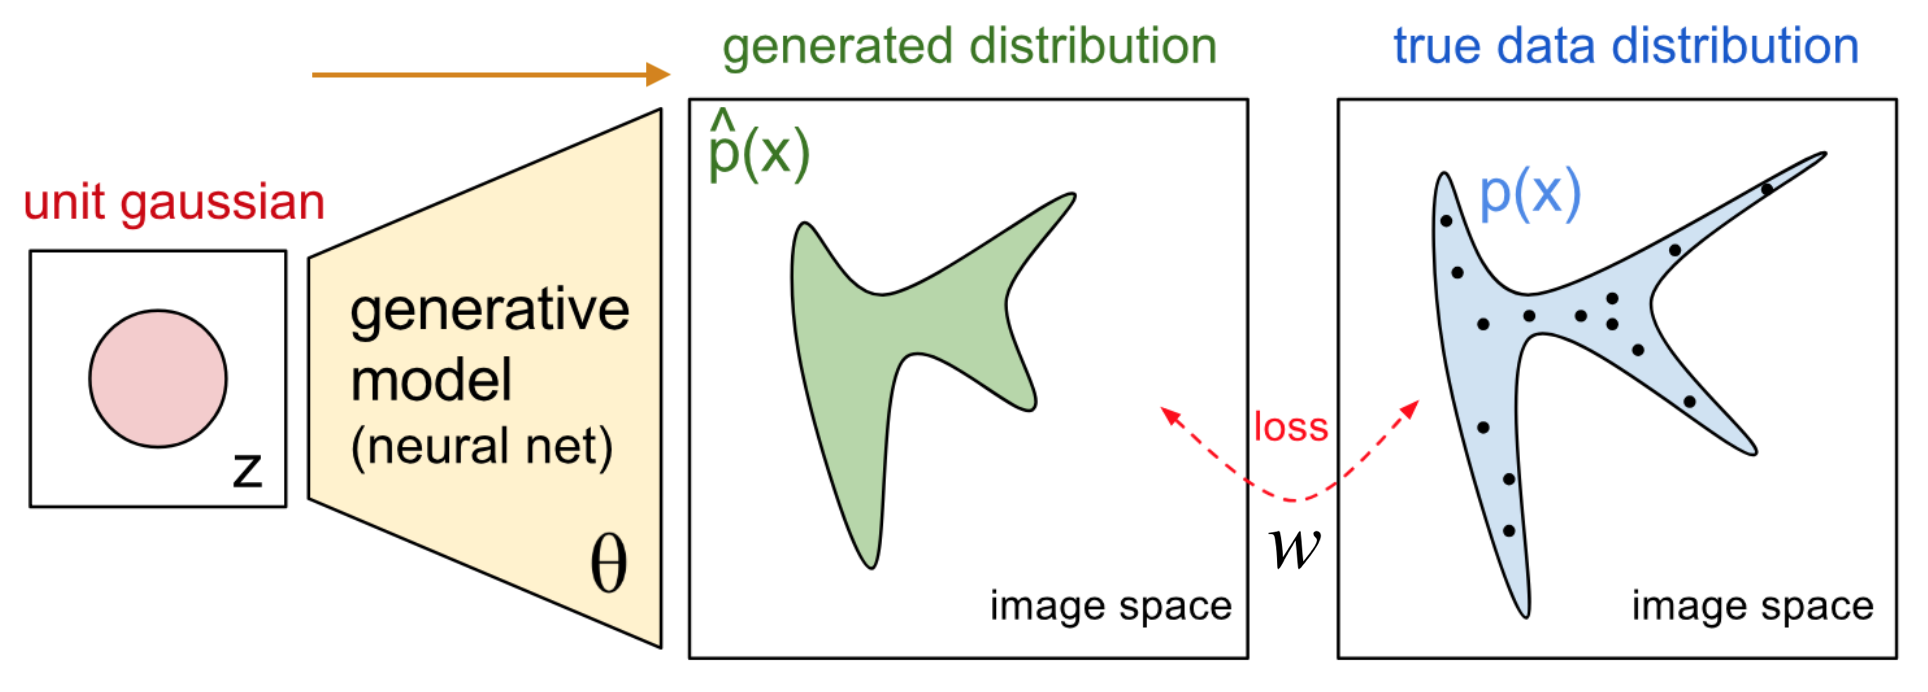
\includegraphics[scale=0.4]{{figures/gen_models_GAN.png}}
\caption{生成对抗网络框架}
\label{fig:GAN_framework}
\end{figure}

\section{生成对抗网络}
与WGAN一样,GAN也是由两张网络构成——$g_{\theta}$和$f_{\Vw}$。GAN中$g_{\theta}$网络的作用依然是把已知分布$\mathcal{Z}$变换为目标分布$p_{r}$,而$f_{\Vw}$网络则与WGAN完全不同。GAN中的$f_{\Vw}$扮演的是“判定者”的角色,它像一个裁判那样判定$g_{\theta}$输出的样本是否来自于训练集背后的真实分布$p_{r}$。因此$f_{\Vw}$接受$g_{\theta}$的输出,并输出一个表示其属于目标分布$p_{r}$的概率。我们把GAN中的$g_{\theta}$网络依然称为Generator,而$f_{\Vw}$网络则称为Discriminator。两张神经网络的优化目标分别为:
\begin{itemize}
	\setlength{\itemsep}{0pt}
    \setlength{\parsep}{0pt}
    \setlength{\parskip}{0pt}
	\item Discriminator的优化目标是
		\begin{eqnarray}
		\max_{\Vw} \SetE_{\Vx\sim p_{r}}\big{[}\log f_{\Vw}(\Vx)\big{]} + \SetE_{\Vz\sim\mathcal{Z}}\big{[}\log(1-f_{\Vw}(g_{\theta}(\Vz)))\big{]}
		\end{eqnarray}
	\item Generator的优化目标是
		\begin{eqnarray}
		\min_{\theta} \SetE_{\Vz\sim\mathcal{Z}}\big{[}\log(1-f_{\Vw}(g_{\theta}(\Vz)))\big{]}
		\end{eqnarray}
\end{itemize}
注意GAN中的$f_{\Vw}$作为Discriminator其输出是$0$到$1$之间的概率值。

GAN的训练过程与WGAN十分类似:
\begin{itemize}
	\setlength{\itemsep}{0pt}
    \setlength{\parsep}{0pt}
    \setlength{\parskip}{0pt}
    \item 固定$\theta$,找到最优的$f_{\Vw}$使得Discriminator的判别准确率最高。
    \item 固定$\Vw$,将$\SetE_{\Vz\sim\mathcal{Z}}\big{[}\log(1-f_{\Vw}(g_{\theta}(\Vz)))\big{]}$作为$g_{\theta}$的loss对$\theta$进行一次梯度下降。
\end{itemize}
重复上面两个步骤直到收敛。GAN的算法框架如下:
\begin{center}
\begin{tabularx}{\textwidth}{X}
\toprule 
\textbf{{GAN}算法框架}\\
\midrule
\textbf{输入}:已知分布$\mathcal{Z}$,梯度下降步长$\alpha$,求$f_{\Vw}$最优解的迭代次数$n_{\rm{discriminator}}$\\
\textbf{初始}:$\Vw$和$\theta$的初始值\\
\textbf{重复}:当$\theta$未收敛时\\
\parbox{1\textwidth}{\begin{enumerate}[topsep=0pt]
    \setlength{\itemsep}{0pt}
    \setlength{\parsep}{0pt}
    \setlength{\parskip}{0pt}
    \item 训练$f_{\Vw}$,在$\Vw$上进行$n_{\rm{discriminator}}$次梯度下降:
    \item $\quad$从训练集中随机采集$m$个样本$\{\Vx^{(i)}\}_{i=1}^{m}$
    \item $\quad$从已知分布$\mathcal{Z}$中随机采集$m$个样本$\{\Vz^{(i)}\}_{i=1}^{m}$
    \item $\quad$计算关于$\Vw$的梯度$G_{\Vw}\gets\nabla_{\Vw}\frac{1}{m}\sum_{i=1}^{m}\big{[} \log f_{\Vw}(\Vx^{(i)})+\log(1-f_{\Vw}(g_{\theta}(\Vz^{(i)}))) \big{]}$
    \item $\quad$更新参数$\Vw=\Vw + \alpha G_{\Vw}$
    \item 训练$g_{\theta}$,在$\theta$上进行一次梯度下降:
    \item $\quad$从已知分布$\mathcal{Z}$中随机采集$m$个样本$\{\Vz^{(i)}\}_{i=1}^{m}$
    \item $\quad$计算关于$\theta$的梯度$G_{\theta}\gets\nabla_{\theta}\frac{1}{m}\sum_{i=1}^{m}\log(1-f_{\Vw}(g_{\theta}(\Vz^{(i)})))$
    \item $\quad$更新参数$\theta=\theta + \alpha G_{\theta}$
\end{enumerate}}\\\bottomrule
\end{tabularx}
\end{center}

在具体的代码实现中,对于同一个$p_{r}$,GAN和WGAN唯一显著的不同是GAN在WGAN的$f_{\Vw}$网络后面添加了一个Logistic层,从而把$f_{\Vw}$的输出限定在了$(0,1)$区间。这一点点不同使得整个模型的意义发生了巨大变化。在本章第一节我们曾经提到过GAN的目标函数是最小化$g_{\theta}(\mathcal{Z})$与$p_{r}$的JS散度。事实上GAN在其训练过程中并没显式地沿着减小JS散度的方向去优化,GAN只是在$\theta$最终收敛时$g_{\theta}(\mathcal{Z})$与$p_{r}$的JS散度达到最小[\cite{goodfellow_14}]。


\section{变分自编码器}
前面两节中我们介绍的WGAN和GAN都是把某个已知分布变换近似为真实分布来得到生成模型(图\ref{fig:GAN_framework})。此外还有一类模型采用的是反向思路——把真实分布变换近似为已知分布来达到学习目标(图\ref{fig:VAE_framework},注意图中左上角的箭头方向)。这类模型的代表是变分自编码器(VAE)。VAE在训练过程中尽量使真实分布变换后的分布与已知分布的KL散度最小。
\begin{figure}[ht]
\centering
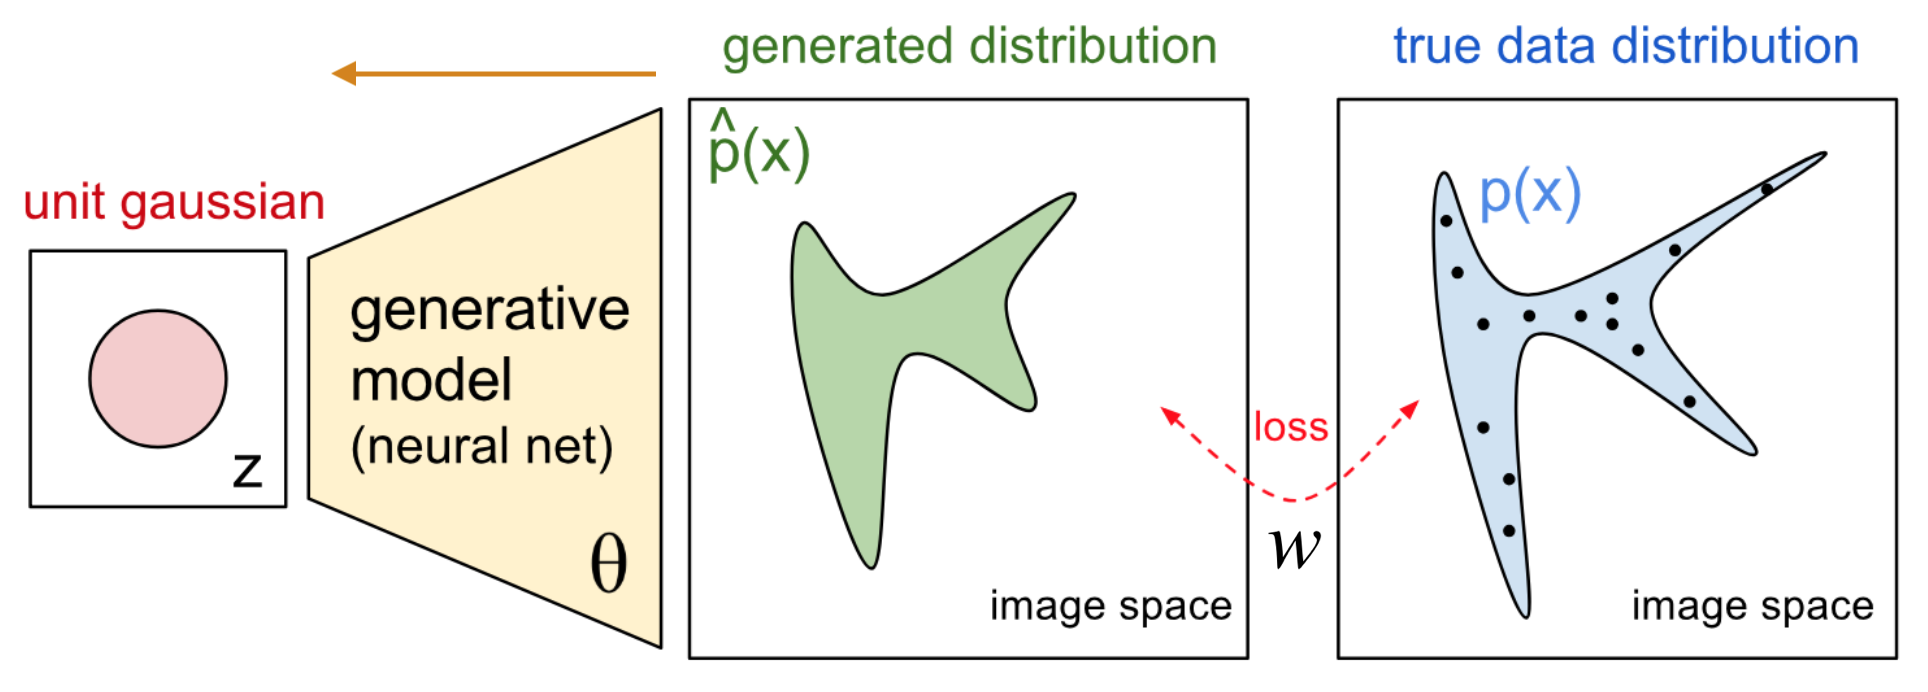
\includegraphics[scale=0.4]{{figures/gen_models_VAE.png}}
\caption{变分自编码器框架}
\label{fig:VAE_framework}
\end{figure}

\subsection{VAE架构}
VAE同样由两张神经网络构成:第一张网络$q_{\theta}(\Vz|\Vx)$称为编码器(Encoder),它把来自于目标分布$p_{r}$(训练集)的样本$\Vx$编码为来自已知分布$\mathcal{Z}$的样本$\Vz$;第二张网络$p_{\Vw}(\Vx|\Vz)$称为解码器(Decoder),它把Encoder编码得到的$\Vz$还原为$\Vx$。解码器的存在有两个意义:
\begin{itemize}
	\setlength{\itemsep}{0pt}
    \setlength{\parsep}{0pt}
    \setlength{\parskip}{0pt}
	\item 辅助编码器对目标分布$p_{r}$向已知分布$\mathcal{Z}$的变换\\
			编码器在变换分布的过程中难免丢失信息,如果信息丢失过多则解码器将很难还原。解码器会根据对原始输入的还原情况评估信息的丢失程度并传递给编码器,从而辅助其改进。
	\item 训练完成后解码器即为目标生成模型(即GAN框架中的Generator)\\
			训练完成之后若需要生成来自于$p_{r}$的样本,只需对已知分布$\mathcal{Z}$采样并输入到解码器中,对应的解码器输出即为来自于$p_{r}$的样本。
\end{itemize}
至此VAE和自编码器(Autoencoder, AE)并无区别,这是因为有一个问题还未解决——编码器如何将目标分布$p_{r}$变换为已知分布$\mathcal{Z}$呢?自编码器的学习目标是最大化解码器的还原程度:
\begin{eqnarray}
\max_{\theta,\Vw}\SetE_{\Vz\sim q_{\theta}(\Vz|\Vx)}\big{[} \log p_{\Vw}(\Vx|\Vz) \big{]}
\end{eqnarray}
既然我们希望的是编码器$q_{\theta}(\Vz|\Vx)$的输出$\Vz$来自于已知分布$\mathcal{Z}$,那么只要$q_{\theta}(\Vz|\Vx)\approx\mathcal{Z}$便可以满足我们的要求,因此我们可以把此作为学习目标的一部分。选择KL散度作为分布相似度的衡量,则VAE的学习目标为
\begin{eqnarray}
\max_{\theta,\Vw}\SetE_{\Vz\sim q_{\theta}(\Vz|\Vx)}\big{[} \log p_{\Vw}(\Vx|\Vz) \big{]} - D_{KL}(q_{\theta}(\Vz|\Vx)\|\mathcal{Z}) \label{eqn:VAE_loss}
\end{eqnarray}
上式(\ref{eqn:VAE_loss})的含义是:解码器对编码器变换之后样本的还原要尽可能的高,且编码器变换之后的样本要尽可能的服从已知分布$\mathcal{Z}$。

可以看出,编码器和解码器两张网络在VAE的架构中相比于对抗,更多的是协作。

我想如果读者是第一次接触VAE,那么你肯定会问:变分自编码器中的“变分”体现在哪里?变分的思想是从概率模型(Probablity Model)的角度体现出来的。这是对VAE的另一种解读。

\subsection{变分与概率图模型}
从概率图模型的角度我们便可以看到VAE中所蕴含的变分思想。概率图模型(图\ref{fig:VAE_graphical_model})认为数据$\Vx$的分布收到其背后的隐变量$\Vz$的影响,即$p(\Vx|\Vz)$,而二者的联合分布为$p(\Vx,\Vz)=p(\Vx|\Vx)p(\Vz)$。
\begin{figure}[ht]
\centering
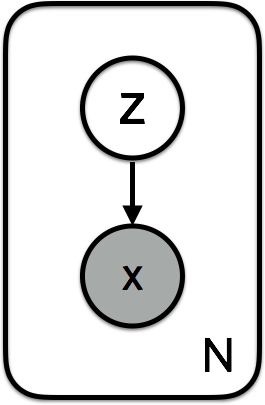
\includegraphics[scale=0.4]{{figures/VAE_graphical_model.png}}
\caption{变分自编码器的概率图模型}
\label{fig:VAE_graphical_model}
\end{figure}
于是$\Vx$的样本生成过程分为两步:
\begin{enumerate}
	\setlength{\itemsep}{0pt}
    \setlength{\parsep}{0pt}
    \setlength{\parskip}{0pt}
	\item 对隐变量采样得到$\Vz_{i}\sim p(\Vz)$
	\item 对数据采样得到$\Vx_{i}\sim p(\Vx|\Vz_{i})$
\end{enumerate}
现在我们要做的事情是对这个概率图模型进行推断,希望根据观测到的样本数据$\Vx$来还原出背后的隐变量分布,即$\Vz$的后验概率$p(\Vz|\Vx)$。根据贝叶斯公式我们有
\begin{eqnarray}
p(\Vz|\Vx) = \frac{p(\Vx|\Vz)p(\Vz)}{p(\Vx)}
\end{eqnarray}
对于上式右边部分的分母$p(\Vx)$有$p(\Vx)=\int_{\Vz}p(\Vx|\Vz)p(\Vz)d\Vz$,代入上式可得
\begin{eqnarray}
p(\Vz|\Vx) = \frac{p(\Vx|\Vz)p(\Vz)}{\int_{\Vz}p(\Vx|\Vz)p(\Vz)d\Vz}
\end{eqnarray}
然而求解$\int_{\Vz}p(\Vx|\Vz)p(\Vz)d\Vz$需要遍历整个$\mathcal{Z}$空间,这在求解实际问题中是不可能的,因此我们需要对后验概率$p(\Vz|\Vx)$进行近似求解。对于这类问题一般有两个方法——马尔可夫链蒙特卡洛法和变分推断法。马尔可夫链蒙特卡洛法精度较高,但由于要生成大量的采样其时间消耗巨大;而变分推断法相对精度不高但求解速度很快。在这里我们选择后者。

变分推断通过一个分布族$q_{\lambda}(\Vz|\Vx)$来近似后验概率$p(\Vz|\Vx)$,其中$\lambda$表征了分布族中的不同分布。最常用的分布族之一就是高斯分布族,此时$\lambda=(\mu,\sigma^{2})$。既然我们要在分布族$q_{\lambda}(\Vz|\Vx)$中找到最接近$p(\Vz|\Vx)$的分布$q_{\lambda}^{*}(\Vz|\Vx)$,这就又遇到了衡量分布相似度的问题,在变分推断中我们选择的是最常见的KL散度。于是原问题现在转化为了一个最优化问题:
\begin{eqnarray}
q_{\lambda}^{*}(\Vz|\Vx) = \mathop{\argmin}_{\lambda}D_{KL}(q_{\lambda}(\Vz|\Vx)\|p(\Vz|\Vx))
\end{eqnarray}
根据KL散度的定义有
\begin{eqnarray}
D_{KL}(q_{\lambda}(\Vz|\Vx)\|p(\Vz|\Vx))
&=& \int_{\Vz}\log\Big{(} \frac{q_{\lambda}(\Vz|\Vx)}{p(\Vz|\Vx)} \Big{)}q_{\lambda}(\Vz|\Vx)d\Vz \nonumber\\
&=& \int_{\Vz}\log\Big{(} \frac{q_{\lambda}(\Vz|\Vx)}{p(\Vx,\Vz)}p(\Vx) \Big{)}q_{\lambda}(\Vz|\Vx)d\Vz \nonumber\\
&=& \int_{\Vz}\log\Big{(} q_{\lambda}(\Vz|\Vx) - p(\Vx,\Vz) + p(\Vx) \Big{)}q_{\lambda}(\Vz|\Vx)d\Vz \nonumber\\
&=& \SetE_{\Vz\sim q}[\log q_{\lambda}(\Vz|\Vx)] - \SetE_{\Vz\sim q}[\log p(\Vx,\Vz)] + \int_{\Vz}\log p(\Vx)q_{\lambda}(\Vz|\Vx)d\Vz \nonumber\\
&=& \SetE_{\Vz\sim q}[\log q_{\lambda}(\Vz|\Vx)] - \SetE_{\Vz\sim q}[\log p(\Vx,\Vz)] + \log p(\Vx) \label{eqn:ELBO_1}
\end{eqnarray}
上式(\ref{eqn:ELBO_1})经过简单变换后得到
\begin{eqnarray}
\log p(\Vx) = \underbrace{\SetE_{\Vz\sim q}[\log p(\Vx,\Vz)] - \SetE_{\Vz\sim q}[\log q_{\lambda}(\Vz|\Vx)]}_{\rm{ELBO}(\lambda)} + D_{KL}(q_{\lambda}(\Vz|\Vx)\|p(\Vz|\Vx)) \label{eqn:ELBO_2}
\end{eqnarray}
注意式(\ref{eqn:ELBO_2})中的$\log p(\Vx)$的值是固定不变的,且KL散度恒大于等于$0$,因此最小化$D_{KL}(q_{\lambda}(\Vz|\Vx)\|p(\Vz|\Vx))$等价于最大化$\SetE_{\Vz\sim q}[\log p(\Vx,\Vz)] - \SetE_{\Vz\sim q}[\log q_{\lambda}(\Vz|\Vx)]$。$\SetE_{\Vz\sim q}[\log p(\Vx,\Vz)] - \SetE_{\Vz\sim q}[\log q_{\lambda}(\Vz|\Vx)]$称为“证据下界”(Evidence Lower BOund, ELBO)。

接下来我们再对$\rm{ELBO}(\lambda)$进行一系列简单的变换(这是为了接下来与VAE产生联系):
\begin{eqnarray}
\rm{ELBO}(\lambda)
&=& \SetE_{\Vz\sim q}[\log p(\Vx,\Vz)] - \SetE_{\Vz\sim q}[\log q_{\lambda}(\Vz|\Vx)] \nonumber\\
&=& \SetE_{\Vz\sim q}[\log p(\Vx|\Vz)p(\Vz)] - \SetE_{\Vz\sim q}[\log q_{\lambda}(\Vz|\Vx)] \nonumber\\
&=& \SetE_{\Vz\sim q}[\log p(\Vx|\Vz)] + \SetE_{\Vz\sim q}[\log p(\Vz)] - \SetE_{\Vz\sim q}[\log q_{\lambda}(\Vz|\Vx)] \nonumber\\
&=& \SetE_{\Vz\sim q}[\log p(\Vx|\Vz)] - \SetE_{\Vz\sim q}\Big{[}\log \frac{q_{\lambda}(\Vz|\Vx)}{p(\Vz)}\Big{]} \nonumber\\
&=& \SetE_{\Vz\sim q}[\log p(\Vx|\Vz)] - D_{KL}(q_{\lambda}(\Vz|\Vx)\|p(\Vz))
\end{eqnarray}

现在我们把上面在概率图模型上的数学推导与VAE联系起来。首先我们用一张参数为$\theta$神经网络作为$q_{\theta}(\Vz|\Vx)$,该网络扮演着近似推断后验概率$p(\Vz|\Vx)$的角色,所以称为“推断网络”;然后我们用另一张参数为$\Vw$的神经网络作为$p_{\Vw}(\Vx|\Vz)$,该网络用于给定隐变量$\Vz$之后生成$\Vx$,所以称为“生成网络”。推断网络接受的输入为数据样本$\Vx$,输出隐变量$\Vz$;生成网络的输入为隐变量$\Vz$,输出为生成的$\Vx$。于是两张网络通过隐变量$\Vz$连接在一起,推断网络在前生成网络在后。组合网络的参数为$\{\theta,\Vw\}$,其训练的目标函数为:
\begin{eqnarray}
\max_{\theta,\Vw}\rm{ELBO}(\theta,\Vw) &=& \max_{\theta,\Vw}\SetE_{\Vz\sim q_{\theta}(\Vz|\Vx)}[\log p_{\Vw}(\Vx|\Vz)] - D_{KL}(q_{\theta}(\Vz|\Vx)\|\mathcal{Z}) \label{eqn:VAE_ELBO_objective}
\end{eqnarray}
组合网络的目标函数式(\ref{eqn:VAE_ELBO_objective})与上一节中VAE的目标函数式(\ref{eqn:VAE_loss})完全一致。而这里的推断网络和生成网络分别是VAE中的编码器和解码器。从概率图模型的角度,VAE的训练过程事实上是在最大化变分推断中的ELBO。这就是变分自编码器中变分的来源。


\section{受限玻尔兹曼机}
前面几个章节中介绍的生成模型都是通过变换函数间接学习样本数据真实分布,本节中我们将会介绍一些通过最大似然估计直接学习样本数据真实分布的生成模型,其中受限玻尔兹曼机是这类生成模型的代表。在介绍受限玻尔兹曼机之前,我们需要先了解另外两个模型——霍普菲尔德网络(Hopfield Network, HN)和玻尔兹曼机。

\subsection{霍普菲尔德网络}
霍普菲尔德网络是一个全连接网络。所谓全连接指的是网络中的每一个神经元都和其他所有神经元连接在一起(图\ref{fig:hopfield_network})。霍普菲尔德网络最大的意义在于它在神经网络中引入了\textbf{能量}的概念。后来所有基于能量(Energy-based)的神经网络都可以追溯到霍普菲尔德网络。
\begin{figure}[ht]
\centering
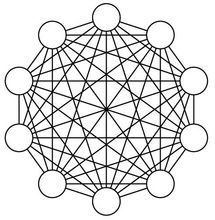
\includegraphics[scale=0.9]{{figures/hopfield_network.jpg}}
\caption{霍普菲尔德网络}
\label{fig:hopfield_network}
\end{figure}

\subsubsection{霍普菲尔德网络的定义}
一个霍普菲尔德网络由$N$个神经元构成,每个神经元的激发函数是符号函数,于是每个神经元有两个状态——激发态和静息态,两种状态在数学上的值分别定义为$1$和$-1$;接下来再定义神经元$j$到神经元$i$的连接权重为$\MW_{ij}$,则所有的参数$\MW_{ij}$构成了连接矩阵$\MW$。霍普菲尔德网络中的连接$\MW_{ij}$有两个约束条件:
\begin{itemize}
	\setlength{\itemsep}{0pt}
    \setlength{\parsep}{0pt}
    \setlength{\parskip}{0pt}
	\item 对称性: $\MW_{ij}$ = $\MW_{ji}$
	\item 不存在自连接: $\MW_{ii} = 0$
\end{itemize}
设神经元$i$的状态为$x_{i}$则
\begin{eqnarray}
x_{i} =
\begin{cases}
1   & \quad  \sum_{j}^{} \MW_{ij}x_{j} \geq 0\\
-1  & \quad  \sum_{j}^{} \MW_{ij}x_{j} < 0 
\end{cases} \nonumber
\end{eqnarray}
即
\begin{eqnarray}
x_{i} = \mathop{\rm sgn}(\sum_{j}^{} \MW_{ij}x_{j}) \nonumber
\end{eqnarray}

可以看出,假如给霍普菲尔德网络一个初始状态,网络将会不断的自我演化更新直至稳态或震荡。网络状态的更新有两种方式:
\begin{itemize}
	\setlength{\itemsep}{0pt}
    \setlength{\parsep}{0pt}
    \setlength{\parskip}{0pt}
    \item 同步更新:所有的神经元同时计算在当前时刻所接收到的输入,之后在同一时刻一齐更新到新的状态。
	\item 异步更新:按照依次或随机选择一个神经元,根据其接收的输入更新其状态。
\end{itemize}
当满足连接权重的对称性和不存在自连接两个约束条件时,使用异步更新的方式更新网络状态,可以保证霍普菲尔德网络收敛(霍普菲尔德网络并非本书讨论的重点内容,因此在本章节将不再深入的讨论其收敛性证明)。下面我们要引入\textbf{能量}的概念。

\subsubsection{回声网络与能量}
我们通过一种更加简单的模型——双向关联记忆网络(Bidirectional Associative Memory, BAM)来引入能量。BAM又称为回声网络(Resonance Network),如图\ref{fig:bam},其基本组成单元与霍普菲尔德网络的神经元一样,激发函数为符号函数。回声网络可以看作是一个两层网络,两层之间全连接,层内无连接,也不存在自连接。
\begin{figure}[ht]
\centering
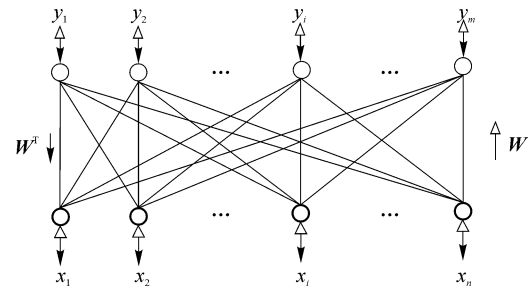
\includegraphics[scale=0.8]{{figures/bam.png}}
\caption{回声网络}
\label{fig:bam}
\end{figure}

图\ref{fig:bam}中所示的回声网络由两层构成,分别记为$x$层和$y$层。设其输入为$n$维行向量$\Vx$,输出为$k$维行向量$\Vy$,两层之间$n \times k$的权重矩阵为$\MW$,网络第一次更新时更新$y$层得到$\Vy_{(0)}$,则有
\begin{eqnarray}
y_{(0)} = \mathop{\rm sgn}(\Vx_{(0)}\MW) \nonumber
\end{eqnarray}
接着以$\Vy_{(0)}$作为输入,向左传更新$x$层,得到$\Vx_{(0)}$
\begin{eqnarray}
\Vx_{(1)}^\top = \mathop{\rm sgn}(\MW\Vy_{(0)}^\top)\nonumber
\end{eqnarray}
再以$\Vx_{(1)}$作为输入,向右传更新$y$层,得到$\Vy_{(1)}$
\begin{eqnarray}
\Vy_{(1)} = \mathop{\rm sgn}(\Vx_{1}\MW)\nonumber
\end{eqnarray}
归纳可得:
\begin{eqnarray}
\Vy_{(i)} &=& \mathop{\rm sgn}(\Vx_{(i)}\MW)\nonumber\\
\Vx_{(i)}^\top &=& \mathop{\rm sgn}(\MW\Vy_{(i)}^\top)\nonumber
\end{eqnarray}
如果BAM最终达到了稳定状态,即向量$\Vx$和$\Vy$都不再发生变化,记此时的$\Vx$,$\Vy$分别为$\Vx_{(m)} \Vy_{(m)}$,则有
\begin{eqnarray}
\Vy_{(m)} = \mathop{\rm sgn}(\Vx_{(m)}\MW) \quad \quad \Vx_{(m)}^\top = \mathop{\rm sgn}(\MW\Vy_{(m)}^\top)\nonumber
\end{eqnarray}
下面我们开始逐步引入能量。首先,定义一个关于$\Vx_{i}$的“激发向量”(excitation vector)$\Ve$,那么对于任意一对向量$(\Vx_{(i)},\Vy_{(i)})$有:
\begin{eqnarray}
\Ve^\top = \MW\Vy_{(i)}^\top\nonumber
\end{eqnarray}

如果$(\Vx,\Vy)$是最终的稳定向量对,则满足
\begin{eqnarray}
\mathop{\rm sgn}(\Ve) = \Vx\nonumber
\end{eqnarray}
直观上,如果向量$\Ve$想要满足这个条件,那么它每一项的符号都需要与$\Vx$相同,意味着$\Ve$足够靠近$\Vx$。可以想象一下,在二维空间,$\Ve$和$\Vx$落在同一个象限,在三维空间,$\Ve$和$\Vx$落在同一个卦限,以此类推,维数越高则对$\Ve$的约束越强。根据内积的定义,对于同样长度的$\Ve$,越靠近$\Vx_{0}$,两者的内积越大,因此是否可以使用$\Vx$和$\Ve$的内积来作为一个衡量回声网络收敛到稳态的指数呢?内积
\begin{eqnarray}
\langle\Vx,\Ve\rangle 
&=& \Vx\Ve^\top\nonumber\\
&=& \Vx\MW\Vy^\top\nonumber\\
&=& \Vx(\sum_{j=1}^{k}\MW_{1j}\Vy_{j},\sum_{j=1}^{k}\MW_{2j}\Vy_{j},\cdots,\sum_{j=1}^{k}\MW_{nj}\Vy_{j})\nonumber\\
&=& (\Vx_{1},\Vx_{2},...,\Vx_{n})(\sum_{j=1}^{k}\MW_{1j}\Vy_{j},\sum_{j=1}^{k}\MW_{2j}\Vy_{j},\cdots,\sum_{j=1}^{k}\MW_{nj}\Vy_{j})\nonumber\\
&=& \sum_{i=1}^{n}\Vx_{i}\sum_{j=1}^{k}\MW_{ij}\Vy_{j}\nonumber
\end{eqnarray}
$\Vx_{i}$和$\Vy_{j}$的取值只有$\pm1$,在回声网络处于稳态时,对于每一个$\Vx_{i}\sum_{j=1}^{k}\MW_{ij}\Vy_{j}$,$\Vx_{i}$与$\sum_{j=1}^{k}\MW_{ij}\Vy_{j}$的符号相同,则有每一个$\Vx_{i}\sum_{j=1}^{k}\MW_{ij}\Vy_{j}\geq0$,固定$\MW$和$\Vy_{0}$改变$\Vx_{0}$中某一项$\Vx_{s}$的符号(记为$\Vx_{s}^{'}$),则对应的$\Vx_{s}^{'}\sum_{j=1}^{k}\MW_{sj}\Vy_{j}\leq0$,于是有
\begin{eqnarray}
\sum_{i=1}^{n}\Vx_{i}\sum_{j=1}^{k}\MW_{ij}\Vy_{j} \geq \sum_{i=1,i\neq s}^{n}\Vx_{i}\sum_{j=1}^{k}\MW_{ij}\Vy_{j} + \Vx_{s}^{'}\sum_{j=1}^{k}\MW_{sj}\Vy_{j}\nonumber
\end{eqnarray}
由此可知,回声网络处于稳态时,$\Vx_{0}$和$\Ve$的内积最大。对于一般的物理系统,能量越低越稳定,因此使用内积的相反数作为能量的定义。于是对回声网络定义能量函数(Energy Function)。给定$\MW$,回声网络在某一时刻的$x$层输出$\Vx$和$y$层的输出$\Vy$,此时回声网络的能量函数定义为:
\begin{eqnarray}
E(\Vx,\Vy) = -\frac{1}{2}\Vx\MW\Vy^\top
\end{eqnarray}
所以对于一个回声网络,稳定态是它能量最小的状态($\frac{1}{2}$项与其他公式中的$\frac{1}{2}$一样是为了方便计算)。

现在我们把回声网络的能量函数推广到更一般的情况。若神经元的激发函数是一个阶跃函数,此时只需对能量函数进行一点点扩展即可。位于左边的$n$维向量$\Vx$和位于右边的$k$维向量$\Vy$分别各增加一维得到$(\Vx_{1},\cdots,\Vx_{n},1)$和 $(\Vy_{1},\cdots,\Vy_{n},1)$。连接权重矩阵$\MW$增加一行一列,与$\Vx$相关的阶跃函数阈值$\theta_{l}$对应写在$\MW$的第$k+1$列上,与$\Vy$相关的阶跃函数阈值${\theta_{r}}$对应写在$\MW$的第$n+1$行,$\MW$对角线上的元素依然保持为$0$。扩展后的能量函数为:
\begin{eqnarray}
E(\Vx,\Vy) = -\frac{1}{2}\Vx\MW\Vy^\top + \frac{1}{2}\theta_{r}\Vy^\top + \frac{1}{2}\Vx\theta_{l}^\top
\end{eqnarray}
下面直接根据回声网络的能量函数推出霍普菲尔德网络的能量函数。

\subsubsection{霍普菲尔德网络的能量函数}
霍普菲尔德网络与回声网络不同,它是一个全连接的网络,没有x层和y层之分。但我们可以利用霍普菲尔德网络的结构特点来把它看作是一个回声网络来处理:
\begin{enumerate}
	\setlength{\itemsep}{0pt}
    \setlength{\parsep}{0pt}
    \setlength{\parskip}{0pt}
	\item 霍普菲尔德网络只有一个$x$层。
	\item 在一个时刻内使用同步更新的方式更新网络。
	\item 假设在$t$时刻之内,$x$层中的所有神经元逐一完成了更新,那么它们($\Vx_{(t)}$)将在下一个时刻作为输入层传递给$t+1$时刻的自己($\Vx_{t+1}$);而它们($\Vx_{t}$)的输入可以看作来自$t-1$时刻的自己($\Vx_{t-1}$)。
	\item 把$\Vx_{t}$层看作回声网络中的$x$层,把$\Vx_{t+1}$层看作回声网络中的$y$层,那么在$t$到$t+1$时刻,完成了一次从$x$层到$y$层的传递更新。
	\item 更进一步,$t$为奇数时$x_{t}$作为x层,$t$为偶数时$x_{t}$作为y层,于是同步更新的Hopfield Network就转化成了一个回声网络。
\end{enumerate}
我们在本书第二章求解循环神经网络的时候已经用到过这种把网络在时间上展开的方法。现在可以直接使用回声网络的能量函数来描述霍普菲尔德网络。因为此时的$y$层就是$x$层自己,所以$\Vx$的阈值${\theta}={\theta_{l}}={\theta_{r}}$。那么霍普菲尔德网络的能量函数为:
\begin{eqnarray}
E(\Vx) 
&=& -\frac{1}{2}\Vx\MW{x}^\top + \frac{1}{2}{\theta}\Vx^\top + \frac{1}{2}\Vx{\theta}^\top\nonumber\\
&=& -\frac{1}{2}\Vx\MW{x}^\top + {\theta}\Vx^\top
\end{eqnarray}
把上式中的矩阵和向量展开,霍普菲尔德网络的能量函数还可以表示成:
\begin{eqnarray}
E(\Vx) = -\frac{1}{2}\sum_{j=1}^{n}\sum_{i=1}^{n}\MW_{ij}\Vx_{i}\Vx_{j} + \sum_{i=1}^{n}\theta_{i}\Vx_{i}
\end{eqnarray}
可以看出霍普菲尔德网络的能量函数是一个二次型,所以往往会有局部最优解。如何避免网络在收敛的过程中陷入局部最优呢?一个很直观的想法是引入概率,从而给网络一定的机会跳出局部最优。把概率引入霍普菲尔德网络并增加一些新的“组件”之后,我们将得到玻尔兹曼机。

\subsection{玻尔兹曼机}
\subsubsection{概率}
我们已经看到,当到霍普菲尔德网络达一个局部最优之后,网络的状态更新便停止了。如果这个局部最优不是全局最优(很可能不是),那么网络永远不能收敛到全局最优。自然而然地我们想到使用概率来给网络一个继续“探寻”下去的机会。如果每个单元(在玻尔兹曼机中通常把神经元称为单元)在确定自己的状态时并非完全取决于它所接收到的输入,而是根据接收的输入以一定的概率来随机产生某个状态,便可以达到这个目的。那么如何去做呢?下面我们要借助一套物理学上的工具来实现我们的目标。

物理学中有一个描述气体分子系统的工具叫玻尔兹曼分布(Boltzmann Distribution)。玻尔兹曼分布首次把统计学引入了物理学中,使用概率把宏观的系统能量和微观的分子状态联系在了一起,并找到了概率和能量的关系。在霍普菲尔德网络中我们已经有了能量,再利用玻尔兹曼分布中能量和概率的关系,便可以把概率引入神经网络。

假设网络中某单个单元$x_{k}$可能的状态有$0$(静息态)和$1$(激发态)两种(注意此时静息态的值为$0$,不是$-1$,这只是为了计算方便,就像在逻辑回归中我们常用$1$和$0$来标记正负样本,而在支持向量机中常用$1$和$-1$来标记正负样本),当$x_{k}$的状态从0($x_{k}=0$)变到1($x_{k}'=1$)时,整个网络能量的变化量为$\Delta E_{i}$。根据上一节我们推出的霍普菲尔德网络能量函数可知
\begin{eqnarray}
\Delta E_{k} 
&=& E(\Vx) - E(\Vx') \nonumber\\
&=& -(\Vx_{k} - \Vx_{k}')(\sum_{i=1}^{n}\MW_{ki} - \theta_{k}) \nonumber\\
&=& \sum_{i=1}^{n}\MW_{ki} - \theta_{k}
\end{eqnarray}
根据玻尔兹曼分布的性质——系统某个状态的能量与该状态出现概率的自然对数的相反数成正比,即$E=-T\log(p)$,有
\begin{eqnarray}
\Delta E_{k} 
&=& E_{\Vx_{k}=0} - E_{\Vx_{k}=1} \nonumber\\
&=& -T\log (p_{\Vx_{k}=0}) - (-T\log (p_{\Vx_{k}=1}))\nonumber
\end{eqnarray}
因为$p_{\Vx_{k}=0}+p_{\Vx_{k}=1}$则
\begin{eqnarray}
\Delta E_{k} = -T\log (1-p_{\Vx_{k}=1}) - (-T\log (p_{\Vx_{k}=1}))\nonumber \\
\frac{\Delta E_{k}}{T} = \log (p_{\Vx_{k}=1}) - \log (1-p_{\Vx_{k}=1})\nonumber \\
\frac{\Delta E_{k}}{T} = \log (\frac{p_{\Vx_{k}=1}}{1-p_{\Vx_{k}=1}})\nonumber \\
-\frac{\Delta E_{k}}{T} = \log (\frac{1-p_{\Vx_{k}=1}}{p_{\Vx_{k}=1}})\nonumber \\
-\frac{\Delta E_{k}}{T} = \log (\frac{1}{p_{\Vx_{k}=1}}-1)\nonumber \\
\exp(-\frac{\Delta E_{k}}{T}) = \frac{1}{p_{\Vx_{k}=1}}-1\nonumber \\
\end{eqnarray}
最终得到神经元$x_{k}$处于激发态($x_{k}=1$)的概率
\begin{eqnarray}
p_{\Vx_{k}=1} = \frac{1}{1+\exp (-\frac{\Delta E_{k}}{T})}
\end{eqnarray}
上式中的比例系数$T$可以看作是网络的“温度”。需要特别注意的是,只有当网络收敛到稳定状态时单元所处的状态才会服从玻尔兹曼分布,对应于物理系统的热平衡(Thermal Equilibrium)。

\subsubsection{概率的意义和隐藏单元}
到目前为止,引入概率之后的网络(姑且称为“随机化的霍普菲尔德网络”)已经有能力跳出局部最优。只要时间足够长,网络将会遍历所有可能的状态。如果把单元看作气体分子,那么整个网络则是一个服从玻尔兹曼分布的系统。而服从某种分布的网络可以用来模拟现实世界的某种服从概率分布/统计的行为。什么意思呢?想象一下,我们对现实世界中的某一个事物进行观察,并使用一组变量来表示观察结果。最终收集到的一系列结果会服从某种分布。然后我们希望使用神经网络来模拟我们的观测结果。这就相当于使用神经网络构建一个网络内部的模型,该模型所服从的分布与观察结果所服从的分布接近甚至相同。如果能够建立这样一个网络,将会非常有用。例如可以通过网络来得到更多的结果而不必进行更多的观测;或者对网络本身进行研究,从而得到对现实世界中该事物产生这样一组观测结果的过程更加深入的认识。

但是,“随机化的霍普菲尔德网络”对于绝大多数的情况完全不能够胜任。这是因为网络本身的结构——“随机化的H霍普菲尔德网络”的单元数目与“描述观测结果的变量”数目相等——造成的。根据玻尔兹曼分布,网络处于热平衡态时,某种状态的出现概率只取决于于它的能量:
\begin{eqnarray}
P_{\alpha} = \frac{\exp(-E_{\alpha})}{\sum_{\beta}\exp(-E_{\beta})}\nonumber
\end{eqnarray}
其中$P_{\alpha}$是处于平衡态时网络状态为$\alpha$的概率,分母是所有可能的状态求和(分母除以比例系数$T$之后是概率,再求和其实就是1)。网络的行为特性由它的连接权重$\MW_{ij}$决定。连接权重$w_{ij}$的变化对网络进入某种状态的概率的影响可以通过该状态的概率对连接权重求偏导得到:
\begin{eqnarray}
\frac{\partial\log P_{\alpha}}{\partial \MW_{ij}} = \frac{1}{T}(\Vx_{i}^{\alpha}\Vx_{j}^{\alpha}-\sum_{\beta}P_{\beta}\Vx_{i}^{\beta}\Vx_{j}^{\beta}) \nonumber
\end{eqnarray}
其中$\Vx_{k}^{\gamma}$表示第$k$个单元$\Vx_{k}$在网络处于状态$\gamma$时的状态(推导过程可以参见玻尔兹曼机的求解过程)。由该式可见,连接权重只通过单元对$(\Vx_{i}\Vx_{j})$影响网络进入某种状态的概率。这意味着“随机化的霍普菲尔德网络”只能捕捉到现实世界中二阶及以下的结构,对更高阶的结构无能为力。例如在一个三单元网络看来,一组状态$((0,0,0),(0,1,1),(1,0,1),(1,1,0))$与另一组状态$((1,1,1),(1,0,0),(0,1,0),(0,0,1))$是一样的,因为他们的均值与内部相关性是相等的。如何解决这个问题?一个直观的想法就是引入更多的单元去捕捉那些高阶的结构。这些后来引入的单元并不用来表示现实世界的某个观测变量,它们被称为隐藏单元(Hidden Units);而原本的那些对应于观测结果的单元被称为可见单元(Visible Units)。这种“加入隐藏单元的随机化霍普菲尔德网络”就是玻尔兹曼机(图\ref{fig:bm})。
\begin{figure}[ht]
\centering
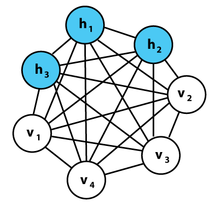
\includegraphics[scale=0.8]{{figures/bm.png}}
\caption{玻尔兹曼机}
\label{fig:bm}
\end{figure}

玻尔兹曼机中的可见单元可以看作是网络中与现实世界的接口,而现实世界中得到的观测结果变量同样可以看作是现实世界中与网络的接口。网络内部的模型建立的越好,两个接口越接近。所谓的“两个接口接近”事实上指的是:现实世界中的观测结果变量所服从的真实分布,与网络中的可见单元所服从的分布相似。我们再一次遇到了衡量两个分布相似度的问题。在玻尔兹曼机中,我们使用KL距离,这其实意味着玻尔兹曼机是在\textbf{通过最大似然估计直接学习样本数据真实分布}。

把可见单元记为$\Vv$,隐藏单元记作$\Vh$,则$|\Vv|$个可见单元可能的状态共有$2^{|\Vv|}$个,相应地,观测结果变量可能的状态也有$2^{|\Vv|}$个。
% 把观测结果变量进入第$\alpha$个状态的概率记为$P_{r}(\Vv_{\alpha})$,可见单元进入同一个状态的概率记为$P_{\Vw}(\Vv_{\alpha})$。
观测结果的$P_{r}(\Vv)$是目标分布,我们希望网络的$P_{\Vw}(\Vv)$尽可能地靠近前者。二者的KL距离为
\begin{eqnarray}
D_{KL}(P_{r}(\Vv)\|P_{\Vw}(\Vv)) = \sum_{\Vv}P_{r}(\Vv)\log\frac{P_{r}(\Vv)}{P_{\Vw}(\Vv)}
\end{eqnarray}
观测结果的分布$P_{r}(\Vv)$是已知的。可见单元的分布$P_{\Vw}(\Vv)$由该状态对应的能量$E_{\Vv,\Vh}$决定,而$E_{\Vv,\Vh}$唯一由网络的连接权重$\Vw_{ij}$确定。所以二者的KL距离是关于连接权重$\Vw_{ij}$的函数,于是便可以采用梯度下降法来训练网络。由于篇幅所限,本书就不再继续推导下去了,感兴趣的读者可以阅读相应的文献,在这里我们直接给出结果:
\begin{eqnarray}
\frac{\partial D_{KL}}{\partial \Vw_{ij}} = -\frac{1}{T}(p_{ij} - p'_{ij})
\end{eqnarray}
其中$p_{ij}$是网络到达平衡态后固定可见单元时$(x_{i},x_{j})$同时被激发的概率;$p'_{ij}$是网络到达平衡态时$(x_{i},x_{j})$同时被激发的概率;单元$x_{i}$为某一个可见单元或隐藏单元。

可以看出在训练玻尔兹曼机时,每次调整完连接权重$\Vw_{ij}$都要等待网络进入平衡态后,分别统计$p_{ij}$和$p'_{ij}$,才能进行一次梯度下降更新,训练效率极其低下。当网络的规模变大、结构越发复杂的时候,网络进入平衡态需要很长时间,所以玻尔兹曼机在实际使用中的效果并不理想。若想使得玻尔兹曼机能够用于实践,就不得不对其网络复杂度进行控制。网络复杂度是由单元和单元间的连接决定的,在保持单元数目不变的前提下,那就只能对单元间连接的数目进行限制了——受限玻尔兹曼机。

\subsection{受限玻尔兹曼机}
去掉玻尔兹曼机中可见单元之间的连接,再去掉隐藏单元之间的连接,就得到了受限玻尔兹曼机。受限玻尔兹曼机是一个双层无向网络,结构与我们在回声网络很相似(图\ref{fig:rbm})。通常受限玻尔兹曼机中单元的激发函数是sigmoid函。
\begin{figure}[ht]
\centering
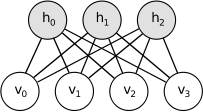
\includegraphics[scale=0.9]{{figures/rbm.png}}
\caption{受限玻尔兹曼机}
\label{fig:rbm}
\end{figure}

受限玻尔兹曼机中能量的定义与玻尔兹曼机保持一致。设网络由$m$个可见单元和$n$个隐藏单元构成,则受限玻尔兹曼机的能量定义为
\begin{eqnarray}
E(\Vv,\Vh) = -\sum_{i=1}^{n}\sum_{j=1}^{m}\Vw_{ij}\Vh_{i}\Vv_{j} - \sum_{j=1}^{m}\Vb_{j}\Vv_{j} - \sum_{i=1}^{n}\Vc_{i}\Vh_{i}
\end{eqnarray}
其中$\Vw_{ij}$是可见单元$\Vv_{j}$与隐藏单元$\Vh_{i}$之间的连接权重,$\Vb_{j}$和$\Vc_{i}$分别是可见单元$\Vv_{j}$与隐藏单元$\Vh_{i}$的偏置。注意,当该项定义为“阈值”的时候,它大于$0$,而当该项定义为“偏置”的时候,它小于$0$。因此受限玻尔兹曼机中能量函数的“偏置项”与玻尔兹曼机中的“阈值项”的符号不同,但意义是一样的。

受限玻尔兹曼机的求解比玻尔兹曼机高效很多,常用的有Gibbs采样、变分法、对比分歧算法(Constrastive Divergence)等等。受限玻尔兹曼机这样一个“浅网络”表达能力不够强,随着深度学习的崛起,受限玻尔兹曼机已经用的比较少了。
\newpage
\section*{参考文献}\printbibliography[segment=\therefsegment,heading=none]

\newpage
\part{PartII}

% !Mode:: "TeX:UTF-8"
% !TEX root = ../Cuckoo.tex

\clearpage

%\setcounter{chapter}{1}\setcounter{page}{1}
\fancyhead[EC]{\small\small\thepage\rm\hfill \small 书名 \hfill}
\fancyhead[OC]{\rm\hfill\small 第4章\quad 第4章标题 \hfill\thepage}

\chapter{第4章}





\section{小结}




\section*{参考文献}\printbibliography[segment=\therefsegment,heading=none]

% !Mode:: "TeX:UTF-8"
% !TEX root = ../Book.tex

\clearpage

%\setcounter{chapter}{5}\setcounter{page}{1}
\fancyhead[EC]{\small\small\thepage\rm\hfill \small 书名 \hfill}
\fancyhead[OC]{\rm\hfill\small 第5章\quad 第5章标题 \hfill\thepage}




\chapter{第5章}



\section{小结}


\section*{参考文献}\printbibliography[segment=\therefsegment,heading=none]

% !Mode:: "TeX:UTF-8"
% !TEX root = ../Book.tex

\clearpage

%\setcounter{chapter}{6}\setcounter{page}{1}
\fancyhead[EC]{\small\small\thepage\rm\hfill \small 书名 \hfill}
\fancyhead[OC]{\rm\hfill\small 第6章\quad 第6章标题 \hfill\thepage}

\chapter{第6章}



\section{小结}



\section*{参考文献}\printbibliography[segment=\therefsegment,heading=none]

% !Mode:: "TeX:UTF-8"
% !TEX root = ../Book.tex

\clearpage

%\setcounter{chapter}{7}\setcounter{page}{1}
\fancyhead[EC]{\small\small\thepage\rm\hfill \small 书名 \hfill}
\fancyhead[OC]{\rm\hfill\small 第7章\quad 第7章标题 \hfill\thepage}

\chapter{第7章}




\section{小结}



\section*{参考文献}\printbibliography[segment=\therefsegment,heading=none]

% !Mode:: "TeX:UTF-8"
% !TEX root = ../Book.tex

\clearpage

%\setcounter{chapter}{9}\setcounter{page}{1}
\fancyhead[EC]{\small\small\thepage\rm\hfill \small 书名 \hfill}
\fancyhead[OC]{\rm\hfill\small 第8章\quad 第8章标题 \hfill\thepage}

\chapter{第8章}



\section{小结}



\section*{参考文献}\printbibliography[segment=\therefsegment,heading=none]

\newpage
\part{PartIII}

% !Mode:: "TeX:UTF-8"
% !TEX root = ../Book.tex

\clearpage

%\setcounter{chapter}{12}\setcounter{page}{1}
\fancyhead[EC]{\small\small\thepage\rm\hfill \small 书名 \hfill}
\fancyhead[OC]{\rm\hfill\small 第9章\quad 第9章标题 \hfill\thepage}

\chapter{第9章}
\section{第1节}



\section{小结}


\section*{参考文献}\printbibliography[segment=\therefsegment,heading=none]

% !Mode:: "TeX:UTF-8"
% !TEX root = ../Book.tex

\clearpage

%\setcounter{chapter}{12}\setcounter{page}{1}
\fancyhead[EC]{\small\small\thepage\rm\hfill \small 书名 \hfill}
\fancyhead[OC]{\rm\hfill\small 第10章\quad 第10章标题 \hfill\thepage}

\chapter{第10章}
\section{第1节}


\section{小结}


\section*{参考文献}\printbibliography[segment=\therefsegment,heading=none]




\newpage

\lineskiplimit3pt%段落公式上、下行距问题

\fancyhead[EC]{\small\small\thepage\rm\hfill \small 深度学习在多元时间序列上的应用化\hfill}
\fancyhead[OC]{\rm\hfill\small 参考文献\hfill\thepage}

% \chapter*{参\ 考\ 文\ 献}
% \printbibliography[heading=none]

\thispagestyle{empty}

\end{document}